%%%%%%%%%%%%%%%%%%%%%%%%%%%%%%%%%%%%%%%%%
% Classicthesis Typographic Thesis
% LaTeX Template
% Version 1.4 (1/1/16)
%
% This template has been downloaded from:
% http://www.LaTeXTemplates.com
%
% Original author:
% André Miede (http://www.miede.de) with commenting modifications by:
% Vel (vel@LaTeXTemplates.com)
%
% License:
% GNU General Public License (v2)
%
% General Tips:
% 1) Make sure to edit the classicthesis-config.file
% 2) New enumeration (A., B., C., etc in small caps): \begin{aenumerate} \end{aenumerate}
% 3) For margin notes: \marginpar or \graffito{}
% 4) Do not use bold fonts in this style, it is designed around them
% 5) Use tables as in the examples
% 6) See classicthesis-preamble.sty for useful commands
%
%%%%%%%%%%%%%%%%%%%%%%%%%%%%%%%%%%%%%%%%%

%----------------------------------------------------------------------------------------
%	PACKAGES AND OTHER DOCUMENT CONFIGURATIONS
%----------------------------------------------------------------------------------------

\documentclass[
		twoside,openright,titlepage,numbers=noenddot,headinclude,%1headlines,
	 	footinclude=true,cleardoublepage=empty,
		dottedtoc, % Make page numbers in the table of contents flushed right with dots leading to them
		BCOR=5mm,paper=a4,fontsize=11pt, % Binding correction, paper type and font size
		ngerman,american, % Languages, change this to your language(s)
		]{scrreprt}

% Includes the file which contains all the document configurations and packages - make sure to edit this file
%%%%%%%%%%%%%%%%%%%%%%%%%%%%%%%%%%%%%%%%%
% Classicthesis Typographic Thesis
% Configuration File
%
% This file has been downloaded from:
% http://www.LaTeXTemplates.com
%
% Original author:
% André Miede (http://www.miede.de) with extensive commenting changes by:
% Vel (vel@LaTeXTemplates.com)
%
% License:
% GNU General Public License (v2)
%
% Important note:
% The main lines to change in this file are in the DOCUMENT VARIABLES
% section, the rest of the file is for advanced configuration.
%
%%%%%%%%%%%%%%%%%%%%%%%%%%%%%%%%%%%%%%%%%

%----------------------------------------------------------------------------------------
%	CHARACTER ENCODING
%----------------------------------------------------------------------------------------

\PassOptionsToPackage{utf8}{inputenc} % Set the encoding of your files. UTF-8 is the only sensible encoding nowadays. If you can't read äöüßáéçèê∂åëæƒÏ€ then change the encoding setting in your editor, not the line below. If your editor does not support utf8 use another editor!
\usepackage{inputenc}

%----------------------------------------------------------------------------------------
%	DOCUMENT VARIABLES
%	Fill in the lines below to enter your information into the thesis template
%	Each of the commands can be cited anywhere in the thesis
%----------------------------------------------------------------------------------------

% Remove drafting to get rid of the '[ Date - classicthesis version 4.0 ]' text at the bottom of every page
\PassOptionsToPackage{eulerchapternumbers,listings,drafting, pdfspacing, subfig,beramono,eulermath,parts}{classicthesis}
% Available options: drafting parts nochapters linedheaders eulerchapternumbers beramono eulermath pdfspacing minionprospacing tocaligned dottedtoc manychapters listings floatperchapter subfig

\newcommand{\myTitle}{Multiplicities of hadrons in Deep-Inelastic Scattering of muons on nucleons at COMPASS\xspace}
\newcommand{\mySubtitle}{\xspace}
\newcommand{\myDegree}{Doctor\xspace}
\newcommand{\myName}{Nicolas Pierre\xspace}
\newcommand{\myProf}{Put name here\xspace}
\newcommand{\myOtherProf}{Put name here\xspace}
\newcommand{\mySupervisor}{Dr. Fabienne Kunne\xspace}
\newcommand{\myFaculty}{Université Paris-Saclay\xspace}
\newcommand{\myDepartment}{CEA-Irfu/DPhN\xspace}
\newcommand{\myUni}{Johannes-Gutenberg Universitaet Mainz\xspace}
\newcommand{\myLocation}{Saclay\xspace}
\newcommand{\myTime}{March 2019\xspace}
\newcommand{\myVersion}{}

%----------------------------------------------------------------------------------------
%	USEFUL COMMANDS
%----------------------------------------------------------------------------------------

\newcommand{\ie}{i.\,e.}
\newcommand{\Ie}{I.\,e.}
\newcommand{\eg}{e.\,g.}
\newcommand{\Eg}{E.\,g.}

\newcounter{dummy} % Necessary for correct hyperlinks (to index, bib, etc.)
\providecommand{\mLyX}{L\kern-.1667em\lower.25em\hbox{Y}\kern-.125emX\@}
\newlength{\abcd} % for ab..z string length calculation

%----------------------------------------------------------------------------------------
%	PACKAGES
%----------------------------------------------------------------------------------------

\usepackage{lipsum} % Used for inserting dummy 'Lorem ipsum' text into the template

%------------------------------------------------

%\PassOptionsToPackage{ngerman,american}{babel}  % Change this to your language(s)
% Spanish languages need extra options in order to work with this template
%\PassOptionsToPackage{spanish,es-lcroman}{babel}
\usepackage{babel}

%------------------------------------------------

\usepackage{csquotes}
\PassOptionsToPackage{%
%backend=biber, % Instead of bibtex
backend=bibtex8,bibencoding=ascii,%
language=auto,%
style=numeric-comp,%
%style=authoryear-comp, % Author 1999, 2010
%bibstyle=authoryear,dashed=false, % dashed: substitute rep. author with ---
sorting=nyt, % name, year, title
maxbibnames=10, % default: 3, et al.
%backref=true,%
natbib=true % natbib compatibility mode (\citep and \citet still work)
}{biblatex}
\usepackage{biblatex}

 %------------------------------------------------

\PassOptionsToPackage{fleqn}{amsmath} % Math environments and more by the AMS
 \usepackage{amsmath}

 %------------------------------------------------

\PassOptionsToPackage{T1}{fontenc} % T2A for cyrillics
\usepackage{fontenc}

%------------------------------------------------

\usepackage{textcomp} % Fix warning with missing font shapes

%------------------------------------------------

\usepackage{scrhack} % Fix warnings when using KOMA with listings package

%------------------------------------------------

\usepackage{xspace} % To get the spacing after macros right

%------------------------------------------------

\usepackage{mparhack} % To get marginpar right

%------------------------------------------------

\usepackage{fixltx2e} % Fixes some LaTeX stuff

%------------------------------------------------

\PassOptionsToPackage{smaller}{acronym} % Include printonlyused in the first bracket to only show acronyms used in the text
\usepackage{acronym} % Nice macros for handling all acronyms in the thesis

%\renewcommand*{\acsfont}[1]{\textssc{#1}} % For MinionPro
\renewcommand*{\aclabelfont}[1]{\acsfont{#1}}

%------------------------------------------------

\PassOptionsToPackage{pdftex}{graphicx}
\usepackage{graphicx}

%----------------------------------------------------------------------------------------
%	FLOATS: TABLES, FIGURES AND CAPTIONS SETUP
%----------------------------------------------------------------------------------------

\usepackage{tabularx} % Better tables
\setlength{\extrarowheight}{3pt} % Increase table row height
\newcommand{\tableheadline}[1]{\multicolumn{1}{c}{\spacedlowsmallcaps{#1}}}
\newcommand{\myfloatalign}{\centering} % To be used with each float for alignment
\usepackage{caption}
\captionsetup{font=small}
\usepackage{subfig}

%----------------------------------------------------------------------------------------
%	CODE LISTINGS SETUP
%----------------------------------------------------------------------------------------

\usepackage{listings}
%\lstset{emph={trueIndex,root},emphstyle=\color{BlueViolet}}%\underbar} % For special keywords
\lstset{language=[LaTeX]Tex,%C++ % Specify the language(s) for listings here
morekeywords={PassOptionsToPackage,selectlanguage},
keywordstyle=\color{RoyalBlue}, % Add \bfseries for bold
basicstyle=\small\ttfamily, % Makes listings a smaller font size and a different font
%identifierstyle=\color{NavyBlue}, % Color of text inside brackets
commentstyle=\color{Green}\ttfamily, % Color of comments
stringstyle=\rmfamily, % Font type to use for strings
numbers=left, % Change left to none to remove line numbers
numberstyle=\scriptsize, % Font size of the line numbers
stepnumber=5, % Increment of line numbers
numbersep=8pt, % Distance of line numbers from code listing
showstringspaces=false, % Sets whether spaces in strings should appear underlined
breaklines=true, % Force the code to stay in the confines of the listing box
%frameround=ftff, % Uncomment for rounded frame
%frame=single, % Frame border - none/leftline/topline/bottomline/lines/single/shadowbox/L
belowcaptionskip=.75\baselineskip % Space after the "Listing #: Desciption" text and the listing box
}

%----------------------------------------------------------------------------------------
%	HYPERREFERENCES
%----------------------------------------------------------------------------------------

\PassOptionsToPackage{pdftex,hyperfootnotes=false,pdfpagelabels}{hyperref}
\usepackage{hyperref}  % backref linktocpage pagebackref
\pdfcompresslevel=9
\pdfadjustspacing=1

\hypersetup{
% Uncomment the line below to remove all links (to references, figures, tables, etc), useful for b/w printouts
%draft,
colorlinks=true, linktocpage=true, pdfstartpage=3, pdfstartview=FitV,
% Uncomment the line below if you want to have black links (e.g. for printing black and white)
%colorlinks=false, linktocpage=false, pdfborder={0 0 0}, pdfstartpage=3, pdfstartview=FitV,
breaklinks=true, pdfpagemode=UseNone, pageanchor=true, pdfpagemode=UseOutlines,%
plainpages=false, bookmarksnumbered, bookmarksopen=true, bookmarksopenlevel=1,%
hypertexnames=true, pdfhighlight=/O,%nesting=true,%frenchlinks,%
urlcolor=webbrown, linkcolor=RoyalBlue, citecolor=webgreen, %pagecolor=RoyalBlue,%
    %urlcolor=Black, linkcolor=Black, citecolor=Black, %pagecolor=Black,%
%------------------------------------------------
% PDF file meta-information
pdftitle={\myTitle},
pdfauthor={\textcopyright\ \myName, \myUni, \myFaculty},
pdfsubject={},
pdfkeywords={},
pdfcreator={pdfLaTeX},
pdfproducer={LaTeX with hyperref and classicthesis}
%------------------------------------------------
}

%----------------------------------------------------------------------------------------
%	AUTOREFERENCES SETUP
%	Redefines how references in text are prefaced for different
%	languages (e.g. "Section 1.2" or "section 1.2")
%----------------------------------------------------------------------------------------

\makeatletter
\@ifpackageloaded{babel}
{
\addto\extrasamerican{
\renewcommand*{\figureautorefname}{Figure}
\renewcommand*{\tableautorefname}{Table}
\renewcommand*{\partautorefname}{Part}
\renewcommand*{\chapterautorefname}{Chapter}
\renewcommand*{\sectionautorefname}{Section}
\renewcommand*{\subsectionautorefname}{Section}
\renewcommand*{\subsubsectionautorefname}{Section}
}
\addto\extrasngerman{
\renewcommand*{\paragraphautorefname}{Absatz}
\renewcommand*{\subparagraphautorefname}{Unterabsatz}
\renewcommand*{\footnoteautorefname}{Fu\"snote}
\renewcommand*{\FancyVerbLineautorefname}{Zeile}
\renewcommand*{\theoremautorefname}{Theorem}
\renewcommand*{\appendixautorefname}{Anhang}
\renewcommand*{\equationautorefname}{Gleichung}
\renewcommand*{\itemautorefname}{Punkt}
}
\providecommand{\subfigureautorefname}{\figureautorefname} % Fix to getting autorefs for subfigures right
}{\relax}
\makeatother

%----------------------------------------------------------------------------------------

\usepackage{classicthesis}
\usepackage{tikz}
\usepackage[absolute]{textpos}
\usepackage{epsfig}
\usepackage{color}
\usepackage{varwidth}
\usepackage{verbatim}
\usepackage{hyperref}

%----------------------------------------------------------------------------------------
%	CHANGING TEXT AREA
%----------------------------------------------------------------------------------------

\linespread{1.05} % a bit more for Palatino
\areaset[current]{450pt}{761pt} % 686 (factor 2.2) + 33 head + 42 head \the\footskip
\setlength{\marginparwidth}{2em}%
\setlength{\marginparsep}{1em}%

%----------------------------------------------------------------------------------------
%	USING DIFFERENT FONTS
%----------------------------------------------------------------------------------------

%\usepackage[oldstylenums]{kpfonts} % oldstyle notextcomp
%\usepackage[osf]{libertine}
%\usepackage[light,condensed,math]{iwona}
%\renewcommand{\sfdefault}{iwona}
%\usepackage{lmodern} % <-- no osf support :-(
%\usepackage{cfr-lm} %
%\usepackage[urw-garamond]{mathdesign} <-- no osf support :-(
%\usepackage[default,osfigures]{opensans} % scale=0.95
%\usepackage[sfdefault]{FiraSans}


\addbibresource{Bibliography.bib} % The file housing your bibliography
%\addbibresource[label=ownpubs]{Self_Publications.bib} % Uncomment for optional self-publications

%\hyphenation{Put special hyphenation here}

\begin{document}

\frenchspacing % Reduces space after periods to make text more compact

\raggedbottom % Makes all pages the height of the text on that page

\selectlanguage{american} % Select your default language - e.g. american or ngerman

%\renewcommand*{\bibname}{new name} % Uncomment to change the name of the bibliography
%\setbibpreamble{} % Uncomment to include a preamble to the bibliography - some text before the reference list starts

\pagenumbering{roman} % Roman page numbering prior to the start of the thesis content (i, ii, iii, etc)

\pagestyle{plain} % Suppress headers for the pre-content pages

%----------------------------------------------------------------------------------------
%	PRE-CONTENT THESIS PAGES
%----------------------------------------------------------------------------------------

% Title Page

\begin{titlepage}

\begin{addmargin}[-1cm]{-3cm}
\begin{center}
\large

\hfill
\vfill

\begingroup
\color{Maroon}\spacedallcaps{\myTitle} \\ \bigskip % Thesis title
\endgroup

\spacedlowsmallcaps{\myName} % Your name

\vfill

% 
\includegraphics[width=6cm]{gfx/TFZsuperellipse_bw} \\ \medskip % Picture

\medskip % Thesis subtitle
\myDegree \\
\myDepartment \\
\myFaculty \\
\myUni \\ \bigskip

% \myTime\ -- \myVersion % Time and version

\vfill

\end{center}
\end{addmargin}

\end{titlepage}
 % Main title page

% Back of the title page

\thispagestyle{empty}

\hfill

\vfill

\noindent\myName: \textit{\myTitle,} %\myDegree, 
\textcopyright\ \myTime

% You may wish to do something with the back of the title page, such as including your supervisors, location or time frame of the work. Below is an example of doing so although you may want to tweak it to your liking.

%\bigskip

%\noindent\spacedlowsmallcaps{Supervisors}: \\
%\myProf \\
%\myOtherProf \\
%\mySupervisor

%\medskip \\

%\noindent\spacedlowsmallcaps{Location}: \\
%\myLocation

%\medskip \\

%\noindent\spacedlowsmallcaps{Time Frame}: \\
%\myTime
 % Back of the title page

\cleardoublepage% Dedication

\thispagestyle{empty}
\refstepcounter{dummy}

\pdfbookmark[1]{Dedication}{Dedication} % Bookmark name visible in a PDF viewer

\vspace*{3cm}

\begin{center}
\emph{Ohana} means family. \\
Family means nobody gets left behind, or forgotten. \\ \medskip
--- Lilo \& Stitch    
\end{center}

\medskip

\begin{center}
Dedicated to the loving memory of Rudolf Miede. \\ \smallskip
1939\,--\,2005
\end{center} % Dedication page

%\cleardoublepage\include{FrontBackMatter/Foreword} % Uncomment and create a Foreword.tex to include a foreword

\cleardoublepage% Abstract

%\renewcommand{\abstractname}{Abstract} % Uncomment to change the name of the abstract

\pdfbookmark[1]{Abstract}{Abstract} % Bookmark name visible in a PDF viewer

\begingroup
\let\clearpage\relax
\let\cleardoublepage\relax
\let\cleardoublepage\relax

\chapter*{Abstract}
Short summary of the contents\dots a great guide by 
Kent Beck how to write good abstracts can be found here:  
\begin{center}
\url{https://plg.uwaterloo.ca/~migod/research/beckOOPSLA.html}
\end{center}

\endgroup			

\vfill % Abstract page

\cleardoublepage% Publications - a page listing research articles written using content in the thesis

\pdfbookmark[1]{Publications}{Publications} % Bookmark name visible in a PDF viewer

\chapter*{Publications} % Publications page text

Some ideas and figures have appeared previously in the following publications:\\

\noindent Put your publications from the thesis here. The packages \texttt{multibib} or \texttt{bibtopic} etc. can be used to handle multiple different bibliographies in your document.

%\begin{refsection}[ownpubs]
%    \small
%    \nocite{*} % is local to to the enclosing refsection
%    \printbibliography[heading=none]
%\end{refsection}

%\emph{Attention}: This requires a separate run of \texttt{bibtex} for your \texttt{refsection}, \eg, \texttt{ClassicThesis1-blx} for this file. You might also use \texttt{biber} as the backend for \texttt{biblatex}. See also \url{http://tex.stackexchange.com/questions/128196/problem-with-refsection}. % Publications from the thesis page

\cleardoublepage% Acknowledgements

\pdfbookmark[1]{Acknowledgements}{Acknowledgements} % Bookmark name visible in a PDF viewer


\bigskip

%----------------------------------------------------------------------------------------

\begingroup

\let\clearpage\relax
\let\cleardoublepage\relax
\let\cleardoublepage\relax

\chapter*{Acknowledgements}

First and foremost, I would like to thank CEA/IRFU and particularly the DPhN, the University of Mainz and particularly the KPH, and the COMPASS collaboration. That is with them that this whole story started.

I would like to then thank my two thesis directors, Fabienne Kunne and Eva-Maria Kabuß, for giving me the opportunity to become a PhD student, for always being present to guide me and always conforting me in my choices.

I would like to express my gratitude to the members of my jury. I would like to thank Franck Sabatié for agreeing to head the jury and also for the great support he has been during my year-ish in Saclay. The discussion with Andrea Bressan were always interesting and elevating. The moments with Fritz Klein at the Bonn meeting every Christmas were always a pleasure. I would eventually express my deepest appreciation to Hubert Spiesberger that helped me so much with the theory behind all the radiative corrections and was so nice and pedagogical in any circumstance.

Ich danke meinen COMPASS-Mainz Kollegen Johannes, Moritz, Malte und Nick. Es war wirklich eine Freude, mit Ihnen in Mainz und anderswo zusammen zu sein. Ich war der 'Petit Français' des Teams mit allen Klischees, aber Sie haben mich trotzdem als Teil des Teams begrüßt.

Je voudrais aussi remercier mes collègue de COMPASS à Saclay, que ce soit Damien, Stéphane ou Yann. Les discussions que nous avons eu sur la physique ou même des thèmes plus variés ont toujours été un plaisir. Merci à toi Nicole d'avoir été comme ma troisième directrice de thèse dans les derniers mois, j'aurais été dans la panade sans ton aide !

Special thanks for all the COMPASS collaboration members. Thanks to Riccardo, Jan, Misha, Andrea, Bakur, it was always great to discuss with you in and outside work. Thanks to Marcin for the always high-spirited and brilliant discussions we had, live of by email. You are never short of ideas and that is pretty impressive.

Ich möchte mich bei Manfred und Margrit bedanken, die mich für 2 Jahre in ihrem Haus in Mainz begrüßen durften. Sie haben meinen Aufenthalt in Deutschland deutlich verbessert!

J'aimerais remercier l'ensemble des précaires du DPhN. On était tous dans la même galère, on en est tous sorti en se serrant les coudes dans la bonne humeur. Toutes ces discussions entre midi et deux, ces sorties etc. Si je devais faire un petit résumé non exhaustif : les sorties de la fête de la musique avec Zoé, Jordan, Mehdi et Julien, la finale de la Coupe du Monde avec les deux zigotos précités, les passages au bars en ajoutant Nabil, Robin, Vladimir et Saba, les éclats de rire avec Nancy et Pierre, les discussions dans le bus avec Adrien, les moments pause dans notre 'salon de thé' avec Benjamin et Ève, les sorties 'footing' avec Aurélie (un jour je ferai un meilleur chrono !).. J'en ai sûrement oublié, mais vous étiez vraiment les meilleurs !

Un grand merci à Loïc, mon compagnon de sport mais aussi bien plus que ça. Avec toi on ne s'ennuie jamais et je suis bien content que tu sois revenu des États-Unis, même si c'était pour piquer mon bureau !

Merci à Hervé, Maxime et Franscesco pour les partage de café et les rires engendrés par la comparaison de nos situations dans nos collaborations.

Un grand merci à Danielle et Isabelle qui ont toujours été là pour m'aider dans les démarches administratives. Merci à Nicolas pour avoir eu la patience de répondre à toutes mes demandes en tant que Mac user.

J'aimerais adresser un merci tout particulier à la fameuse Saclay-Team, renommée dans la collaboration toute entière et bientôt regrettée. Thanks Po-Ju for your good mood and high quality discussion. Merci Brian pour des discussions techniques jamais inintéressantes et moins techniques qui ne le sont pas moins.

Le dernier membre de la Saclay-Team, c'est Antoine et je voulais te remercier tout particulièrement. Tu es littéralement la personne avec qui j'ai passé le plus de temps cette dernière année, que ce soit dans notre bureau ou en dehors. Des discussions jamais lassantes, des barres de rire à foison, je n'aurais pu avoir meilleur co-bureau !

Merci aussi à Emiko que j'ai d'abord connu à travers Antoine puis à travers Marco. Merci aussi à Marco, même si tu t'es exilé loin de nous, on a passé quand même un paquet d'années et de temps à faire de la physique ensemble.

Je voulais remercier toute la petite troupe de l'OJS, vous avez toujours été un vecteur de motivation et une deuxième petite famille, l'impact que vous avez eu sur cette thèse est d'évidence non négligeable.

Merci encore à Laurie et Camille, toujours prêtes à passer de bons moments dans la capitale et à Laura, pour tout le support que tu m'as apporté.

Merci à Claire qui m'a toujours poussée à donner le maximum de moi-même et a toujours été là dans les hauts comme dans les bas.

Merci à Clémence pour ce soutien dans la dernière ligne droite, tu as amené de la stabilité à un moment où les événements professionnels s'enchaînaient à vitesse grand V.

Merci à vous Papa et Maman, c'est vous qui m'avez donné le goût des sciences et de la physique et qui avez veillé à ce que je ne me perde pas en chemin. Si j'en suis là c'est grâce à vous.

Un véritable merci à mes frères, Alexandre et Maxime, car sans la 'Boule Magique' et nos retrouvailles à Paris, ma thèse aurait sûrement été moins joyeuse et intéressante. Vous êtes des chefs.

\endgroup
 % Acknowledgements page

\pagestyle{scrheadings} % Show chapter titles as headings

\cleardoublepage% Table of Contents - List of Tables/Figures/Listings and Acronyms

\refstepcounter{dummy}

\pdfbookmark[1]{\contentsname}{tableofcontents} % Bookmark name visible in a PDF viewer

\setcounter{tocdepth}{2} % Depth of sections to include in the table of contents - currently up to subsections

\setcounter{secnumdepth}{3} % Depth of sections to number in the text itself - currently up to subsubsections

\manualmark
\markboth{\spacedlowsmallcaps{\contentsname}}{\spacedlowsmallcaps{\contentsname}}
\tableofcontents
\automark[section]{chapter}
\renewcommand{\chaptermark}[1]{\markboth{\spacedlowsmallcaps{#1}}{\spacedlowsmallcaps{#1}}}
\renewcommand{\sectionmark}[1]{\markright{\thesection\enspace\spacedlowsmallcaps{#1}}}

\clearpage

\begingroup
\let\clearpage\relax
\let\cleardoublepage\relax
\let\cleardoublepage\relax

%----------------------------------------------------------------------------------------
%	List of Figures
%----------------------------------------------------------------------------------------

\refstepcounter{dummy}
%\addcontentsline{toc}{chapter}{\listfigurename} % Uncomment if you would like the list of figures to appear in the table of contents
\pdfbookmark[1]{\listfigurename}{lof} % Bookmark name visible in a PDF viewer

\listoffigures

\vspace{8ex}
\newpage

%----------------------------------------------------------------------------------------
%	List of Tables
%----------------------------------------------------------------------------------------

\refstepcounter{dummy}
%\addcontentsline{toc}{chapter}{\listtablename} % Uncomment if you would like the list of tables to appear in the table of contents
\pdfbookmark[1]{\listtablename}{lot} % Bookmark name visible in a PDF viewer

\listoftables

\vspace{8ex}
\newpage

%----------------------------------------------------------------------------------------
%	List of Listings
%----------------------------------------------------------------------------------------

%\refstepcounter{dummy}
%\addcontentsline{toc}{chapter}{\lstlistlistingname} % Uncomment if you would like the list of listings to appear in the table of contents
%\pdfbookmark[1]{\lstlistlistingname}{lol} % Bookmark name visible in a PDF viewer

%\lstlistoflistings

%\vspace{8ex}
%\newpage

%----------------------------------------------------------------------------------------
%	Acronyms
%----------------------------------------------------------------------------------------

\refstepcounter{dummy}
%\addcontentsline{toc}{chapter}{Acronyms} % Uncomment if you would like the acronyms to appear in the table of contents
\pdfbookmark[1]{Acronyms}{acronyms} % Bookmark name visible in a PDF viewer

\markboth{\spacedlowsmallcaps{Acronyms}}{\spacedlowsmallcaps{Acronyms}}

\chapter*{Acronyms}

\begin{acronym}[UML]
\acro{DIS}{Deep Inelastic Scattering}
\acro{FF}{Fragmentation Function}
\acro{PDF}{Parton Distribution Function}
\acro{QCD}{Quantum ChromoDynamics}
\acro{QED}{Quantum ElectroDynamics}
\acro{QPM}{Quark Parton Model}
\acro{SIDIS}{Semi-Inclusive Deep Inelastic Scattering}
\acro{KKP}{Kniehl-Kramer-Poter}
\acro{KRE}{Kretzer}
\acro{HKNS}{Hirai-Kumano-Nagai-Sudoh}
\acro{AKK}{Albino-Kniehl-Kramer}
\acro{LSS}{Leader-Sidorov-Stamenov}
\acro{DSEHS}{de Florian-Sassot-Epele-Hernandez Pinto-Stratmann}
\acro{JAM}{Jefferson Lab Angular Momentum (Sato et al.)}
\end{acronym}

\endgroup
 % Contents, list of figures/tables/listings and acronyms

\cleardoublepage

\pagenumbering{arabic} % Arabic page numbering for thesis content (1, 2, 3, etc)
%\setcounter{page}{90} % Uncomment to manually start the page counter at an arbitrary value (for example if you wish to count the pre-content pages in the page count)

\cleardoublepage % Avoids problems with pdfbookmark

%----------------------------------------------------------------------------------------
%	THESIS CONTENT - CHAPTERS
%----------------------------------------------------------------------------------------

\ctparttext{You can put some informational part preamble text here. Illo principalmente su nos. Non message \emph{occidental} angloromanic da. Debitas effortio simplificate sia se, auxiliar summarios da que, se avantiate publicationes via. Pan in terra summarios, capital interlingua se que. Al via multo esser specimen, campo responder que da. Le usate medical addresses pro, europa origine sanctificate nos se.} % Text on the Part 1 page describing  the content in Part 1

\part{Theory} % First part of the thesis

% Chapter 1

\chapter{Theoretical framework} % Chapter title

\label{ch:thfw} % For referencing the chapter elsewhere, use \autoref{ch:name}

%----------------------------------------------------------------------------------------

DIS is one physics process to study FFs. A DIS process involves a high-energy lepton $l$ interacting with a nucleon $N$, producing new particles in the final state $X$ ($l+N \rightarrow l'+X$). In an \textit{inclusive} measurement, only the scattered lepton $l'$ is measured. In a \textit{semi-inclusive} measurement, in addition to the scattered lepton, at least one hadron of the final state is detected ($l+N \rightarrow l'+h+X$). In an \textit{exclusive} measurement, all particles from the final state are detected.

The theoretical framework of DIS and SIDIS, which allows us to extract the FFs from hadron multiplicities, are introduced. The DIS and SIDIS cross-sections and kinematic variables are discussed. The \textit{Quark Parton Model} (QPM) model used to interpret the DIS and SIDIS results and to describe the nucleon structure is described, as well as its extended version with \textit{Quantum ChromoDynamics} (QCD). The PDFs and FFs are defined, as well as how they are extracted. A closer look on FFs is then taken : how they are extracted from SIDIS data and what the existing parametrizations are.

\section{Deep Inelastic Scattering}

The deep inelastic scattering process in first order QED is depicted in Fig.~\ref{pic:DIS}. The incoming lepton $l$ exchanges a virtual photon $\gamma^*$ with the nucleon $N$. The nucleon absorbs the energy of the virtual photon and fragments into a final state X. The scattered lepton is represented by $l'$. This process description is also known as the one photon exchange approximation.

\begin{figure}[!h]
  \centering

  \begin{tikzpicture} \begin{feynman}
\vertex (i1) {\(l\)};
\vertex[right=2cm of i1] (a);
\vertex[above right=2cm of a] (i2) {\(l'\)};
\vertex[blob,below=2cm of a] (b) {};
\vertex[below left=2cm of b] (f12) {\(N\)};
\vertex[below=0.1cm of f12] (f13);
\vertex[above=0.1cm of f12] (f11);
\vertex[right=2cm of b] (f22);
\vertex[below=0.3cm of f22] (f23);
\vertex[above=0.3cm of f22] (f21);

\diagram* { (i1) -- [fermion] (a) -- [fermion] (i2),
(a) -- [photon, edge label=\(\gamma^*\)] (b) [blob],
(f12) -- [double distance=7pt] (b) [blob] -- [plain] (f22),
(f12) -- [fermion] (b) [blob],
(b) [blob] -- [plain] (f21),
(b) [blob] -- [plain] (f23),
};
\draw [decoration={brace}, decorate] (f21.north east) -- (f23.south east) node [pos=0.5, right] {\(X\)};
\end{feynman} \end{tikzpicture}
	\caption{Deep inelastic scattering diagram.}
	\label{pic:DIS}
\end{figure}

The kinematics of a DIS event are fixed by the $4$-momentum vector of l (\textbf{l} = ($E$,$\vec{l}$)), $l'$ (\textbf{l'} = ($E'$,$\vec{l}'$)) and N (\textbf{P} = ($M$,$\vec{0}$)). The $4$-momentum vector for the virtual photon is calculated as \textbf{q} = \textbf{l} - \textbf{l'} = ($\nu$ = $E$ - $E'$, $\vec{q}=\vec{l}-\vec{l}'$). One needs only two Lorentz invariant variables to describe inclusive DIS \cite{DISmeas}. One is the invariant mass of the virtual photon $Q^2$ :
%
\begin{equation}
  Q^2 = -\textbf{q}^2 \stackrel{lab}{\approx} 4EE'sin^2\left(\frac{\theta}{2}\right).
\end{equation}
%
$Q^2$ gives a measure of the scale at which the nucleon structure is probed : the larger $Q^2$ is, the deeper the probing of the nucleon is performed. $\theta$ is the angle between the incoming and outgoing leptons.

The other variable $x$ measures the elasticity of the interaction :
%
\begin{equation}
  x = \frac{Q^2}{2\textbf{P}\cdot\textbf{q}} \stackrel{lab}{=} \frac{Q^2}{2M\nu} = \frac{Q^2}{Q^2+(W^2-M^2)},
\end{equation}
%
where $W^2 = (\textbf{P}+\textbf{q})^2 \stackrel{lab}{=} M^2 + 2M\nu - Q^2$ is the invariant mass of the hadronic final state. $x$ is comprised between $0$ and $1$. If $x=1$ ($W^2=M^2$) the interaction is elastic, if $x<1$ ($W^2>M^2$) then it is inelastic.

Other Lorentz invariants are given in Table~\ref{tab:kinvar}.

\begin{table}[!h]
  \caption{DIS kinematic variables. The lepton mass is neglected. For a fixed target experiment, these quantities can be expressed and used in the laboratory frame.}
  \label{tab:kinvar}
  \begin{tabularx}{\textwidth}{r|lX}
    \hline
    \hline
    Variable & Description \\
    \hline
    \hline
    $Q^2 = -\textbf{q}^2 \stackrel{lab}{\approx} 4EE'sin^2(\frac{\theta}{2})$ & Interaction scale \\
    $\nu = \frac{\textbf{P}\cdot\textbf{q}}{M} \stackrel{lab}{=} E - E'$ & Energy transfer from the lepton $l$ to $\gamma^*$ \\
    $x = \frac{Q^2}{2\textbf{P}\cdot\textbf{q}} \stackrel{lab}{=} \frac{Q^2}{2M\nu}$ & \vtop{\hbox{\strut Fraction of the nucleon momentum \textbf{P} carried by the}\hbox{\strut parton struck by $\gamma^*$}} \\
    $\nu = \frac{\textbf{P}\cdot\textbf{q}}{\textbf{P}\cdot\textbf{l}} \stackrel{lab}{=} \frac{\nu}{E}$ & \vtop{\hbox{\strut Fraction of the incoming lepton energy transferred}\hbox{\strut to $\gamma^*$}} \\
    $s = (\textbf{P}+\textbf{l})^2 \stackrel{lab}{\approx} M^2 + 2ME$ & Center-of-mass energy squared \\
    $W^2 = (\textbf{P}+\textbf{q})^2 \stackrel{lab}{=} M^2 + 2M\nu - Q^2$ & Invariant mass of the hadronic final state \\
    \hline
    \hline
  \end{tabularx}
\end{table}

\subsection{Cross section calculation for the inclusive DIS process}

The deep inelastic cross section, in the one photon exchange approximation, can be written in terms of the lepton-photon coupling tensor $L_{\mu\nu}$ and the hadronic coupling tensor $W^{\mu\nu}$ and the proton propagator $\sim \frac{1}{q^4}$ \cite{AEL} :
%
\begin{equation}
  \frac{d\sigma}{dE'd\Omega} = \frac{\alpha^2}{2Mq^4}\frac{E'}{E}L_{\mu\nu}W^{\mu\nu},
  \label{eq:coupling}
\end{equation}
%
$\alpha$ is the fine structure constant. The leptonic and hadronic tensors can be split in a symmetric and antisymmetric parts \cite{SchoolFermi} :
%
\begin{equation}
  L_{\mu\nu}(l,s;l') = 2{L^{(S)}_{\mu\nu}(l;l')+iL^{(A)}_{\mu\nu}(l,s;l')}
\end{equation}
%
where $L_{\mu\nu}$ is given for point-like fermions by QED :
%
\begin{equation}
  \begin{split}
    L^{(S)}_{\mu\nu} = l_{\mu}'l_{\nu} + l_{\nu}'l_{\mu} - g_{\mu\nu}(\vec{l}'\vec{l}-m^2), \\
    L^{(A)}_{\mu\nu} = -m\epsilon_{\mu\nu\sigma\rho}s^{\sigma}q^{\rho},
  \end{split}
\end{equation}
%
and
%
\begin{equation}
  W^{\mu\nu}(q;P,s) = W^{\mu\nu\ (S)}(q;P) + iW^{\mu\nu\ (A)}(q;P,S),
\end{equation}
%
where, assuming the parity and time reversal invariances, the hadron tensor can be expressed as :
%
\begin{equation}
  \begin{split}
    \frac{1}{2M}W^{\mu\nu\ (S)}(q;P) = \\
    W_1(P\cdot q,q^2)\left(-g^{\mu\nu}-\frac{q^{\mu}q^{\nu}}{q^2}\right)+\frac{W_2(P\cdot q,q^2)}{M^2}\left(P^{\mu}-\frac{P\cdot q}{q^2}q^{\mu}\right)\left(P^{\nu}+\frac{P\cdot q}{q^2}q^{\nu}\right),
  \end{split}
\end{equation}
%
\begin{equation}
  \begin{split}
    \frac{1}{2M}W^{\mu\nu\ (A)}(q;P,S) = \\
    \epsilon_{\mu\nu\sigma\rho}q^{\sigma}{G_1(P\cdot q,q^2)MS^{\rho}+\frac{G_2(P\cdot q,q^2)}{M}(P\cdot q)S^{\rho}-(S\cdot q)P^{\rho}}.
  \end{split}
\end{equation}
%
The lepton and nucleon polarizations\footnote{Properties of the covariant spin $4$-vector : $s \cdot k = 0$ and $s \cdot s = -1$. Similar for $S$} are given by $s$ and $S$, respectively. The Minkowski metric is $g_{\mu\nu}$\footnote{Signature of the metric is $(-+++)$} and $m$ is the lepton mass. The functions $W_1(P \cdot q,q^2)$, $W_2(P\cdot q,q^2)$, $G_1(P\cdot~q,q^2)$ and $G_2(P\cdot q,q^2)$ are the spin averaged and spin dependent structure functions parametrizing the internal structure of the nucleon. They can be expressed as dimensionless functions~:
%
\begin{equation}
  \begin{split}
    MW_1(P\cdot q,Q^2)=F_1(x,Q^2), \\
    \nu W_2(P\cdot q,Q^2)=F_2(x,Q^2), \\
    \frac{(P\cdot q)^2}{\nu}G_1(P\cdot q,Q^2)=g_1(x,Q^2), \\
    \nu(P\cdot q)G_2(P\cdot q,Q^2)=g_2(x,Q^2).
  \end{split}
  \label{eq:dimless}
\end{equation}
%
Going back to Eq.~\ref{eq:coupling} and using the symmetric and antisymmetric parts of the tensors :
%
\begin{equation}
  \frac{d\sigma}{dE'd\Omega} = \frac{\alpha^2}{2Mq^4}\frac{E'}{E}\left[L_{\mu\nu\ (S)}W^{\mu\nu\ (S)}-L_{\mu\nu\ (A)}W^{\mu\nu\ (A)}\right].
\end{equation}
%
After averaging over all possible spin configurations in the initial state and summing in the final state lepton, one obtains the unpolarized DIS cross-section in terms of the structure functions $F_1$ and $F_2$, neglecting the leptonic mass~:
%
\begin{equation}
  \frac{d\sigma^{unpolarized}}{dxdQ^2} = \frac{4\pi\alpha}{Q^4}\left[y^2F_1(x,Q^2)+\left(\frac{1-y}{x}-\frac{My}{2E}\right)F_2(x,Q^2)\right].
  \label{eq:unpolDIS}
\end{equation}

%------------------------------------------------

\section{Quark Parton Model}

The \textit{Quark Parton Model} \cite{Bjorken,Feynman} is developed in the infinite momentum frame where the nucleon has a very large momentum along a certain direction and is composed by point-like spin-$1/2$ particles called partons. In this case, the transverse momentum of these partons can be neglected. In DIS, the virtual photon interacts with the parton, which carries a fraction $\xi$ of the $4$-momentum \textbf{P} of the nucleon and the invariant mass of the initial and final states are respectively $(\xi\textbf{P}+\textbf{q})^2$ and $0$. This yelds :
%
\begin{equation}
  (\xi\textbf{P}+\textbf{q})^2 = 0 \Rightarrow 2\xi\textbf{P}\cdot\textbf{q}+\textbf{q}^2 = 0 \Rightarrow \xi = \frac{Q^2}{2\textbf{P}\cdot\textbf{q}},
\end{equation}
%
which is equal to Bjorken $x$, thus Bjorken $x$ is interpreted as the momentum fraction carried by the struck quark.

\begin{figure}[!h]
  \centering

  \begin{tikzpicture} \begin{feynman}
\vertex (i1) {\(l\)};
\vertex[right=2cm of i1] (a);
\vertex[above right=2cm of a] (i2) {\(l'\)};
\vertex[below=2cm of a] (b);
\vertex[blob, below left=2cm of b] (f12) {};
\vertex[right=2cm of b] (f22) {\(q'\)};
\vertex[right=4cm of f12] (c);
\vertex[left=2cm of f12] (d) {\(N\)};

\diagram* { (i1) -- [fermion] (a) -- [fermion] (i2),
(a) -- [photon, edge label=\(\gamma^*\)] (b),
(f12) [blob] -- [fermion, edge label=\(q(\xi)\)] (b) -- [fermion] (f22),
(f12) [blob] -- [double distance=5pt] (c),
(d) -- [fermion] (f12) [blob],
};
\end{feynman} \end{tikzpicture}
	\caption{DIS in the QPM. The lepton scatters off a single quark, the remaining quarks are only spectating the process.}
	\label{pic:DISQPM}
\end{figure}

Within this model, since gluons do not carry any electric charge, the DIS interaction can only involve quarks and it has to be noted that the spectator quarks are not affected by the interaction. The hadronic tensor is given by \cite{AEL} :
%
\begin{equation}
  W^{\mu\nu} = \sum\limits_{q,s}e^2_qn_q(x,s;S)\frac{1}{\textbf{P}\cdot\textbf{q}}\left[2x\textbf{P}^{\mu}\textbf{P}^{\nu}
  +\textbf{P}^{\nu}\textbf{q}^{\mu}+\textbf{P}^{\mu}\textbf{q}^{\nu}-g^{\mu\nu}\textbf{P}\cdot\textbf{q}\right],
  \label{eq:HadronicTensor}
\end{equation}
%
where $n_q(x,s;S)$ is the density of quarks $q$ with charge $e_q$ and spin $s$, the nucleon spin being given by $S$. In this model, the structure functions for spin-$1/2$ partons are given by \cite{AEL} :
%
\begin{equation}\label{eq:SF12}
  \begin{split}
  F_1(x)=\frac{1}{2}\sum\limits_{q}e^2_qq(x) \\
  F_2(x)=x\sum\limits_{q}e^2_qq(x),
  \end{split}
\end{equation}
%
where $q(x)$ are the spin averaged Parton Distribution Functions (PDFs). The sums run over all quark and antiquark flavors. Eq.~\ref{eq:SF12} can be reformulated as the Callan-Gross relation \cite{CallanGross} :
%
\begin{equation*}
  F_1(x)=\frac{1}{2x}F_2(x).
\end{equation*}
%
If partons are point like and spin-$1/2$, the $Q^2$ dependence is lost in the QPM infinite momentum frame.

Thus the result for the spin averaged DIS cross-section in the QPM is \cite{BERGER} :
%
\begin{equation}
  \frac{d^2\sigma}{dxdy} \stackrel{QPM}{=} \frac{8\pi\alpha^2ME}{Q^2}\left[\frac{1}{2}y^2+\left(1-y-\frac{y^2\gamma^2}{4}\right)\right]x\sum\limits_{q}e^2_qq(x)
\end{equation}

\subsection{Scaling violation}

The structure function $F_2$ has been measured by several collaborations covering a wide $x$~-~$Q^2$ kinematic range \cite{PDG}. It is constructed from PDFs using additional coefficient functions. The measured values are depicted as a function of $Q^2$ and in bins of $x$ in Fig.~\ref{pic:F2}. Scaling is only visible in a small $x$ region between $0.1$ and $0.4$. Outside this region the structure function $F_2$ has mostly a logarithmic dependence on $Q^2$. At small $x$, $F_2$ increases with $Q^2$, while at large $x$, $F_2$ decreases. From the momentum sum rule a conclusion was made that there should be a missing contribution from the force carriers : the gluon contribution. In order to take into account this contribution, the Quantum ChromoDynamics frame (QCD) was developed as the theory describing the interaction of the quarks and gluons and embedded in the QPM.

\begin{figure}[!h]
  \centering
	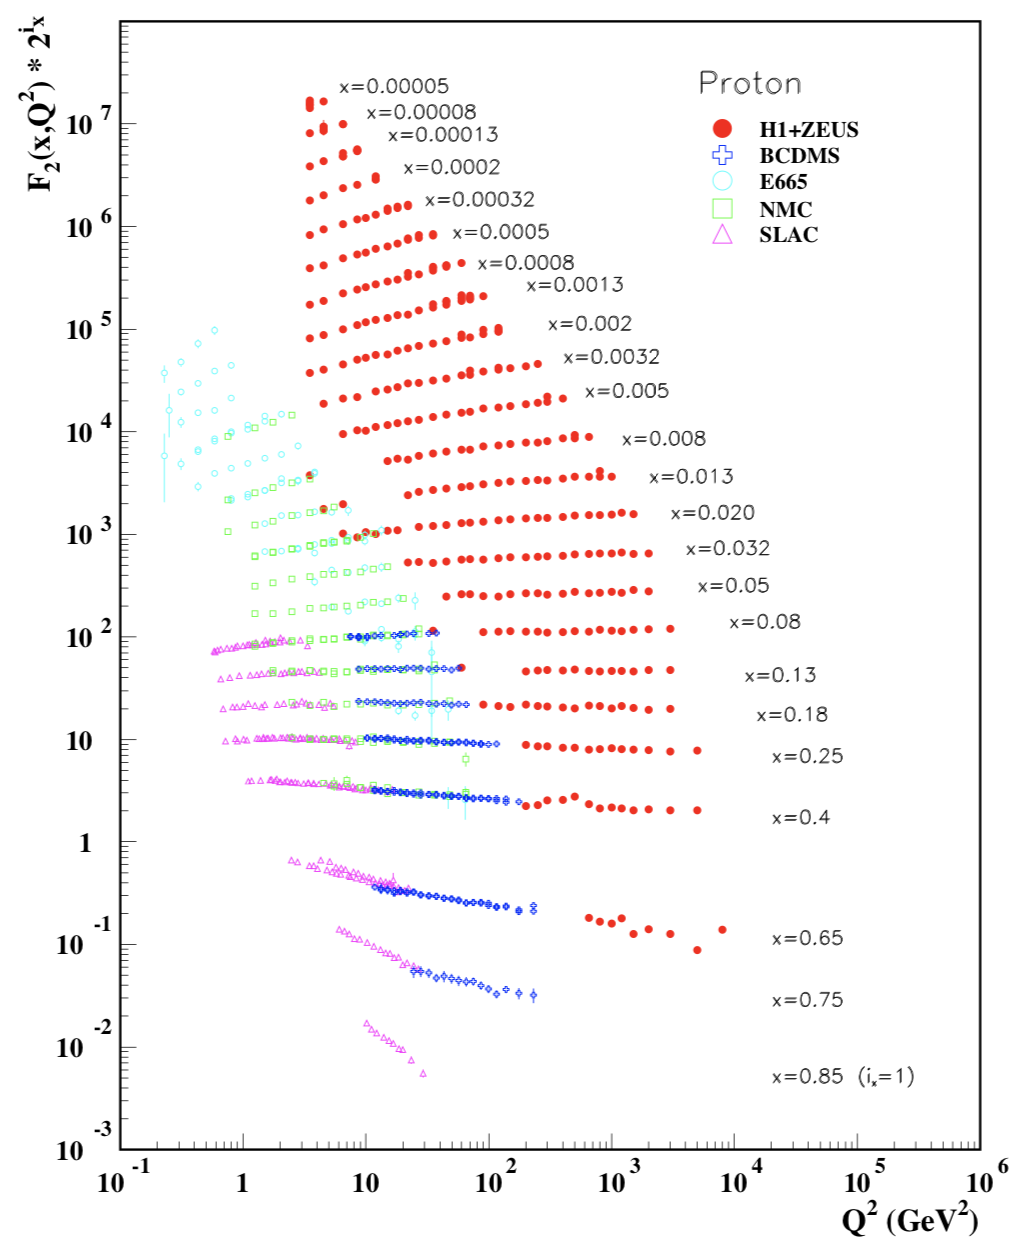
\includegraphics[scale=0.65]{./gfx/F2.png}
	\caption{The proton structure function $F^2_p$ measured in electromagnetic scattering of electrons and positrons on protons in the kinematic domain of the HERA data (collider experiments H$1$ and ZEUS for $Q^2 \geq 2$ GeV$^2$), and for electrons (SLAC) and muons (BCDMS, E$665$, NMC) on a fixed target. Figure taken from \cite{PDG}.}
	\label{pic:F2}
\end{figure}

\subsection{QCD-improved QPM}

The $Q^2$ dependence mentionned in previous subsection can be estimated by introducing quark interactions in the framework of QCD \cite{DISmeas,PICH}. Quantum ChromoDynamics is a non-abelian gauge theory based on a symmetry group SU($3$), which describes the interaction of quarks and gluons. The charge of this theory is called colour and the force carriers are the gluons, which are also coloured particles. The internal nucleon dynamic is due to the gluon emission and absorption and quark-antiquark pair creation from gluons. This creates a cloud of gluons and virtual $q\bar{q}$ pairs known as sea quarks.

The QCD coupling constant $\alpha_s$ depends on the scale of the interaction. At low energies quarks or gluons are always forming colorless particles, which are named hadrons : this is called confinement. At high energies quarks or gluons are free particles : this is asymptotic freedom.

Depending on the energy regime, a process can be labeled as a hard ($\alpha_s \sim 0$) or soft process ($\alpha_s large$). Hard processes can be described within the perturbative QCD (pQCD) framework, while soft processes can only be parametrized from experimental data. As in DIS the scale variable is often chosen as $Q^2$, the DIS cross-section is factorized \cite{CollinsSoper} in terms of soft and hard processes for $Q^2 > 1$ GeV$^2$, where $\alpha_s$ is small enough : the hard process is described by the lepton-quark cross-section $\sigma_q$ convoluted with the soft process parametrized by the PDFs. These two regimes differ by the factorisation scale $\Lambda$ that is mostly chosen as $Q^2$.

The resolution of the virtual photon probe is proportional to $1/Q^2$ (see Fig.~\ref{pic:Q2res} at fixed $x$). At $Q^2 \sim 0$, the virtual photon sees the nucleon as a point-like particle. As $Q^2$ increases, the virtual photon starts to resolve the nucleons constituents. At large $Q^2$ the virtual photon is able to resolve point-like quarks. The first QCD correction to the QPM concerns the gluon emission by the initial and the final quark.

\begin{figure}[!h]
  \centering
	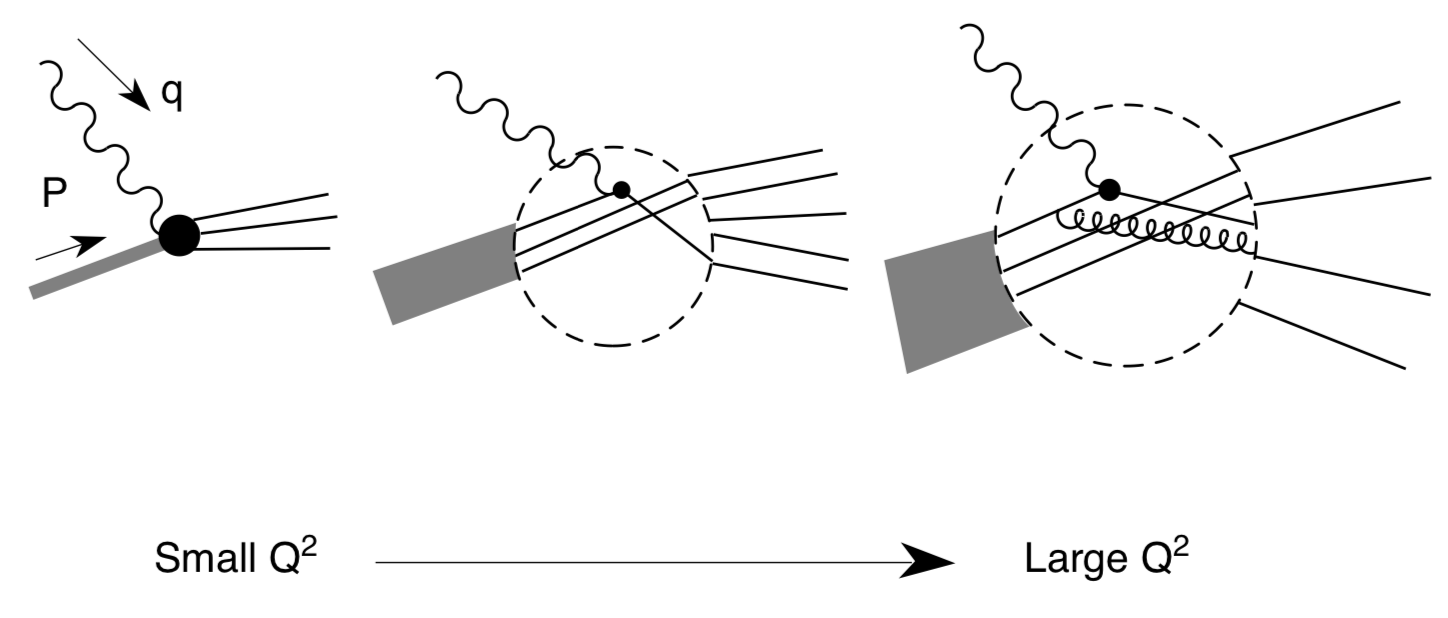
\includegraphics[scale=0.6]{./gfx/Q2res.png}
	\caption{Resolution of the photon probe versus $Q^2$. Figure taken from \cite{PICH}.}
	\label{pic:Q2res}
\end{figure}

The $Q^2$ dependence can be calculated using the Dokshiter-Gribov-Lipatov-Altarelli-Parisi (DGLAP) equations \cite{Dokshitser, GL1, GL2, AP} :
%
\begin{equation}
  \frac{dq_i(x,Q^2)}{dlnQ^2} = \frac{\alpha_s(Q^2)}{2\pi}\sum\limits_{j}\int_{x}^{1}P_{ij}(x/\xi,\alpha_s(Q^2))q_i(\xi,Q^2).
\end{equation}
%
Here, the splitting functions $P_{ij}(x/\xi)$ \cite{Joosten} are the probability that a quark or gluon of type $j$ and momentum fraction $\xi$ is the parent of $i$ with momentum fraction $x$. A similar equation holds for the gluon distribution. If the PDFs are known at a given scale $Q_0^2$, they can be evolved to any given $Q^2$ using these equations.

%----------------------------------------------------------------------------------------

\section{Determination of Parton Distribution Functions}

The PDFs are non-perturbative quantities and thus cannot be calculated from a theoretical framework. A global fit to world data is the only way to quantify them. It is possible to fit measurement coming from different processes because PDFs are universal quantities, i.e. they are process independent. The world data consists mostly of lepton-nucleon DIS but collider experiments ($pp$ or $p\bar{p}$) or neutrino scattering can be used for special contributions, e.g. for gluons or strange quarks. As experiments cover different kinematic ranges, this allows one to determine the PDFs in a large ($x$,$Q^2$) space.

For the fit to be performed, a functional form has to be provided at an initial scale $Q^2_0$. Often the form $xq_i(x,Q^2_0) = x^{\alpha}(1-x)^{\beta}$, where $q_i$ are partons, is used with additional terms refining the fit, reaching a number of free parameters from $10$ to $25$. The DGLAP equations are then used to evolve the PDFs to a given $Q^2$. An example of a fit done by the MMHT group \cite{MMHT} at Next to Leading Order (NLO) for different $Q^2$ values is shown in Fig.~\ref{fig:MMHT}.

\begin{figure}[htb!]
\centerline{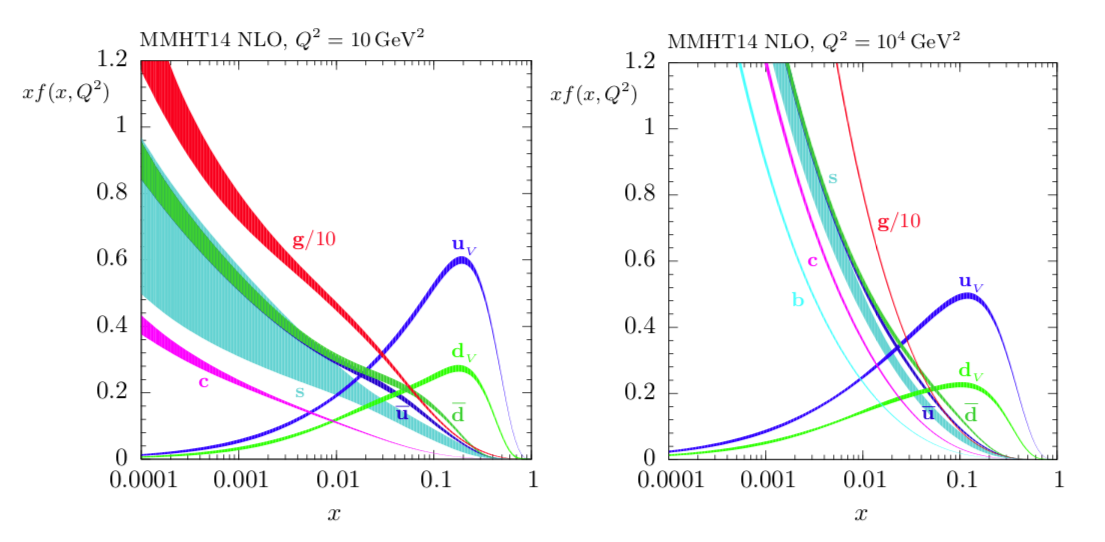
\epsfig{file=gfx/MMHT.png,width=14cm}}
\caption{Unpolarized PDFs at Next to Leading Order (NLO) from MMHT group at $Q^2$ = $10$ GeV$^2$ (left) and $Q^2$ = $10^4$ GeV$^2$ (right) with associated 68\% confidence-level uncertainty bands. Figure taken from \cite{MMHT}.}\label{fig:MMHT}
\end{figure}

%----------------------------------------------------------------------------------------

\section{Semi-Inclusive Deep Inelastic Scattering}

SIDIS is the semi-inclusive measurement of DIS. In the final state, at least one hadron and the scattered lepton are detected ($l+N \rightarrow l'+h+X$) and a new invariant variable $z$ is introduced, which corresponds to the energy fraction of the virtual photon held by the hadron $h$ :
%
\begin{equation}
  z = \frac{\textbf{P}\cdot\textbf{p}_h}{\textbf{P}\cdot\textbf{q}} \stackrel{lab}{=} \frac{E_h}{\nu}.
  \label{eq:SIDIS}
\end{equation}
%
The semi-inclusive cross section reads \cite{SIDISXS}:
%
\begin{equation}
  \frac{d\sigma}{dxdydz} = \frac{8\pi\alpha^2ME}{Q^4}\left[xy^2H_1(x,Q^2,z)+(1-y)H_2(x,Q^2,z)\right],
  \label{eq:SIDISXS}
\end{equation}
%
where $H_1$ and $H_2$ are structure functions related to $F_1$ and $F_2$ \cite{BERGER,SIDISXS} :
%
\begin{equation}
  \sum\limits_{h}\int_{0}^{1} H_i(x,Q^2,z)dz = F_i(x,Q^2)\quad,\quad i \in  \llbracket1,2\rrbracket.
\end{equation}
%
Additional variables used to describe the hadron kinematics are given in Table.~\ref{tab:SIDIS}.

\begin{table}[h!]
  \caption{SIDIS kinematic variables.}
  \label{tab:SIDIS}
  \begin{tabularx}{\textwidth}{r|lX}
    \hline
    \hline
    Variable & Description \\
    \hline
    \hline
    $\textbf{p}=(E_h,\vec{p}_h)$ & Hadron $4$-momentum vector \\
    $p_{h\|}$ & Component of $\vec{p}_h$ along $\vec{q}$ \\
    $p_{h\bot}$ & Transverse component of $\vec{p}_h$ with respect to $\vec{q}$ \\
    $\theta_h$ & Angle between $\vec{q}$ and $\vec{p}_h$ \\
    $\Phi_h$ & Angle between the scattering plane and the hadron production plane \\
    $z=\frac{E_h}{\nu}$ & Energy fraction of the virtual photon transferred to the hadron $h$ \\
    $\eta=\frac{1}{2}\text{ln}\left(\frac{|\mathbf{p}|+p_L}{|\mathbf{p}|-p_L} \right)$ & Pseudorapidity \\
    \hline
    \hline
  \end{tabularx}
\end{table}

\subsection{SIDIS in QPM}

The factorization Ansatz is also valid for SIDIS measurement thus the hadron production can be described as a convolution of three independent processes : the soft part $q(x)$ that are the PDFs, the hard process $\sigma_q$ describing the absorption of the virtual photon $\gamma^*$ by the quark $q$ and the soft part $D_q^h(z)$ characterize the fragmentation of the quark $q$ into a hadron $h$.

\begin{figure}[!h]
  \centering
	% 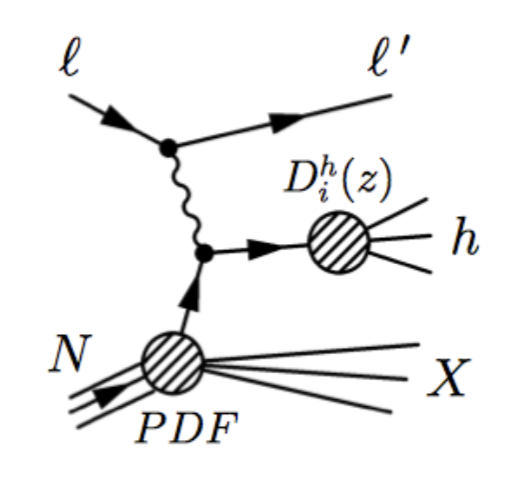
\includegraphics[scale=0.6]{./gfx/SIDIS.png}
  \begin{tikzpicture} \begin{feynman}
  \vertex (i1) {\(l\)};
  \vertex[right=2cm of i1] (a);
  \vertex[above right=2cm of a] (i2) {\(l'\)};
  \vertex[blob,below=2cm of a] (b) {\(\sigma_q\)};
  \vertex[blob,below left=2cm of b] (c) {\(q(x)\)};
  \vertex[below left=2cm of c] (f12) {\(N\)};
  \vertex[right=2cm of c] (f22);
  \vertex[below=0.3cm of f22] (f23);
  \vertex[above=0.3cm of f22] (f21);
  \vertex[blob, right=of b] (d) {\(D^h_q(z)\)};
  \vertex[above right=of d] (d1) {\(h^{\pm}\)};
  \vertex[right=of d] (d2) {\(\pi^{\pm}\)};
  \vertex[below right=of d] (d3) {\(K^{\pm}\)};

  \diagram* { (i1) -- [fermion] (a) -- [fermion] (i2),
  (a) -- [photon, edge label=\(\gamma^*\)] (b) [blob],
  (c) [blob] -- [fermion] (b) [blob],
  (b) [blob] -- [fermion] (d) [blob],
  (f12) -- [double distance=7pt] (c) [blob] -- [plain] (f22),
  (f12) -- [fermion] (c) [blob],
  (c) [blob] -- [plain] (f21),
  (c) [blob] -- [plain] (f23),
  (d) [blob] -- [plain] (d1),
  (d) [blob] -- [plain] (d2),
  (d) [blob] -- [plain] (d3),
  };
  \draw [decoration={brace}, decorate] (f21.north east) -- (f23.south east) node [pos=0.5, right] {\(X\)};
  \end{feynman} \end{tikzpicture}
	\caption{Factorization in SIDIS.}
	\label{pic:SIDIS}
\end{figure}

The structure functions $H_i(x,Q^2,z)$ contain the information on what happens to the struck quark after the interaction with the virtual photon. The fragmentation function (FF) $D_q^h(z,Q^2)$ is defined as the probability for a quark of flavour $q$ to fragment into a hadron $h$ with a fraction of energy $z$. The expression of the spin averaged SIDIS cross section can be expressed within QPM at LO in terms of PDFs and FFs \cite{BERGER,Panknin} :
%
\begin{equation}
  \frac{d^3 \sigma}{dxdydz} \stackrel{LO}{=} \frac{8\pi\alpha^2ME}{Q^2}\left[\frac{1}{2}y^2+\left(1-y-\frac{y^2 \gamma^2}{4}\right)\right]x\sum\limits_qe^2_qq(x)D_q^h(z).
  \label{eq:unpolSIDIS}
\end{equation}

%----------------------------------------------------------------------------------------

\section{Fragmentation Functions}\label{sec:FF}

When computing the cross-section of a given process $A+B \rightarrow h+X$, this cross-section is found to be a convolution of three different terms (Eq.~\ref{eq:facto}) : one non-perturbative term involving the PDFs (probability to obtain parton $a$ from nucleus $A$ $f_{a/A}(x_a,Q^2)$), one hard cross-section term for perturbative calculation ($d\sigma_{a,b \rightarrow c}(x_a,x_b,Q^2)$) and a last non-perturbative term involving the FFs (probability to obtain hadron $h$ from parton $c$ $D^h_c(x_c,Q^2)$).
%
\begin{equation}
  d\sigma_{A+B \rightarrow h+X} = \sum_{a,b,c} \left[ f_{a/A}(x_a,Q^2) f_{b/B}(x_b,Q^2) \right] \otimes \left[ d\sigma_{a,b \rightarrow c}(x_a,x_b,Q^2) \right] \otimes \left[ D^h_c(x_c,Q^2) \right]
  \label{eq:facto}
\end{equation}
%
Fig.~\ref{pic:SIDIS} illustrates this factorization in SIDIS. The extraction of FFs can also be done from electron-positron annihilation and hadron-hadron collisions measurements. The universality of FFs has been experimentally tested by Kniehl, Kramer and Pötter \cite{Universality}. Different ideas have been developed to model how quarks confine together to make a hadron.

\subsection{Lund String Fragmentation Model}

In the Lund String Model \cite{LUND}, the hadron production is explained by the creation of quark-antiquark pairs $q\bar{q}$. The strong interaction between partons is represented by a string. The energy inside the string is linear function of the distance between two stringed partons. At some point the energy is large enough to create a new $q\bar{q}$ pair and the string breaks. All unpaired remnants have new strings and the process repeats until there are only hadrons. The hadronization scheme in the Lund model in the center of mass frame is illustrated in Fig.~\ref{pic:Lund} (a). The virtual photon is absorbed e.g. by a $u$ quark and in consequence the $u$ quark is ejected from the nucleon. A new $q\bar{q}$ pair is created by the string breaking e.g. $d\bar{d}$. The remaining $u$ quark binds with the $\bar{d}$ quark to form a $\pi^+$ with a given $z$ as shown in Fig.~\ref{pic:Lund} (b). The remaining system repeats fragmentation process until the energy is smaller than the available energy $\nu$. In addition baryon creation by di-$q\bar{q}$ pair formation is introduced.

\begin{figure}[!h]
  \centering
	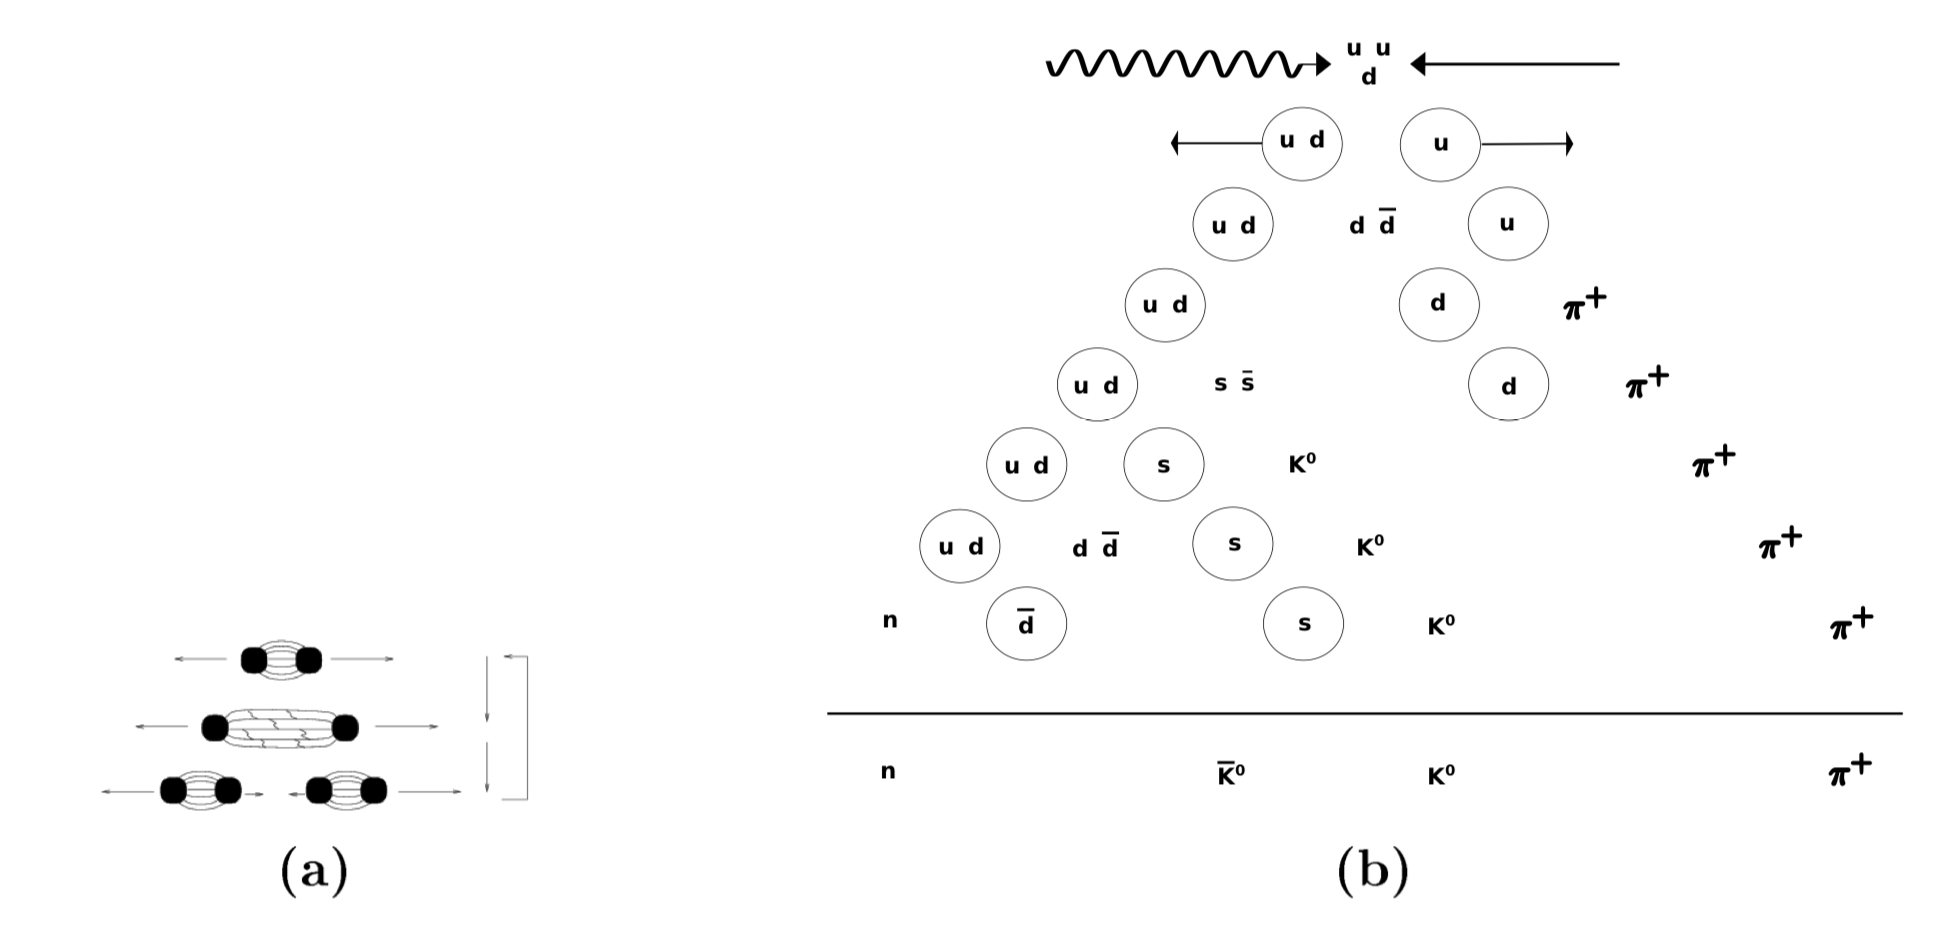
\includegraphics[scale=0.45]{./gfx/Lund.png}
	\caption{The fragmentation process in the Lund model. In (b), the produced $K^0$, $\overline{K^0}$, $\pi^+$ or $n$ could also be an excited state. Figure taken from \cite{Panknin}.}
	\label{pic:Lund}
\end{figure}

\subsection{Quark Fragmentation Regions}

Up to this point only the fragmentation of the struck quark was considered. The spectator quarks, which are not involved in the scattering process, have also to hadronize. This phenomenon is happening in two distinct $p_h$ regions : the target fragmentation region, where the final hadron $h$ has a small momentum in the rest frame of the target, and the current fragmentation region, where the product $\textbf{P}\cdot\textbf{p}_h$ grows with $Q^2$. At low energies there is a large overlap of these regions, while at high energies they start to separate. This hadron production can contaminate the SIDIS measurement of current fragmentation. To deal with this issue, Berger \cite{BERGER} came with a criterion based on the pseudorapidity of the final state $\eta$, which is the measurement of the longitudinal momentum. The sign of $\eta$ is linked to the different regions : if $\eta$ $>$ $0$ the hadron moves towards the direction of the virtual photon and is a current hadron, else is $\eta$ $<$ $0$ the hadron is a target remnant (Fig.~\ref{pic:Berger}). Defining $p(k)$ to be the probability that $k$ hadrons of some specific type decay from one cluster, one finds that the \textit{fully inclusive} correlation function has the form :
%
\begin{equation}
  C(y_1,y_2) = \frac{\langle k(k-1) \rangle}{\langle k \rangle} \left(\frac{1}{\sigma}\frac{d\sigma}{dy}\right)_{y\sim 0} G(y_1-y_2),
\end{equation}
%
when $y_1$ and $y_2$ are in the central region and the averages are :
%
\begin{equation}
  \begin{split}
    \langle k \rangle = \sum kp(k) \\
    \langle k-1 \rangle = \sum k(k-1)p(k).
  \end{split}
\end{equation}
%
The Gaussian function :
%
\begin{equation}
  G(y_1-y_2) = \frac{1}{2\delta \sqrt{\pi}}exp\left[-\frac{\left(y_1-y_2\right)}{4\delta^2}\right],
\end{equation}
%
has an effective \textit{correlation length} of $2\delta$. As the typical hadronic correlation length in pseudorapidity is $\delta \sim 2$, a separation criterion, the Berger criterion, is that $\Delta\eta = \eta_{max}-\eta_{min} \geq 2\delta$ or in terms of DIS kinematics variables $W \gtrsim 7.4$ GeV. It is important to select the kinematic region so that selected hadrons are dominated by the struck quark fragmentation.

\begin{figure}[!h]
  \centering
	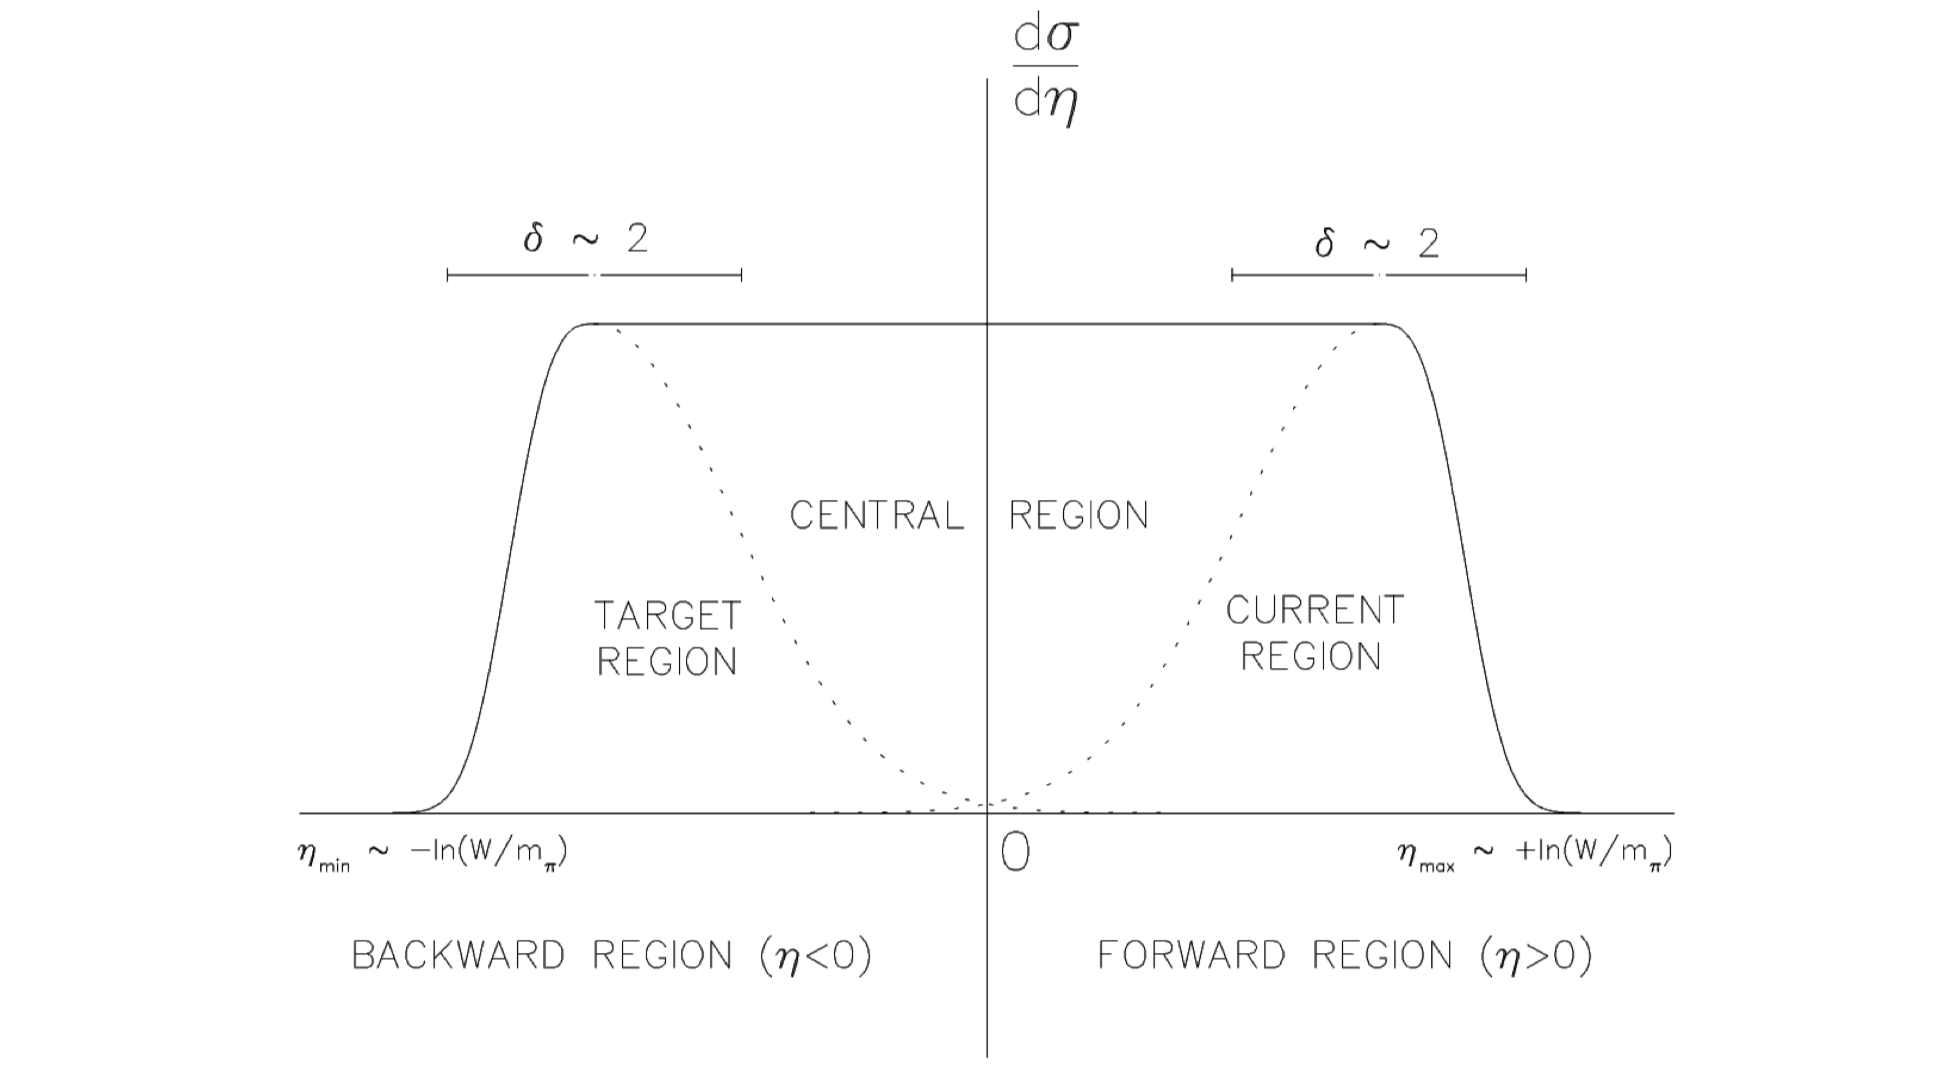
\includegraphics[scale=0.5]{./gfx/Berger.png}
	\caption{Hadronic pseudorapidity ($\eta$) distribution at very high energies. Figure taken from \cite{Niczy}.}
	\label{pic:Berger}
\end{figure}

\subsection{Scaling and $Q^2$ evolution}

For the FFs extracted from $e^+e^-$ annihilation displayed in Fig.~\ref{pic:FFscale}, the scaling is present for a wide $x = 2p_h/\sqrt{s}$ range (Fig.~\ref{pic:FFscale} (a)). At low x ($x$ $<$ $0.1$) the FFs increases with the total center-of-mass energy $\sqrt{s}$ (Fig.~\ref{pic:FFscale} (b)), while at large $x$, the FFs are shifted towards lower values for large $Q^2$ (similar behaviour as PDFs). Here $\sqrt{s}$ has the same role has $Q^2$. Scaling violation is observed \cite{PDG}.

\begin{figure}[!h]
  \centering
	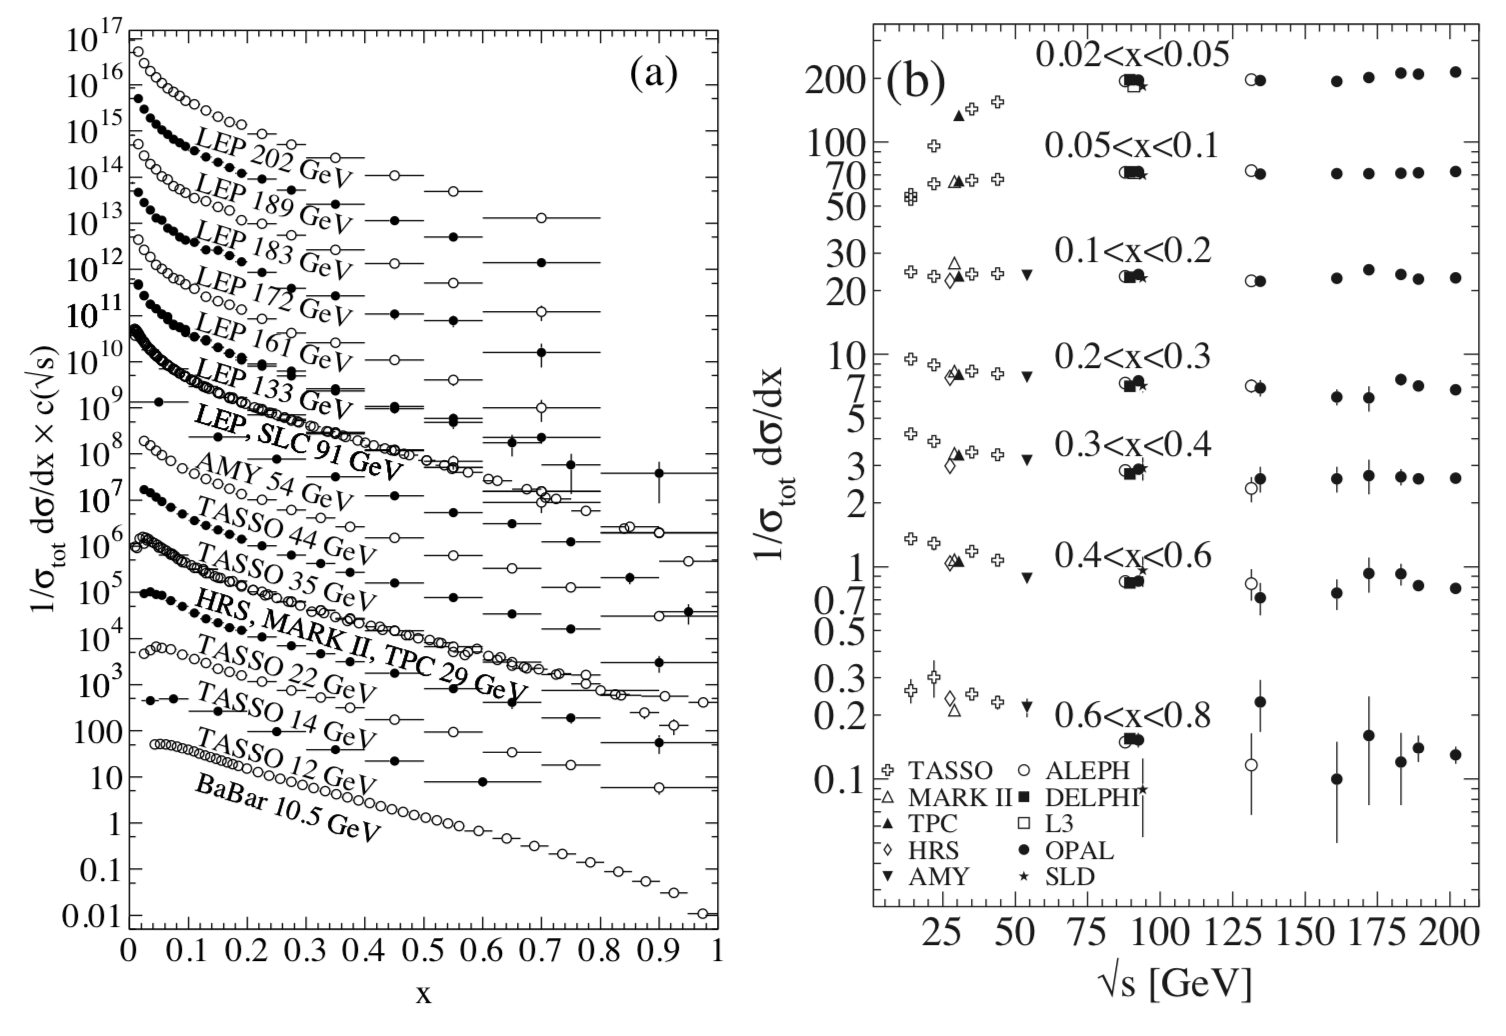
\includegraphics[scale=0.6]{./gfx/FFscale.png}
	\caption{The $e^+ e^-$ fragmentation function for all charged particles for different center of mass energy $\sqrt{s}$ versus $x$ (a) and for various range of $x$ versus $\sqrt{s}$ (b). Figures taken from \cite{PDG}.}
	\label{pic:FFscale}
\end{figure}

The evolution of the fragmentation functions is also described by DGLAP equations \cite{Dokshitser, GL1, GL2, AP} :
%
\begin{equation}
  \frac{dD_q^h(z,Q^2)}{dlnQ^2} = \frac{\alpha_s(Q^2)}{2\pi}\sum\limits_j\int_{x}^{1}P_{qj}\left(z/\xi,\alpha_s(Q^2)\right)D_q^h(\xi,Q^2)\frac{d\xi}{\xi}.
\end{equation}
%
In Fig.~\ref{pic:QuarkFrag} the process contributing to the $Q^2$-evolution is illustrated~: the fragmentation of a quark $q_i$ through its own hadronization after emmiting a gluon $G$ ($P_{qq}D_{q_i}^h$), through the hadronization of a gluon $G$ ($P_{Gq}D_{G}^h$), the fragmentation of a gluon splitting into a quark-antiquark pair and following hadronization of the quark in hadron ($P_{qG}D_{q_i}^h$) and eventually the gluon fragmentation via the three-gluon self-interaction ($P_{GG}D_{G}^h$).

\begin{figure}[!h]
  \centering
	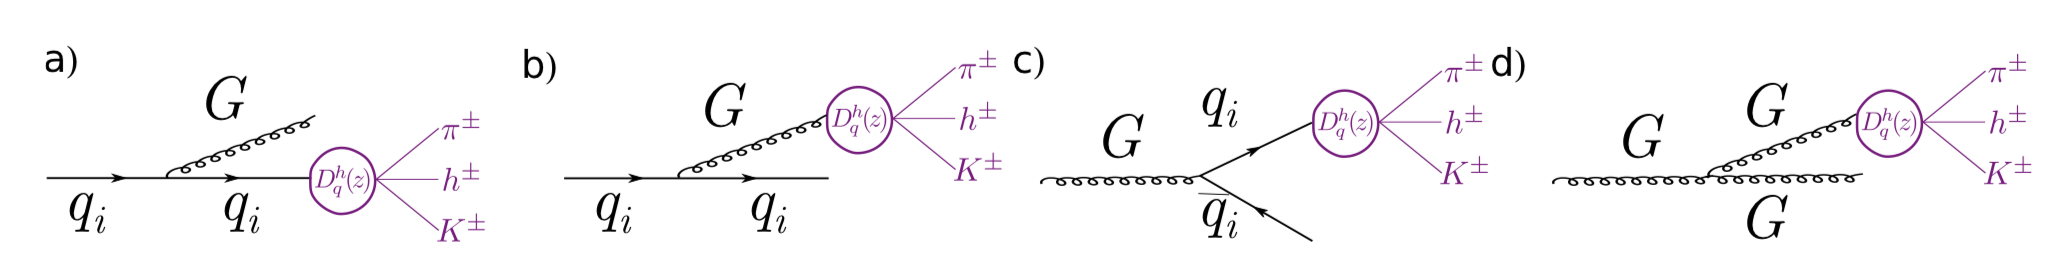
\includegraphics[scale=0.45]{./gfx/QuarkFrag.png}
	\caption{The fragmentation of the quark $q_i$ decaying into a hadron $h$ while emitting a gluon $G$ ($P_{qq}D^h_{q_{i}}$) (a), the fragmentation of the quark $q_i$ through a gluon $G$ ($P_{Gq}D^h_{G}$) (b), the fragmentation of the gluon $G$ via the creation of a $q_i \bar{q_i}$ pair and the decay of $q_i$ ($P_{qG}D^h_{q_{i}}$) (c) and the fragmentation of the gluon $G$ via a three gluon vertex ($P_{GG}D^h_{G}$) (d). Figure taken from \cite{Uematsu}.}
	\label{pic:QuarkFrag}
\end{figure}

\subsection{Fragmentation Function Symmetries}

One FF $D^h_q(z,Q^2)$ is introduced for each flavour $q$ and each hadron species $h$. Considering only the light quarks ($u$,$\bar{u}$,$d$,$\bar{d}$,$s$ and $\bar{s}$), in case the mass threshold for heavy quarks is higher than the covered kinematic domain, implies that for charged hadrons one has to measure twelve different fragmentation functions for positive and negative hadrons. Nevertheless, within the QCD-improved QPM, symmetries as isospin or charge-conjugation can be used to reduce the number of independent fragmentation functions.

The FFs can be split into two main categories. If a quark fragments into a hadron h and the quark is a valence quark of $h$, the FF is said to be favoured ($D^h_{fav}$). If it is a sea quark of $h$, the FF is unfavoured ($D^h_{unf}$).

For pions charge-conjugation symmetry reduces the number of independent fragmentation functions to six. The application of the isospin (viz. $D^{\pi^+}_u = D^{\pi^+}_{\bar{d}}$ for $\pi^+$) and SU($3$) symmetries lowers this number further to two :
%
\begin{equation}\label{eq:FFPion}
  \begin{split}
    D^h_{fav} : D^{\pi^+}_u = D^{\pi^-}_{\bar{u}} = D^{\pi^-}_d = D^{\pi^+}_{\bar{d}}, \\
    D^h_{unf} : D^{\pi^-}_u = D^{\pi^+}_{\bar{u}} = D^{\pi^+}_d = D^{\pi^-}_{\bar{d}} \stackrel{SU(3)\,sym.}{=} D^{\pi^{\pm}}_s = D^{\pi^{\mp}}_{\bar{s}}.
  \end{split}
\end{equation}

For kaons charge-conjugation symmetry reduces the number of independent fragmentation functions to six. The application of the isospin (viz. $D^{\pi^+}_u = D^{\pi^+}_{\bar{d}}$ for $\pi^+$) and SU($3$) symmetries lower the number to three independent FFs : the favoured, grouping the kaons valence quarks $u$ and $\bar{u}$ FFs, the strange, grouping the kaons valence quarks $s$ and $\bar{s}$ FFs and the unfavoured, grouping the kaons sea quark FFs :
%
\begin{equation}\label{eq:FFKaon}
  \begin{split}
    D^h_{fav} : D^{K^+}_u = D^{K^-}_{\bar{u}} \\
    D^h_{str} : D^{K^+}_{\bar{s}} = D^{K^-}_{s} \\
    D^h_{unf} : D^{K^+}_{\bar{u}} = D^{K^-}_{u} = D^{K^+}_s = D^{K^-}_{\bar{s}} = D^{K^{\pm}}_{d} = D^{K^{\mp}}_{\bar{d}}
  \end{split}
\end{equation}

%----------------------------------------------------------------------------------------

\section{State of the art of the fragmentation functions}

\subsection{Measurements}

The production of hadrons from the the struck quark cannot be computed as final state hadron masses are of order or smaller than $\Lambda_{QCD}$. In order to extract FFs reliably from the $Q^2$ dependence of the measured hadron production, a large kinematic range is needed. Thus data taken at different energies are used. Three different processes are so far used to extract quark fragmentation functions : electron-positron annihilation (SIA), lepton-nucleon (SIDIS) and hadron-hadron collisions ($pp$ or $p\bar{p}$). A summary of the aspects of the different processes can be found in Table.~\ref{tab:FFProcesses}. The SIA data (LEP \cite{LEP1,LEP2,LEP3}, SLAC \cite{SLAC1}, BaBar \cite{BABAR} and BELLE \cite{BELLE}) provide the cleanest access to the FFs, since the cross-section of the process does not involve PDFs and are well calculated up to NNLO. But due to the dependence of the cross-section on $e^2_q$, $D^h_q$ and $D^h_{\bar{q}}$ cannot be separated and there is a limited access to gluon FF $D^h_g$. The data from hadron-hadron collisions (UA5 \cite{UA5}, UA1 \cite{UA1}, ALICE \cite{ALICE}, CMS \cite{CMS1,CMS2}, ATLAS \cite{ATLAS}, RHIC \cite{RHIC1,RHIC2,RHIC3}) give access to $D^h_q$, $D^h_{\bar{q}}$ and $D^h_g$, but allow no direct access to $z$.

Data from SIDIS can be compared to data from previously presented processes for the current fragmentation region (see Section~\ref{sec:FF}). SIDIS data have the advantage that factorization has been proven to all orders of $\alpha_s$. In addition they cover a wide range in $Q^2$ in a single measurement compared to SIA. The experiments providing inputs for the SIDIS process are EMC \cite{EMC} and COMPASS \cite{COMPASS2006Pi,COMPASS2006K} using muon beam and E$00$-$108$ \cite{E00108} and HERMES \cite{HERMESMult} using electron beam. All experiments measured with proton and deuteron targets.

\begin{table}[!h]
  \caption{Fragmentation functions access for different processes.}
  \label{tab:FFProcesses}
  \centering
  \begin{tabular}{cccc}
    \hline
    \hline
    & $e^+ e^- annihilation$ & $pp$/$p\bar{p}$ collision & DIS \\
    \hline
     &   \resizebox{3cm}{3.5cm}{\begin{tikzpicture} \begin{feynman}
     \vertex (i1) {\(e^{-}\)};
     \vertex[right=2cm of i1] (a);
     \vertex[above right=2cm of a] (i2) {\(e^{+}\)};
     \vertex[blob,below=2cm of a] (b) {\(\widehat{\sigma_q}\)};
     \vertex[below left=2cm of b] (f12);
     \vertex[below=0.3cm of f12] (f13);
     \vertex[above=0.3cm of f12] (f11);
     \vertex[blob,below right=2cm of b] (d) {\(D^h_q(z)\)};
     \vertex[above right=of d] (d1) {\(h^{\pm}\)};
     \vertex[right=of d] (d2) {\(\pi^{\pm}\)};
     \vertex[below right=of d] (d3) {\(K^{\pm}\)};

     \diagram* { (i1) -- [fermion] (a) -- [anti fermion] (i2),
     (a) -- [photon, edge label=\(\gamma^{*}/Z^{0}\)] (b) [blob],
     (f12) -- [plain] (b) [blob] -- [fermion] (d) [blob],
     (f13) -- [plain] (b) [blob],
     (f11) -- [plain] (b) [blob],
     (d) [blob] -- [plain] (d1),
     (d) [blob] -- [plain] (d2),
     (d) [blob] -- [plain] (d3),
     };
     \draw [decoration={brace}, decorate] (f13.south west) -- (f11.north west) node [pos=0.5, left] {\(X\)};
   \end{feynman} \end{tikzpicture}}
      & \resizebox{3.5cm}{3cm}{\begin{tikzpicture} \begin{feynman}
    \vertex (i1) {\(p\)};
    \vertex[blob,right=2cm of i1] (a) {\(q(x)\)};
    \vertex[below=6cm of i1] (i2) {\(p/\bar{p}\)};
    \vertex[blob,right=2cm of i2] (b) {\(q(x)\)};
    \vertex[blob,below right=4cm of a] (c) {\(\widehat{\sigma}_q\)};
    \vertex[above right=of c] (f1);
    \vertex[blob, below right=of c] (d) {\(D^h_q(z)\)};
    \vertex[above right=of d] (d1) {\(h^{\pm}\)};
    \vertex[right=of d] (d2) {\(\pi^{\pm}\)};
    \vertex[below right=of d] (d3) {\(K^{\pm}\)};

    \diagram* { (i1) -- [double distance=7pt] (a) [blob], (i1) -- [fermion] (a) [blob],
    (i2) -- [double distance=7pt] (b) [blob], (i2) -- [fermion] (b) [blob],
    (a) -- [fermion] (c) [blob], (b) -- [fermion] (c) [blob], (c) [blob] -- [fermion] (f1), (c) [blob] -- [fermion, edge label=\(q\)] (d) [blob],
    (d) [blob] -- [plain] (d1),
    (d) [blob] -- [plain] (d2),
    (d) [blob] -- [plain] (d3),
    };
    \end{feynman} \end{tikzpicture}}
      & \resizebox{3cm}{3.5cm}{\begin{tikzpicture} \begin{feynman}
      \vertex (i1) {\(l\)};
      \vertex[right=2cm of i1] (a);
      \vertex[above right=2cm of a] (i2) {\(l'\)};
      \vertex[blob,below=2cm of a] (b) {\(\widehat{\sigma}_q\)};
      \vertex[blob,below left=2cm of b] (c) {\(q(x)\)};
      \vertex[below left=2cm of c] (f12) {\(N\)};
      \vertex[right=2cm of c] (f22);
      \vertex[below=0.3cm of f22] (f23);
      \vertex[above=0.3cm of f22] (f21);
      \vertex[blob, right=of b] (d) {\(D^h_q(z)\)};
      \vertex[above right=of d] (d1) {\(h^{\pm}\)};
      \vertex[right=of d] (d2) {\(\pi^{\pm}\)};
      \vertex[below right=of d] (d3) {\(K^{\pm}\)};

      \diagram* { (i1) -- [fermion] (a) -- [fermion] (i2),
      (a) -- [photon, edge label=\(\gamma^*\)] (b) [blob],
      (c) [blob] -- [fermion] (b) [blob],
      (b) [blob] -- [fermion] (d) [blob],
      (f12) -- [double distance=7pt] (c) [blob] -- [plain] (f22),
      (f12) -- [fermion] (c) [blob],
      (c) [blob] -- [plain] (f21),
      (c) [blob] -- [plain] (f23),
      (d) [blob] -- [plain] (d1),
      (d) [blob] -- [plain] (d2),
      (d) [blob] -- [plain] (d3),
      };
      \draw [decoration={brace}, decorate] (f21.north east) -- (f23.south east) node [pos=0.5, right] {\(X\)};
    \end{feynman} \end{tikzpicture}}\\
    Dependence & $\widehat{\sigma} \otimes FF$ & $\widehat{\sigma} \otimes PDF \otimes PDF \otimes FF$ & $\widehat{\sigma} \otimes PDF \otimes FF$ \\
    Separate $D^h_{q}$ / $D^h_{\bar{q}}$ & \ding{55} & \ding{51} & \ding{51} \\
    Access parton kinematics & \ding{51} & \ding{55} & \ding{51} \\
    Theoretical calculation & LO, NLO, NNLO & LO, NLO & LO, NLO \\
    \hline
  \end{tabular}
\end{table}

\subsection{Accessing the fragmentation functions in SIDIS}

Hadron multiplicities are defined as the cross-section ratio :
%
\begin{equation}
  M^h(x,Q^2,z) = \frac{d\sigma^{lN \rightarrow l'hX}}{d\sigma^{lN \rightarrow l'X}dz} = \frac{d\sigma^h(x,Q^2,z)/dxdQ^2dz}{d\sigma^{DIS}(x,Q^2)/dxdQ^2},
\end{equation}
%
equivalent to the number of hadrons produced per DIS events allowing to access FFs by measuring hadron multiplicities.

Using the expressions of the DIS and SIDIS cross-sections (Eqs.~\ref{eq:unpolDIS} and \ref{eq:unpolSIDIS}) one obtains in the QPM :
%
\begin{equation}\label{eq:MFFPDF}
  M^h(x,Q^2,z) = \frac{\sum_q e^2_q q(x,Q^2) \otimes D^h_q(z,Q^2)}{\sum_q e^2_q q(x,Q^2)} \stackrel{LO}{=} \frac{\sum_q e^2_q q(x,Q^2) D^h_q(z,Q^2)}{\sum_q e^2_q q(x,Q^2)}.
\end{equation}
%
As PDFs and FFs depend on different variables $x$ and $z$ one can write the convolution as a single product. By measuring $M^h(x,Q^2,z)$ for positive and negative hadrons, one can distinguish $D^h_q$ and $D^h_{\bar{q}}$. The procedure of FFs extraction from COMPASS multiplicity measurement is described in Chapter~\ref{ch:FF}.

\subsection{Global fits of multiplicity data and parametrizations of FFs}

As the FFs are universal quantities, a global QCD fit of available data on multiplicities from SIA, SIDIS and $pp$/$p\bar{p}$ collisions can be performed to give a general parametrization of the FFs. There are different parametrization available in the literature. Some parametrizations are only based on SIA data : KKP \cite{Universality}, KRE \cite{KRE} and HKNS \cite{HKNS}, when the AKK \cite{AKK} parametrization uses in addition some hadron-hadron scattering data. One only uses SIDIS data : LSS \cite{LSS}. The newest parametrizations from DSEHS \cite{DSEHS1,DSEHS2} include all three types of data and JAM \cite{JAM} parametrizations include SIA+SIDIS. Each parametrization has its own set of assumptions based on symmetries and its different parametrization of $D^h_q$. A summary of the assumptions of the different groups can be found in Table \ref{tab:FFParametrization}. Only DSEHS and JAM will be described in more details in the following as they are the latest ones (or have been updated recently).

\begin{table}[!h]
  \caption{Parametrization of FFs for pions and kaons.}
  \label{tab:FFParametrization}
  \centering
  \begin{tabular}{ccccccc}
    \hline
    \hline
    Parametrization & Year & \multicolumn{3}{c}{Data} & \multicolumn{2}{c}{\# FFs fitted} \\
    \hline
     & & SIDIS & $pp$/$p\bar{p}$ & SIA & $\pi$ & $K$ \\
    KKP \cite{Universality} & 2000 & \ding{55} & \ding{55} & \ding{51} & 5 & 5 \\
    KRE \cite{KRE} & 2001 & \ding{51} & \ding{55} & \ding{51} & 2 & 3 \\
    HKNS \cite{HKNS} & 2007 & \ding{55} & \ding{55} & \ding{51} & 2 & 2 \\
    AKK \cite{AKK} & 2008 & \ding{55} & \ding{51} & \ding{51} & 3 & 5 \\
    LSS \cite{LSS} & 2014 & \ding{51} & \ding{55} & \ding{55} & 3 & 3 \\
    DSEHS \cite{DSEHS1,DSEHS2} & 2017 & \ding{51} & \ding{51} & \ding{51} & 4 & 4 \\
    JAM \cite{JAM} & 2018 & \ding{51} & \ding{55} & \ding{51} & 3 & 3 \\
    \hline
  \end{tabular}
\end{table}

\subsubsection*{DSEHS parametrization}

DSEHS (previously DSS) was the first group, who determined individual FFs for quarks and antiquarks and the first to try to fit data coming from three different processes alltogether.
The functional form they use for $D^h_q$ is the following :
%
\begin{equation}
  D^h_i (z,Q_0) = \frac{N^h_i z^{\alpha^h_i}(1-z)^{\beta^h_i}\left[ 1+\gamma^h_i(1-z)^{\delta^h_i}\right]}{B\left[2+\alpha^h_i,1+\beta^h_i\right]+\gamma^h_i B\left[2+\alpha^h_i,1+\beta^h_i+\delta^h_i\right]},
  \label{eq:DSEHSparam}
\end{equation}
%
where $N^h_i$, $\alpha^h_i$, $\beta^h_i$, $\gamma^h_i$ and $\delta^h_i$  are the fit parameters and B is the Euler beta function. For pions the two independent favoured FFs are related by a proportionality factor $k$. Moreover, isospin symmetry is considered only for the unfavoured FF ($D^{\pi^{+}}_{\bar{u}} = D^{\pi^{+}}_{d}$) and the fragmentation of a strange quark into pion is related to the unfavoured FFs with $z$-dependent factor ($D^{\pi^{+}}_{\bar{s}} = D^{\pi^{+}}_{s}=N_s z^{\alpha_s} D^{\pi^{+}}_{\bar{u}}$). Thus four FFs are fitted for pions : $u+\bar{u}$, $d=\bar{u}$, $s+\bar{s}$ and $g$. For kaons, $D^{K^+}_{u+\bar{u}}$ and $D^{K^+}_{s+\bar{s}}$ are fitted independently to account for the fact that phenomenologically it is expected that the formation of secondary $s\bar{s}$, required to form $K^+$ from a $u$, should be suppressed. Previous fits from DSS showed that $D^{K^+}_{s+\bar{s}} > D^{K^+}_{u+\bar{u}}$, highlighting this fact. For the unfavoured FFs all distributions have the same functional form  $D^{K^+}_{\bar{u}} = D^{K^+}_{s} = D^{K^+}_{d} = D^{K^+}_{\bar{d}}$ as the data are unable to discrimate between flavours. Four FFs are fitted for kaons, as for the pions :  $u+\bar{u}$, $s+\bar{s}$ , $\bar{u}=d=\bar{d}=s$ and $g$.
The FFs for heavy quarks (c,b) are also considered above their $\overline{MS}$ mass thresholds.
The parameters are determined from a standard $\chi^2$ minimization :
%
\begin{equation}
  \chi^2 =  \sum_{i=1}^{m} \left[ \left( \frac{1-\mathscr{N}_i}{\delta\mathscr{N_i}} \right) + \sum_{j=1}^{m_i} \frac{(\mathscr{N}_i T_j - E_j)^2}{\delta E^2_j} \right],
  \label{eq:DSEHSmin}
\end{equation}
%
where $m$ is the number of datasets with $m_i$ points each, $E_j$ are the data points and $\delta E_j$ their error and $T_j$ the theoretical estimate for a given set. The normalisation factor $\mathscr{N}_i$ is defined as $\delta \chi^2 / \delta\mathscr{N}_i = 0$.

\begin{table}[!h]
  \caption{DSEHS FFs hypotheses for pions and kaons.}
  \label{tab:DSEHSParametrization}
  \centering
  \begin{tabular}{ll}
    \hline
    \hline
     & Pions \\
    \hline
    Favoured & $D^{\pi^{+}}_{u} = N_{\pi^{+}} D^{\pi^{+}}_{\bar{d}}$ = $D^{\pi^{-}}_{d} = k_{\pi^{-}} D^{\pi^{-}}_{\bar{u}}$ \\
    Unfavoured & $D^{\pi^{+}}_{\bar{u}} = D^{\pi^{+}}_{d}$ \\
    Unfavoured strange & $D^{\pi^{+}}_{\bar{s}} = D^{\pi^{+}}_{s}$ \\
     & $D^{\pi^{-}}_{\bar{d}} = D^{\pi^{-}}_{u}$ = $D^{\pi^{-}}_{\bar{s}} = D^{\pi^{-}}_{s} = k_{\pi^{-}} D^{\pi^{-}}_{u}$ \\
    Gluons & $D^{\pi^{+}}_{g} = D^{\pi^{-}}_{g}$ \\
    \hline
    \hline
     & Kaons \\
    \hline
    Favoured & $D^{K^{+}}_{u}, D^{K^{-}}_{\bar{u}}$ \\
    Unfavoured & $D^{K^{+}}_{\bar{u}} = D^{K^{+}}_{d} = D^{K^{+}}_{\bar{d}} = D^{K^{+}}_{s}$ \\
               & $D^{K^{-}}_{u} = D^{K^{-}}_{d} = D^{K^{-}}_{\bar{d}} = D^{K^{-}}_{\bar{s}}$ \\
    Strange & $D^{K^{+}}_{\bar{s}}, D^{K^{-}}_{s}$ \\
    Gluons & $D^{K^{+}}_{g}, D^{K^{-}}_{g}$ \\
  \end{tabular}
\end{table}

The favoured, unfavoured and gluon FFs from DSS at LO for $Q^2$ = 10 GeV$^2$ are shown as function of $z$ for $\pi^+$ in Fig.~\ref{pic:DSEHSPi} and $K^+$ in Fig.~\ref{pic:DSEHSK}.

\begin{figure}[!h]
  \centering
	\includegraphics[scale=0.47]{./gfx/DSEHSPi.png}
	\caption{Individual FFs for positively charged pions $zD^{\pi^+}(z,Q^2)$ at $Q^2$ = $10$ GeV$^2$ (solid lines) along with uncertainty estimates at $68$\% and $90$\% C.L. indicated by the inner and outer shaded bands, respectively. The panels on the right-hand-side show the corresponding relative uncertainties. Also shown is a comparison to previous DSS$07$ global analysis \cite{DSS07} (dashed lines). Figure taken from \cite{DSEHS1}.}
	\label{pic:DSEHSPi}
\end{figure}

\begin{figure}[!h]
  \centering
	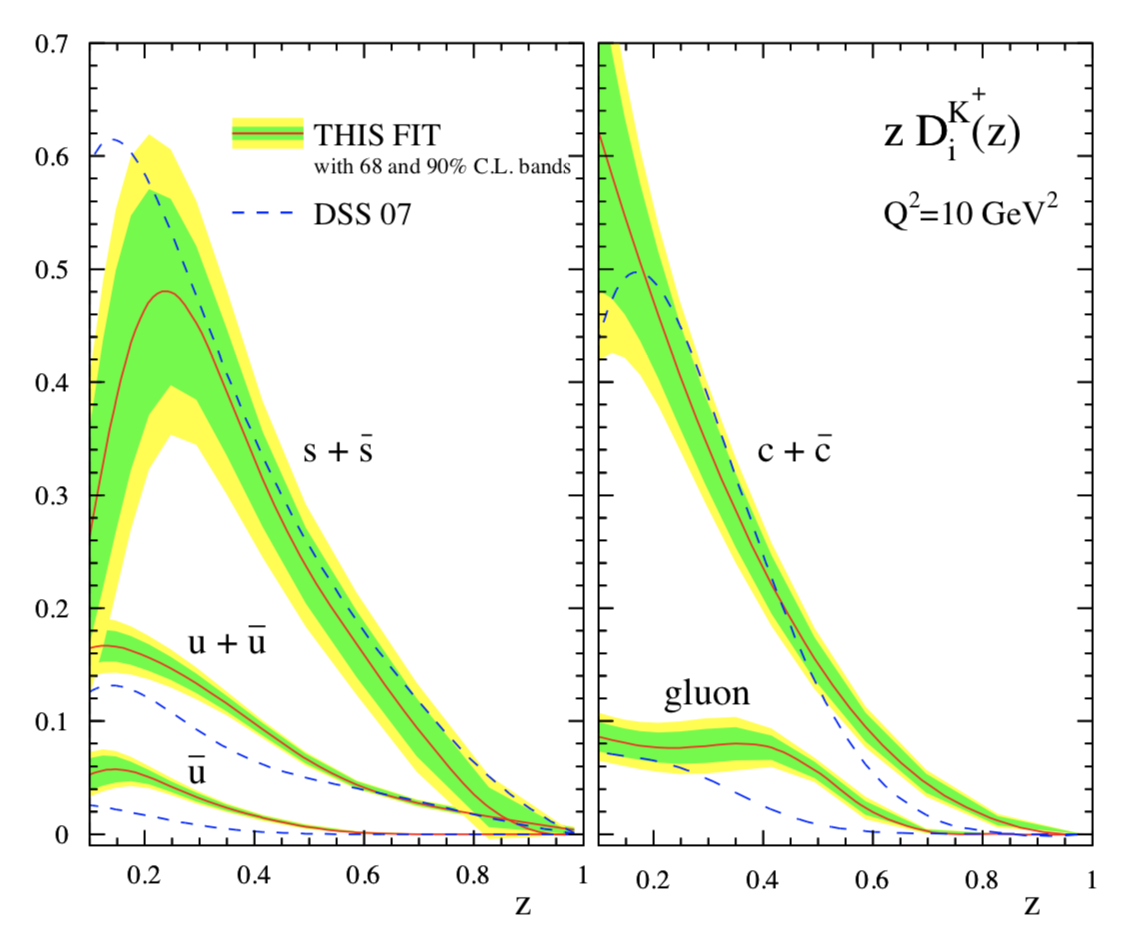
\includegraphics[scale=0.5]{./gfx/DSEHSK.png}
	\caption{Individual FFs for positively charged kaons $zD^{K^+}(z,Q^2)$ at $Q^2$ = $10$ GeV$^2$ (solid lines) along with uncertainty estimates at $68$\% and $90$\% C.L. indicated by the inner and outer shaded bands, respectively. Also shown is a comparison to previous DSS$07$ global analysis \cite{DSS07} (dashed lines). Figure taken from \cite{DSEHS2}.}
	\label{pic:DSEHSK}
\end{figure}

\subsubsection*{JAM parametrization}

JAM is a Monte-Carlo based combined fit of PDFs and FFs using Bayesian statistics. In order to address some of the questions raised by the recent ambiguities in the strange quark FFs and their impact on the $\Delta s$ determination, they go beyond the standard fitting paradigm by performing the first Monte Carlo (MC) analysis of PDFs and FFs, extending the methodology of the iterative Monte-Carlo (IMC) approach already used for the analysis of spin-dependent PDFs \cite{IMC} to the case of FFs (Fig.~\ref{pic:IMC}). The IMC approach allows for a full exploration of the parameter space using Monte-Carlo sampling together with data resampling techniques and cross validation of the fit. In consequence it reduces considerably any bias introduced by fine-tuning or fixing specific parameters that are not well constrained by the data.


\begin{figure}[!h]
  \centering
	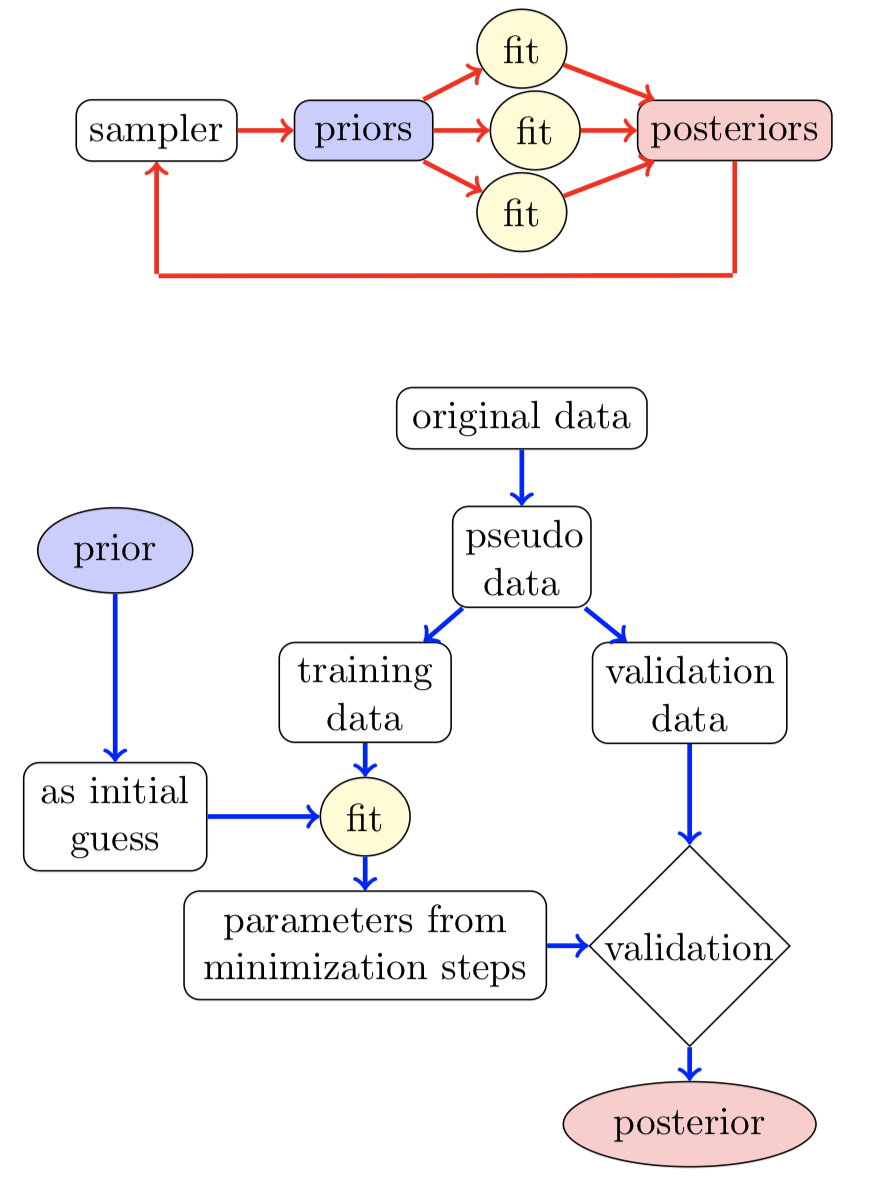
\includegraphics[scale=0.45]{./gfx/IMC.png}
	\caption{Workflow of the iterative Monte Carlo fitting strategy. In the upper diagram (red lines) an iteration begins at the prior sampler and a given number of fits are performed generating an ensemble of posteriors. After the initial iteration, with a flat sampler, the generated posteriors are used to construct a multivariate Gaussian sampler for the next iteration. The lower diagram (with blue lines) summarizes the workflow that transforms a given prior into a final posterior. Figure taken from \cite{IMC}.}
	\label{pic:IMC}
\end{figure}


The functional they use for $D^h_q$ is the following :
%
\begin{equation}
  D^h_i (z,Q_0;\textbf{a}) = M \frac{z^{\alpha}(1-z)^{\beta}}{B(2+\alpha,1+\beta)}
  \label{eq:JAMparam}
\end{equation}
%
where $\textbf{a} = {M,\alpha,\beta,\gamma}$ is the vector of shape parameters to be fitted and $B$ is the Euler beta function. The denominator is chosen so that the coefficient $M$ corresponds to the average momentum fraction $z$. Isospin symmetry is considered for all partons. Using $D^{h^{+}}_{q^{\pm}}(z,Q^2)~=~D^{h^{+}}_{q}(z,Q^2)~\pm~D^{h^{+}}_{\bar{q}}(z,Q^2)$ allows JAM to consider two templates functions for the FFs $D^{\pi^{+}}_{u^{+}}~=~D^{\pi^{+}}_{d^{+}}$, $D^{K^{+}}_{u^{+}}$ and $D^{K^{+}}_{s^{+}}$, which contain both favoured and unfavoured distributions and only one template function for the rest of unfavoured distributions viz. $D^{\pi^{+}}_{\bar{u}}~=~D^{\pi^{+}}_{d}$, $D^{\pi^{+}}_{s}~=~(1/2)D^{\pi^{+}}_{s^{+}}$, $D^{K^{+}}_{\bar{u}}~=~(1/2)D^{K^{+}}_{d^{+}}$ and $D^{K^{+}}_{s}$ along with the heavy quarks and gluons\footnote{The choice of the factor $1/2$ is motivated by data.}.

The favoured and unfavoured FFs from JAM at LO for $Q^2$ = $5$ GeV$^2$ are plotted as a function of $z$ for $\pi^+$ and $K^+$ (Fig.~\ref{pic:JAMcomp}). The strange quark fragmentation into $K^+$ from JAM$17$ is compared with DSS$07$ and HKNS results. While part of the disagreement between fits can be explained by the different parametrizations used, the large uncertainties on the data and the PDFs also play a role.

\begin{figure}[!h]
  \centering
	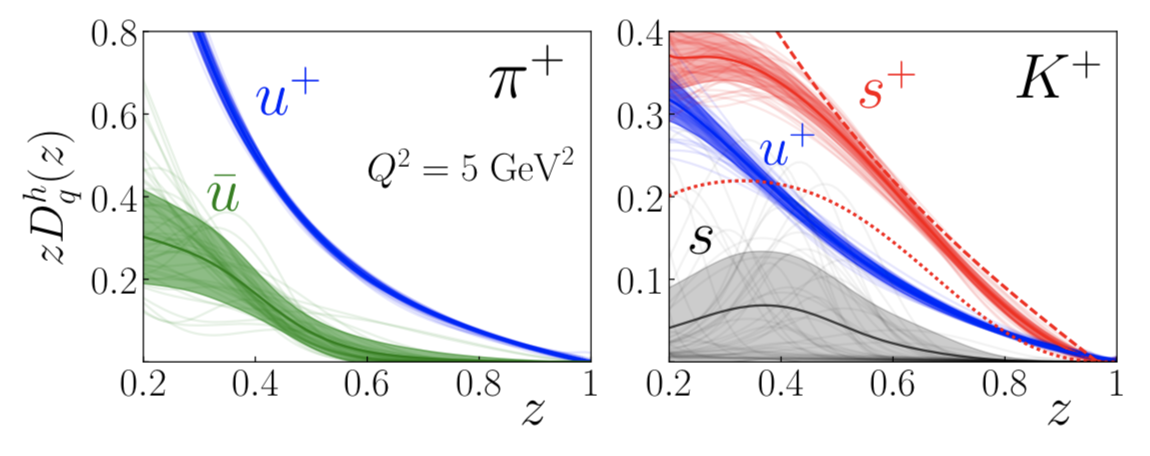
\includegraphics[scale=0.7]{./gfx/JAMcomp.png}
	\caption{Fragmentation functions $zD^h_q$ to $\pi^+$ (left panel) and $K^+$ (right panel) for $u^+$ (blue), $\bar{u}$ (green), $s^+$ (red) and $s$ (grey) at $Q^2$ = $5$ GeV$^2$ for the JAM$17$ analysis, compared to $s^+ \rightarrow K^+$ from DSS$07$ (dashed line) and HKNS (point line). Figure taken from \cite{JAM}.}
	\label{pic:JAMcomp}
\end{figure}

\section{Summary}

The DIS process is a very interesting channel for the study of the nucleon structure. The spin averaged PDFs, mostly determined from inclusive DIS, are well constrained in a wide kinematic domain for the first generation of quarks. Going to higher masses, large uncertainties still subsist e.g. for $s$ and $\bar{s}$. In SIDIS one gets additional access to FFs, which are universal quantities and parametrize quark hadronization.

Several groups have already issued parametrization of quark FFs based on LO and NLO analyses of various data sets. They differ significantly in the strange quark sector. This is why COMPASS did a new measurement and why the analysis presented in this was done.
 % Chapter 1

\cleardoublepage % Empty page before the start of the next part

%------------------------------------------------

\ctparttext{You can put some informational part preamble text here. Illo principalmente su nos. Non message \emph{occidental} angloromanic da. Debitas effortio simplificate sia se, auxiliar summarios da que, se avantiate publicationes via. Pan in terra summarios, capital interlingua se que. Al via multo esser specimen, campo responder que da. Le usate medical addresses pro, europa origine sanctificate nos se.} % Text on the Part 2 page describing the content in Part 2

\part{Analysis} % Second part of the thesis

% Chapter 2

\chapter{Renormalization and QED Radiative Corrections} % Chapter title

\label{ch:Renorm} % For referencing the chapter elsewhere, use \autoref{ch:name}

%----------------------------------------------------------------------------------------

\section{Divergences, regularization and renormalization in QED}

When calculating loop Feynman diagrams in QED at some point the integrals will diverge. To cure these divergences we have to go through the process of renormalization. Renormalization is a formal manipulation, embedded inside the quantum field theory formalism, which allows us to calculate finite testable expectation values and scattering amplitudes. However we do not know how physics decribes high energy processes : there may be high energy virtual particles contributing to the loop diagrams and they would definitely impact the divergence of the integral. Thus we could say that renormalization is a procedure allowing to calculate reasonably the effects of the low-energy physics independently to what happens at high energies.

To describe the renormalization process, consider the electron self-energy. Defining the full electron propagator $G_F(p)$ by including order-by-order in the perturbation theory the corrections to the Feynman-Green function \cite{ItzyksonZuber} :
%
\begin{equation}
    \begin{split}
      G_F(p) =
      \feynmandiagram [layered layout, horizontal=d to b] {
  b -- [anti fermion] d, };
  +
  \feynmandiagram [layered layout, horizontal=a to b]{
  a -- [anti fermion] b
  -- [anti fermion] c
  -- [anti fermion] d,
  b -- [photon, half left, looseness=1.5] c,};
  +
  \mathscr{O}(e^4_0) \\
      = \frac{i}{\slashed{p}-m_0+i\epsilon} + G^{(1)}_F(p) + \mathscr{O}(e^4_0)
    \end{split}
\end{equation}
%
where $e_0$ and $m_0$ are the \textit{bare} charge and mass parameters and $G^{(1)}_F(p)$ is a divergent term. The renormalization procedure then follows three steps :

\begin{enumerate}
  \item \textbf{Regularization} : set a new \textit{finite} integral $G^{(1)}_F(p,\Lambda)$ with a dependence with the \textit{cut-off scale}\footnote{A cut-off is often introduced in text books to explain the procedure. However, all modern practical calculations are performed with \textit{dimensional regularization}.} $\Lambda$ yielding :
  \begin{equation}
    G^{(1)}_F(p,\Lambda) \xrightarrow{\Lambda\rightarrow\infty} G^{(1)}_F(p)
  \end{equation}
  This integral has a divergent and finite part :
  \begin{equation}
    G^{(1)}_F(p,\Lambda) = I_{div}(p,\Lambda) + I_{fin}(p,\Lambda)
  \end{equation}
  The finite part $I_{fin}(p,\Lambda)$ leads to physically measurable effects and are the \textit{radiative corrections}.

  \item \textbf{Renormalization} : if the theory is \textit{renormalizable} the divergent part can be combined with the tree-level propagator :
  \begin{equation}
    \begin{split}
    G^{(1)}_F(p,\Lambda) = \frac{i}{\slashed{p}-m_0+i\epsilon} + I_{div}(p,\Lambda) + I_{fin}(p,\Lambda) + \mathscr{O}(e^4_0) \\
    = \frac{iZ_2(\Lambda)}{\slashed{p}-m(\Lambda)+i\epsilon} + I_{fin}(p,\Lambda) + \mathscr{O}(e^4_0)
    \end{split}
  \end{equation}
  Thanks to the \textit{wavefunction renormalization} $Z_2(\Lambda)$ and a renormalized mass parameter $m(\Lambda)$, the divergent terms can be integrated into the tree-level propagator.

  \item \textbf{Removing $\Lambda$-dependence} : By taking $\Lambda\rightarrow\infty$, the bare parameters $e_0$ and $m_0$ become singular allowing the physical $e$ and $m$ to be finite. The perturbation expansion is a series in $e$ and not in $e_0$.
\end{enumerate}

This procedure is well-based and defined and give consistent and definite physical results whatever regularization you choose. By definition, a theory is said to be \textit{renormalizable} if all divergences can be removed by renormalization of a finite number of parameters in the Lagrangian.

%----------------------------------------------------------------------------------------

\section{QED Radiative Corrections}

Radiative corrections had a key role in the development of QED : they enable one to calculate cross-sections with extremely high precision that has until now not been contradicted by experiment. When a process like DIS involves charged particles, there is a rearrangement of the electromagnetic current between the initial and final state. Incidentally, real photons can be emitted.

If one were to compute the cross section of the process $1+2 \rightarrow 3+4$ with no photon emission (Born level process), one would find a different result $\sigma_{0}$ than the measurement $\sigma_{exp}$. To obtain a more accurate result, one has to consider the processes $1+2 \rightarrow 3+4+\gamma_1+\gamma_2+..+\gamma_n$. Taking these corrections to Born level process into account, one obtains :
%
\begin{equation} \label{eq:RC}
  \sigma_{exp} = (1+\delta_{RC})\sigma_0,
\end{equation}
%
where $\delta_{RC}$ are the radiative corrections.


In this note, I will not discuss the corrections beyond first order. These first order corrections are also known as order $\alpha$
($o(\alpha)$) corrections. They comprise :
\begin{itemize}
\item Leptonic radiation
\item Hadronic radiation
\item Interference of lepton/hadron radiation (two-photon exchange)
\item Vacuum polarization
\item Weak corrections
\end{itemize}

The goal is to quantify the effect of radiative corrections. The observed cross-section can be expressed as the convolution of the true cross-section times a function called the radiator function which takes into account the radiative effects :
%
\begin{equation}
  d\sigma^{obs}(p,q) = \int \frac{d^{3}k}{2k^{0}}R(l,l',k)d\sigma^{true}(p,-q,k).
\end{equation}
%
A similar relation holds also for the structure functions :
%
\begin{equation}
  F_{n}^{obs}(x,Q^{2}) = \int d\tilde{x}d\tilde{Q}^{2}R_{n}(x,Q^{2},\tilde{x},\tilde{Q}^{2})F_{n}^{true}(\tilde{x},\tilde{Q}^{2}).
\end{equation}
%
The previous formulas are valid for one photon emission but can be extended to include higher-order multi-photon emissions. As one has access to both observed quantities and radiator function, the determination of the true cross-sections or structure functions from measured ones is done by unfolding using an iterative procedure. The principal drawbacks of such a method is that the solution is ill-defined : there is no unique solution, there are large uncertainties and the process is numerically unstable. To stabilize the calculation of the convolution table, i.e. the \textit{folding}, partial fractioning is used on the radiator function :
%
\begin{equation}
  R(l,l',k) = \frac{I}{k.l}+\frac{F}{k.l'}+\frac{C}{\tilde{Q}^{2}}.
\end{equation}
%
The partial fractioning is splitting the radiator function in three :
\begin{itemize}
\item Initial state radiation ($I$ fraction)
\item Final state radiation ($F$ fraction)
\item Compton peak ($C$ fraction)
\end{itemize}

For each of them, an observation can be made. For initial state radiation (ISR), $k.l$ is small for
$\angle (l_{in},\gamma) \rightarrow 0$, for final state radiation (FSR), $k.l'$ is small for
$\angle (l_{out},\gamma) \rightarrow 0$ and eventually for Compton peak $Q^{2}$ is small for
$p_{T}(l_{out}) \simeq p_{T}(\gamma)$.

For ISR and FSR, the photon is emitted within narrow cones with width of the order of $\sqrt{\frac{m_{t}}{E_{t}}}$. The radiated photon can be collinear, but it is not always collinear.
The photon can be collinear independent of whether the radiating particle has a finite mass or is massless. Collinear radiation leads to a divergence if the radiating particle is massless.

Two last notes are to be made :
\begin{itemize}
\item As $E^{2}_{\gamma,max} \propto Q^{2}\frac{1-x}{x}$, the largest radiation in energy are at large $Q^{2}$ and small $x$. Radiation is suppressed at small $Q^{2}$ and large $x$. There are also large negative corrections from uncancelled virtual contributions.
\item As $\tilde{Q}^{2}_{min} = \frac{x^{2}}{1-x}M^{2}_{N}$, the case where $\tilde{Q}^{2}_{min} \ll Q^{2}$ is possible.
\end{itemize}

All the preceding explanations did concern leptonic radiation. One should also address the question of the hadronic corrections (quark line radiation). These corrections are infrared divergent (radiation of soft photons and gluons) but they cancel with loops. The emission of the photon/gluon can be collinear and gives rise to correction of type $\frac{\alpha}{2\pi}log(m_{q}^{2})$. For quarks, the approximation $m_{q} \approx 0$ is giving rise to divergent corrections. One way to solve this issue is to factorize and absorb the divergences into the PDFs :
%
\begin{equation}
  d\sigma = \sum_{f}d\hat{\sigma}_{f}(1+\delta_{f}(Q^{2},m^{2}_{q}))q_{f}(x) = \sum_{f}d\hat{\sigma}_{f}\hat{q}_{f}(x,Q^{2}).
\end{equation}

\subsection{Characterization and impact of radiative corrections in analysis}

In the following, only DIS/SIDIS is considered.

The description of a radiative event is given by the following : an event is called radiative as soon as it contains one real radiated photon which is emitted in the lepton line (Fig. \ref{fig:rad_evt}).

\begin{figure}[htb]
\centering
\begin{tikzpicture} \begin{feynman}
\vertex (i1) {\(l\)};
\vertex[right=1cm of i1] (i3);
\vertex[above right=1cm of i3] (i4) {\(\gamma\)};
\vertex[right=1cm of i3] (a);
\vertex[above right=2cm of a] (i2) {\(l'\)};
\vertex[blob,below=2cm of a] (b) {};
\vertex[below left=2cm of b] (f12) {\(N\)};
\vertex[below=0.1cm of f12] (f13);
\vertex[above=0.1cm of f12] (f11);
\vertex[right=2cm of b] (f22);
\vertex[below=0.3cm of f22] (f23);
\vertex[above=0.3cm of f22] (f21);

\diagram* { (i1) -- [fermion] (i3) -- [fermion] (a) -- [fermion] (i2),
(i3) -- [photon] (i4),
(a) -- [photon, edge label=\(\gamma^*\)] (b) [blob],
(f12) -- [double distance=7pt] (b) [blob] -- [plain] (f22),
(f12) -- [fermion] (b) [blob],
(b) [blob] -- [plain] (f21),
(b) [blob] -- [plain] (f23),
};
\draw [decoration={brace}, decorate] (f21.north east) -- (f23.south east) node [pos=0.5, right] {\(X\)};
\end{feynman} \end{tikzpicture}
\caption{Typical Feynman diagram of a radiative event. One can note that the pair $(Q^2,\nu)$ at the vertex (called hadronic) is not the same as the one calculated using the incoming and outgoing lepton (called leptonic). The relation between the two pairs is drawn by : $\nu_{had} = \nu_{lep} - E_\gamma, Q^2_{had}=Q^2_{lep}+2E_\gamma(\nu_{lep} \sqrt{\nu_{lep}^2+Q^2_{lep}}cos\theta_\gamma)$}
\label{fig:rad_evt}
\end{figure}


In the following, we will only consider these corrections (Fig. \ref{fig:rad_dia}) :
\begin{itemize}
\item Internal Bremsstrahlung (from both incoming and outgoing leptons) (b,c)
\item Vertex correction (d)
\item Vacuum polarization (e)
\end{itemize}

\begin{figure}[htb]
\centerline{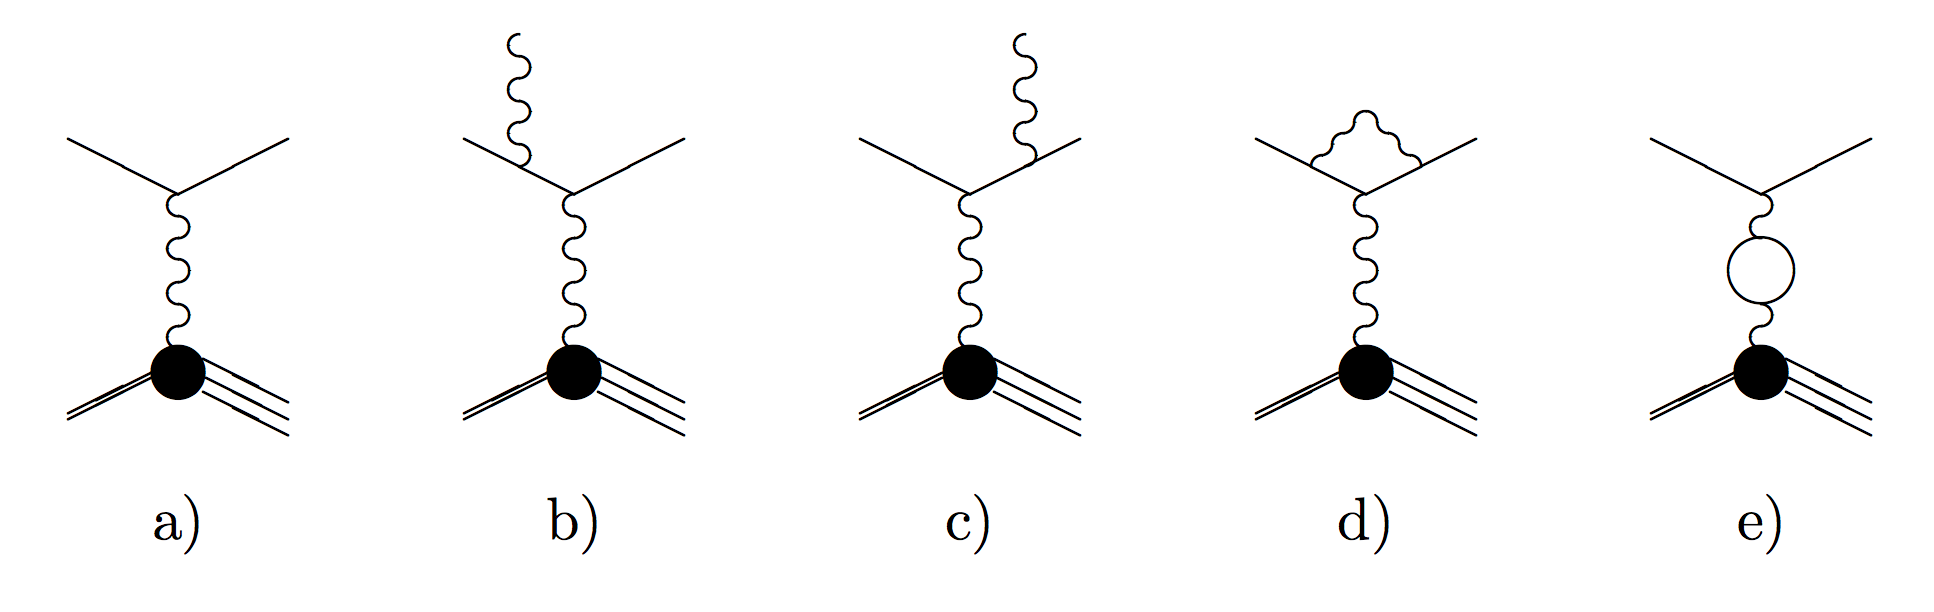
\epsfig{file=gfx/all_rad_feynm.png,width=12cm}}
\caption{List of the diagrams used for the calculation of the radiative corrections. From left to right, tree level, internal bremsstrahlung (incoming and outgoing leptons), vertex correction and vacuum polarization.}\label{fig:rad_dia}
\end{figure}

Correction to the quark line are not included in calculations, as explained in Section \ref{sec:RCF}. If we call $\sigma_{Born}$ the cross-section of the tree-level diagram and $\sigma_{Born+o(\alpha)}$ the cross-section of tree-level plus the first order correction enumerated above, the definition of the radiative corrections factor $\eta$ is :

\begin{equation} \label{eq:RCF_def}
  \eta(x,y)=\frac{\sigma_{Born}(x,y)}{\sigma_{Born+o(\alpha)}(x,y)}
\end{equation}

Obviously, the emission of a real photon is modifying the kinematic variables of the event. Let us take the case of one DIS event and a second one which is exactly like the first one except there is an ISR. The two events will share the same leptonic variables but they will have different hadronic variables. In the case of multiplicities, this discrepancy in the kinematic variables induces that some hadrons are falling into the wrong (x,y) bin. Applying the correction factor $\eta$ to the multiplicities is redirecting the hadrons to the right (x,y) bins.

\subsection{About emission of radiative photons}

There are two privileged angles (Fig. \ref{fig:plan}) for emission of a real photon :
\begin{itemize}
\item One in the direction of the incident lepton (s-peak)
\item One in the direction of the outgoing lepton (p-peak)
\end{itemize}

\begin{figure}[h!]
\centering
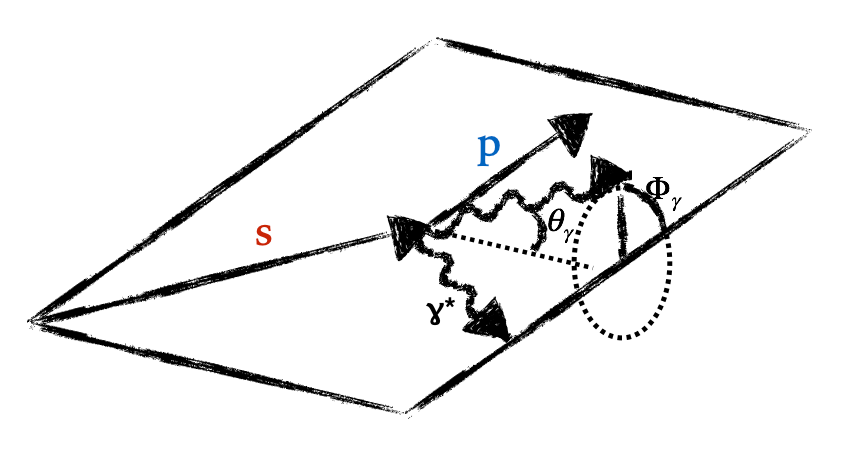
\includegraphics[width=12cm]{gfx/plan_angle.png}
\caption{Angles characterizing the emission of a radiative photon. The plane is defined by the incoming lepton (s) and the outgoing lepton (p). $\theta_\gamma$ is the polar angle and $\Phi_\gamma$ the azimuthal angle. Figure taken from \cite{TERAD2}.}
\label{fig:plan}
\end{figure}

In the case of muons, note that the $s$ and $p$ peaks are much less pronounced than for electrons.

This knowledge will later be useful to verify the consistency of DJANGOH results.

\subsection{About the radiative tail}

During elastic events, radiation of a real photon can still happen, modifying the leptonic variables of the events : this is the radiative tail. With Fig. \ref{fig:peaks}, we can see that even if we measure DIS events i.e. $Q^2$ $>$ 1, we still need informations on structure functions down to $Q^2$ = 0.

\begin{figure}[h!]
\centering
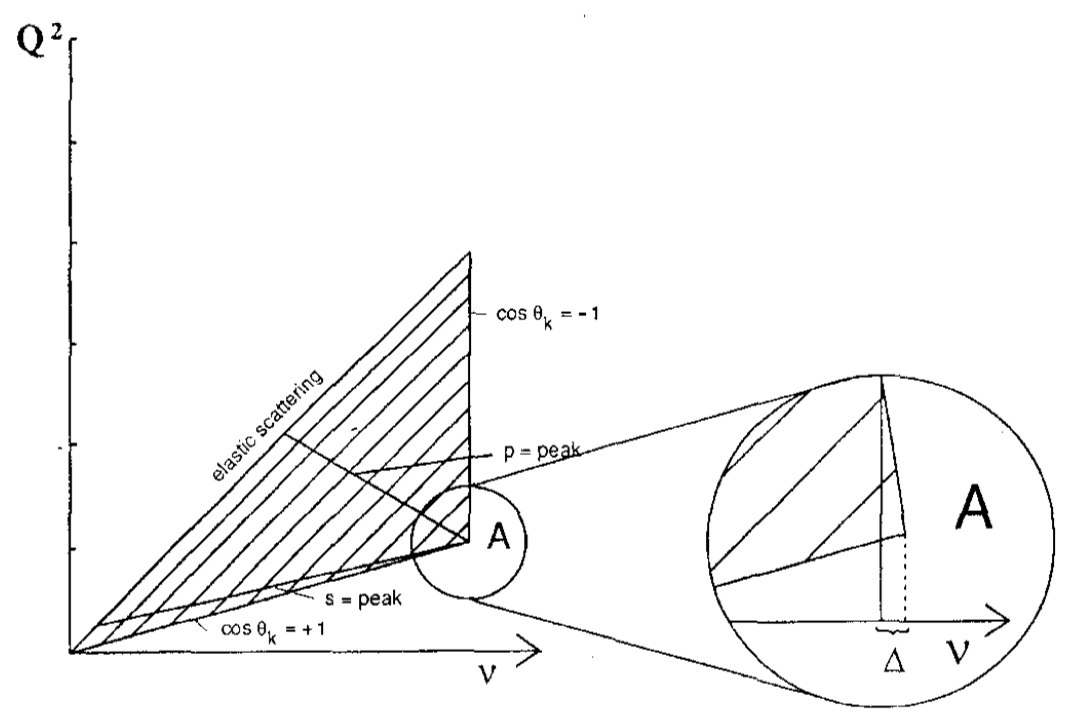
\includegraphics[width=12cm]{gfx/peaks.png}
\caption{Range of kinematical variables from which the radiative tails contribute to the cross section
measured at the point $A(Q^2, \nu)$. The s-peak is located near the boundary $cos\theta_\gamma=1$ which means
$\theta_\gamma \equiv 0[2\pi]$, thus collinear to the incoming lepton. The parallel lines are for constant $W$. Figure taken from \cite{TERAD2}.}
\label{fig:peaks}
\end{figure}

\newpage

%----------------------------------------------------------------------------------------

\section{Summary}

The renormalization is a necessary procedure when it comes to compute cross-sections as it allows to cure the divergences from the calculation and gives consistant results when compared to measurements. From this renormalization procedure arise radiative corrections which imply the emission of a real photon in the final state. These corrections can be splitted in three groups : from the Initial State Radiation (ISR), from the Final State Radiation (FSR) and from the Compton Peak. The emission of a real photon implies that there is a difference between the hadronic and leptonic variables that must be taken into account. Radiative correction factor are computed to measure the effect of the kinematic bin migration and correct the data accordingly.
 % Chapter 2
% Chapter 3

\chapter{The COMPASS experiment at CERN} % Chapter title

\label{ch:exp} % For referencing the chapter elsewhere, use \autoref{ch:name}

In this chapter a description of the COMPASS experiment is provided. The general features of the spectrometer are given in Section~\ref{sec:specgen}. The beam and target are presented in Section~\ref{sec:beam}. The descriptions of the detectors used for the tracking and the ones used for the particle identification are respectively done in Section~\ref{sec:track}. The trigger system is discussed in Section~\ref{sec:trigger}. Eventually the last sections deal with data acquisition and reconstruction.

%----------------------------------------------------------------------------------------

\section{General Overview}\label{sec:specgen}

COMPASS is a high energy, high rate fixed-target experiment at the Super Proton Synchrotron (SPS) at CERN. It is dedicated to the study of hadron structure and hadron spectroscopy with high intensity muon and hadron beams.

In order to cover the necessary large range in $Q^2$ and $x$ for the available beam energy the COMPASS spectrometer as shown in Fig.~\ref{pic:apparatus} covers a large in particle momentum and angle. Such range is obtained with a wide trigger coverage.

The apparatus is divided in three parts : the first part is dedicated to the detection of the incoming beam and is located upstream the target location. The second and third part are located downstream of the target and represent a length of $50$ meters. The second part called the \textit{Large Angle Spectrometer} (LAS) is built around the magnet SM$1$.
The LAS has been designed to provide a $180$ mrad acceptance. The \textit{Small Angle Spectrometer} (SAS), built around the magnet SM$2$, measures the particles emitted at small angles ($\pm$ $30$ mrad).

In $2016$, the data taking was performed with a $160$ Gev/c muon beam scattering off a liquid H$_2$ target.

\begin{sidewaysfigure}[!p]
  \centering
	\subfloat[LAS]{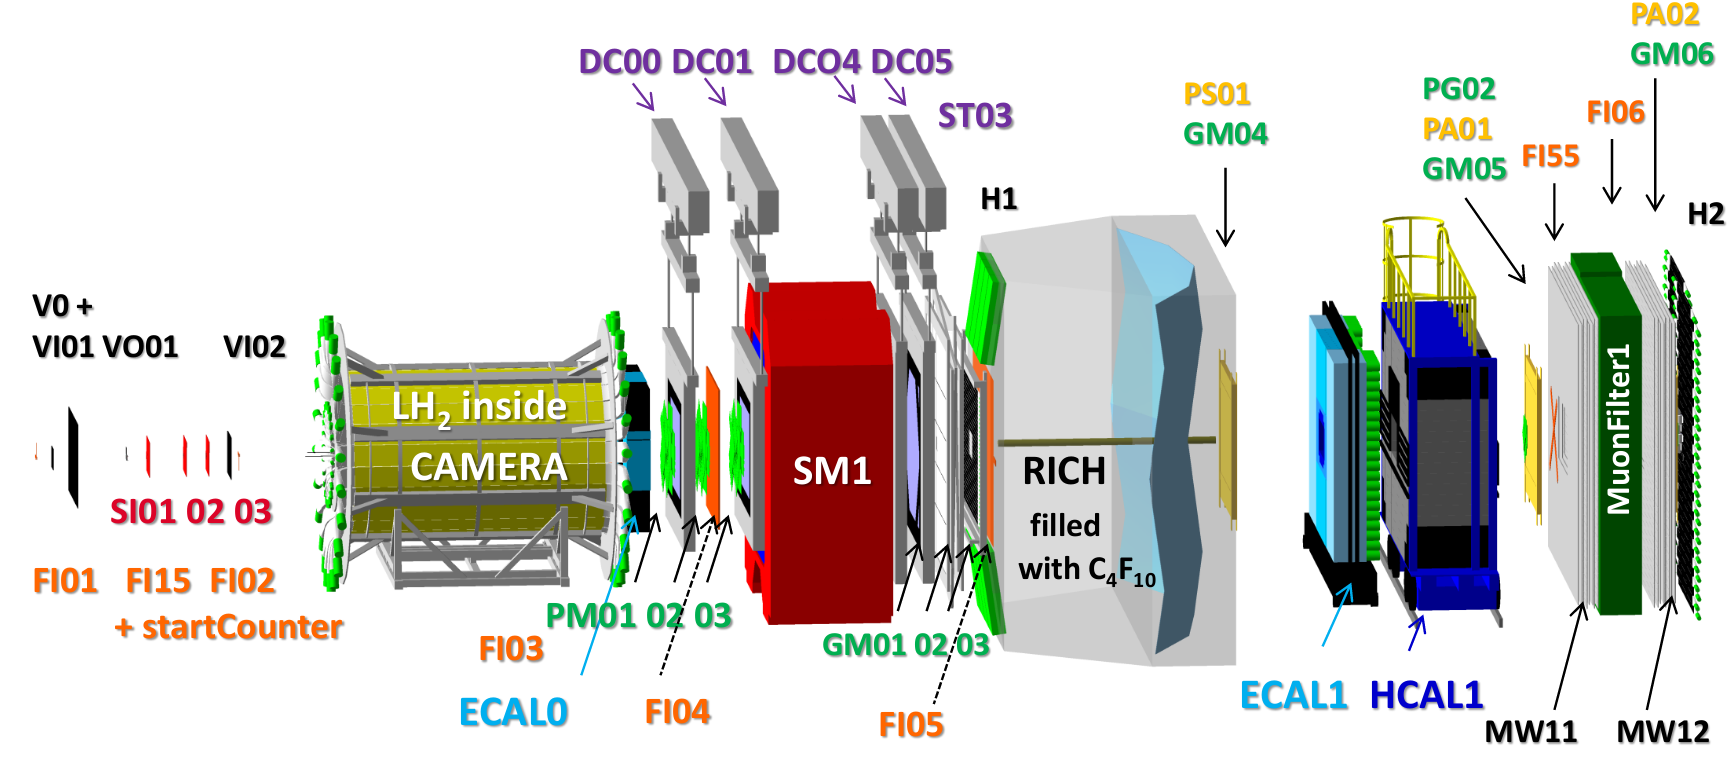
\includegraphics[scale=0.28]{./gfx/Apparatus1.png}}
  \subfloat[SAS]{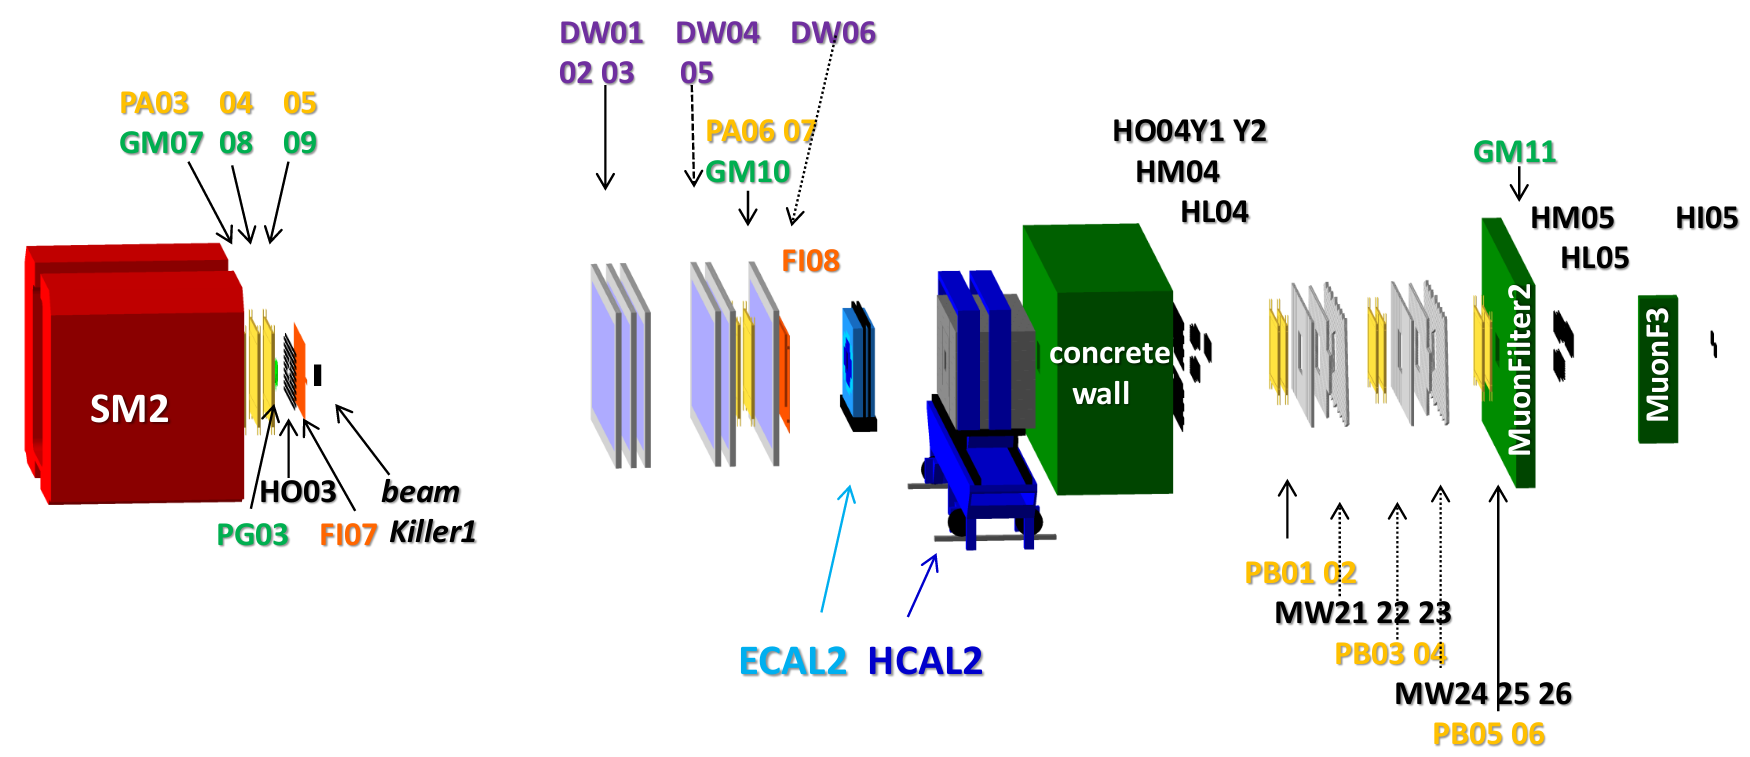
\includegraphics[scale=0.28]{./gfx/Apparatus2.png}}
	\caption{COMPASS 2016/2017 muon setup side view. Taken from \cite{Setup}.}
	\label{pic:apparatus}
\end{sidewaysfigure}

%----------------------------------------------------------------------------------------

\section{Beam}\label{sec:beam}

The muon beam used by COMPASS is obtained from a primary proton beam accelerated in the SPS up to $400$ GeV/c. The proton beam interacts with T6 target, a $50$ cm thick beryllium target, producing mainly pions and kaons. The spill time, which is the time period window within which the proton beam is delivered to the T6 target, is of $4.8$ s. In each cycle of $36$ s there are two spills.

\subsection{The M$2$ Beam Line}

The produced hadrons are transported in a $600$ m long channel of the M$2$ beamline \cite{NIM2015,M2Beam}. During this time, $5$\% of the pions and kaons are decaying into muons and neutrinos. At the end of this $600$ m decay section, remaining hadrons are stopped by a hadron absorber and the muons are focused. A system of magnets is then used to select and focus the muons of $160$ GeV/c.

The beam has transverse dimensions of $\sigma_x \times \sigma_y \sim 8 \times 8 $ mm$^2$ and an angular divergence of $\sigma_{\theta_x} \times \sigma_{\theta_y} \sim 0.5 \times 1 $ mrad$^2$ in the experimental area. At each spill, $2.10^8$ muons enter the experimental area. The beam is accompanied by a muon halo that extends transversely up to several meters of distance with respect to the beam line. The intensity of this halo decreases with the distance. The halo near the beam line as measured by a $30 \times 30$ cm$^2$ dedicated veto counter with a 4 cm diameter central hole represents $\sim$ 16\% of the muon beam. The far halo or low intensity halo is measured by a large veto counter with a central hole of $30 \times 30$ cm$^2$. It represents $\sim$ 7\% of the muon beam.

\subsection{The Beam Momentum Station}

The Beam Momentum Station (BMS) illustrated in Fig.~\ref{pic:BMS} is used for the determination of the incident muon momentum. It consists of six scintillators hodoscopes (BM$01$-BM$06$) located asymmetrically upstream and downstream a bending magnet (B$6$ : three consecutive dipole magnets) surrounded by four quadrupoles (Q$29$-Q$32$).

The BMS system was designed to measure the momentum of more than $10^8$ individual particles per spill with a relative precision of $0.5$\%. To eliminate the ambiguities in the reconstruction of particle trajectories, their time of transit is measured with a resolution of $50$~ps.

\begin{figure}[!h]
  \centering
	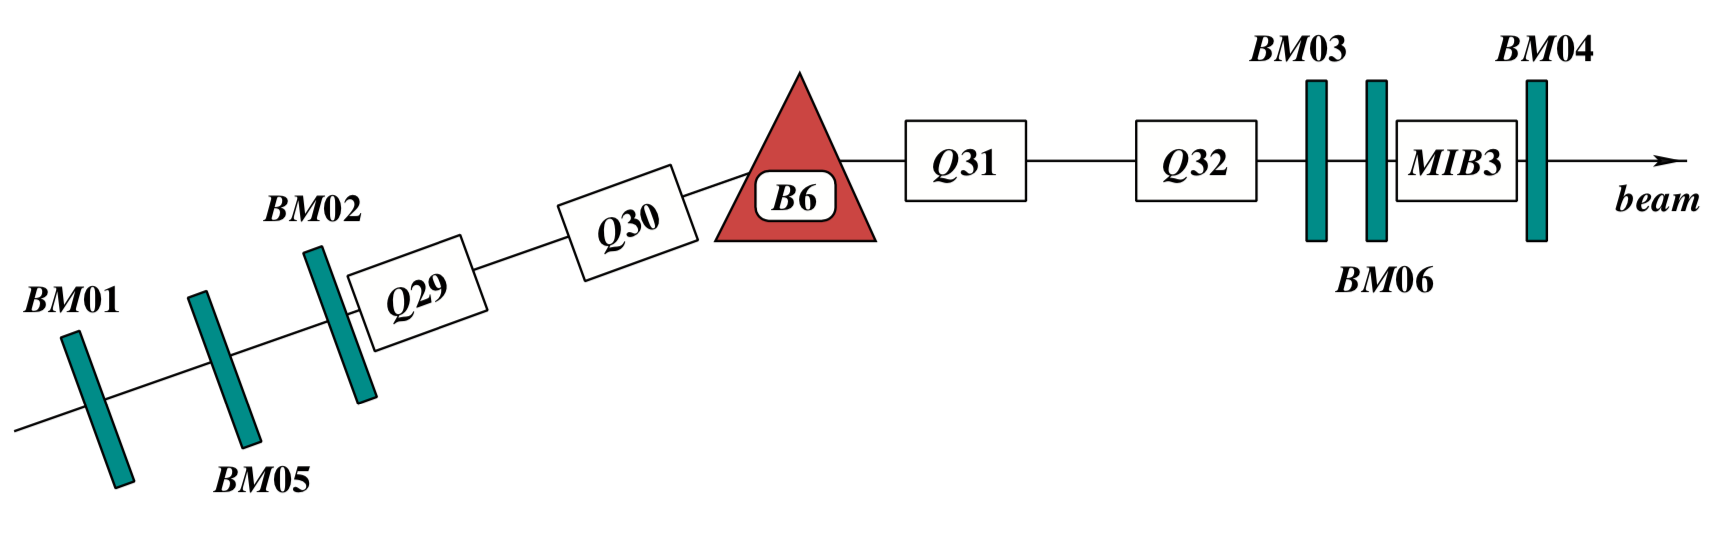
\includegraphics[scale=0.5]{./gfx/BMS.png}
	\caption{Layout of the Beam Momentum Station for the COMPASS muon beam. Taken from \cite{NIM}.}
	\label{pic:BMS}
\end{figure}

%----------------------------------------------------------------------------------------

\section{Target}

\begin{figure}[!h]
  \centering
	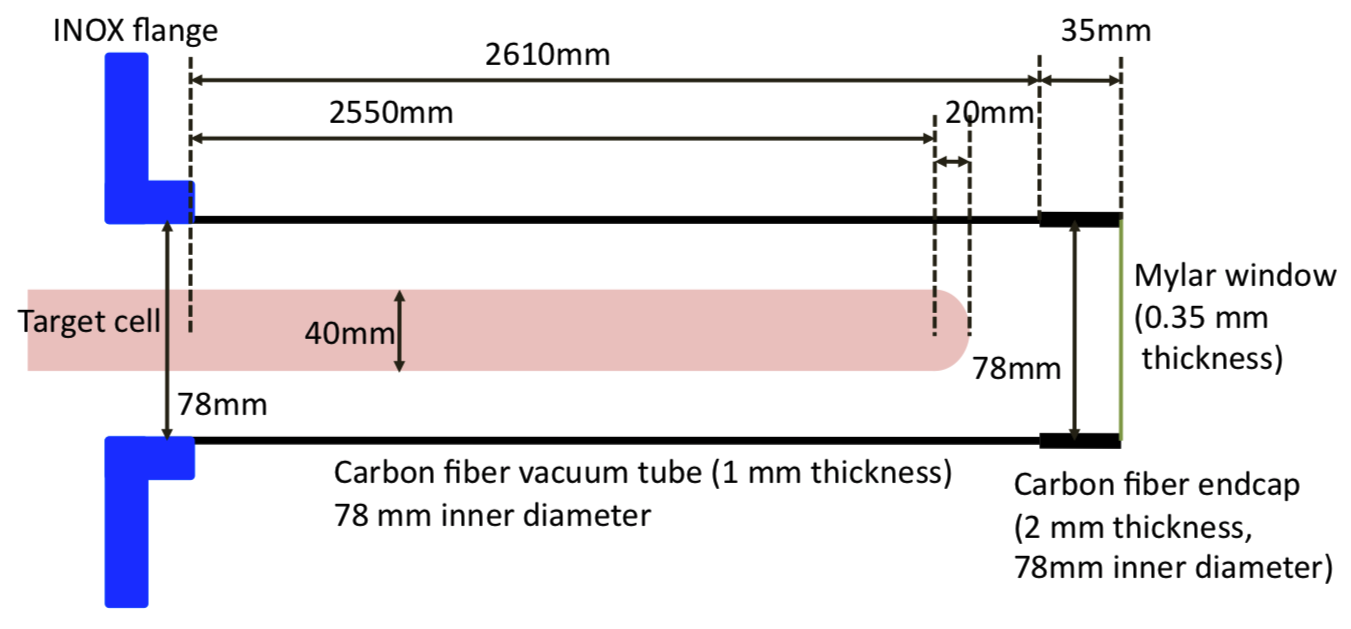
\includegraphics[scale=0.3]{./gfx/Target.png}
	\caption{Target geometry for the 2016/2017 setup.}
	\label{pic:Target}
\end{figure}

The target is liquid $H_2$ contained in a $2.5$ meter long cylinder with a radius of $2$ cm and contains lH$_2$ (Fig. \ref{pic:Target}). The target material is contained in a mylar tube with a diameter of $4$ cm. The total volume of the target cell and the liquid hydrogen system is located in a cryostat made of carbon fiber. The operation temperature of hydrogen is $18$ K with a pressure of $1020$ mbar. The material for the target cell were chosen in order to maximise acceptance.

%----------------------------------------------------------------------------------------

\section{Tracking Detectors}\label{sec:track}

The \textit{Large Angle Spectrometer} (LAS) and \textit{Small Angle Spectrometer} (SAS) are each equipped with different type of tracking detectors. Depending on the direction coverage area of each detectors they are classified as :
\textit{very small area trackers}, \textit{small area trackers} and \textit{large area trakers}

\subsection{Very small area trackers}

The very small area trackers cover the transverse beam size up to $\sim$ $3$ cm. In this region the particle rate is very high ($10^5$/s/mm$^2$ in the center of the muon beam), hence the tracking detectors must have an excellent time and position resolutions.

The scintillating fibre detectors are used at several locations of the experiment and cover areas between $\sim$ $16$ cm$^2$ and $144$ cm$^2$. They are fabricated from $0.5$-$1$ mm diameter fibres and reach a time resolution better than $500$ ps. All along the apparatus there are $9$ stations composed by two or three scintillating fiber detectors. The third detector is always pivoted by $45$° with respect to the others.

The silicon detector size is $5$x$7$ cm$^2$ with a space and time resolution of $\sim$ $10$ $\mu$m and $<$~$2.5$~ns. The $3$ silicon detectors stations are located upstream the target. The stations are each composed by two silicon detectors, the second one being rotated by $5$° with respect to the other, each detector measuring perpendicular views.

\subsection{Small area trackers}

The radial region between $2.5$ cm and $20$ cm is covered by two types of gaseous detectors : Micromegas (MICRO MEsh GAseous Structure) and GEM (Gas Electron Multiplier) detectors. These detector have a high rate capability ($\sim$ $10^4$/s/mm$^2$) and good spatial resolution ($<$ $100$ $\mu$m). They also present a minimal material budget.

The principle of the Micromegas is explained in Fig.~\ref{pic:MM}. The particle ionizes the gas in the conversion gap, the produced electrons drift in a moderate field of $1.5$ kV/cm to prevent secondary ionization, towards the amplification gap. The field in the amplification zone is large enough to accelerate the electrons to produce an avalanche. The conversion and amplification gaps are separated by a \textit{micromesh}, which collects the positive ions produced during the avalanche in a short period of time ($<$ $100$ ns). This feature is possible because of the small width of the gap ($\sim$ $100$ $\mu$m). All Micromegas detectors operate with a detection efficiency of $98$\% and with a spatial resolution of better than $100$ $\mu$m. There are three Micromegas stations located at LAS. They are composed by four detectors each with different directions : horizontal (X), vertical (Y), and two (U,V) rotated by $\pm$ $45$° with respect to the vertical. Each plane has an active area of $40 \times 40$ cm$^2$ with a deactivated central zone of $5$ cm diameter.

\begin{figure}[!h]
  \centering
	\subfloat[]{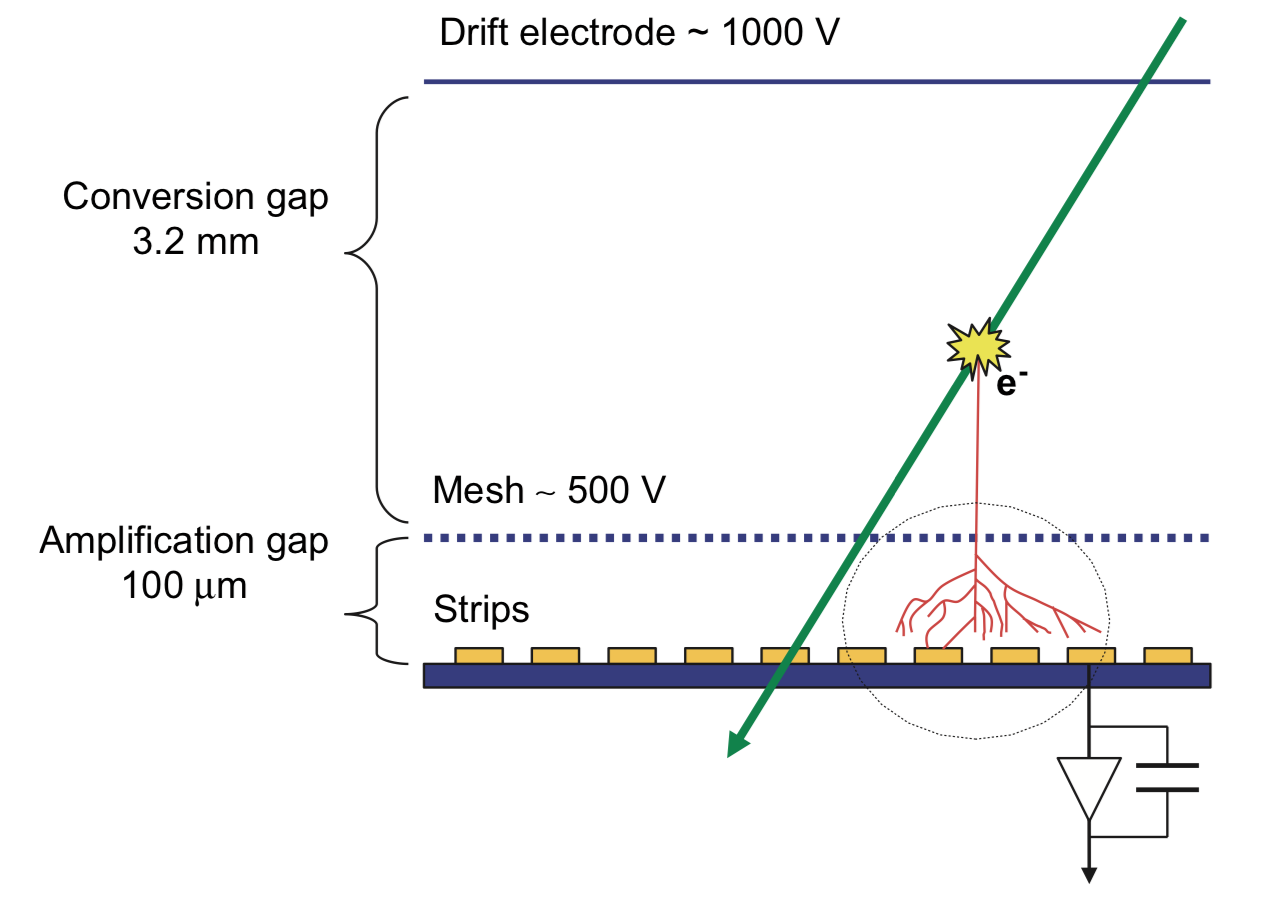
\includegraphics[scale=0.35]{./gfx/MM1.png}}
  \subfloat[]{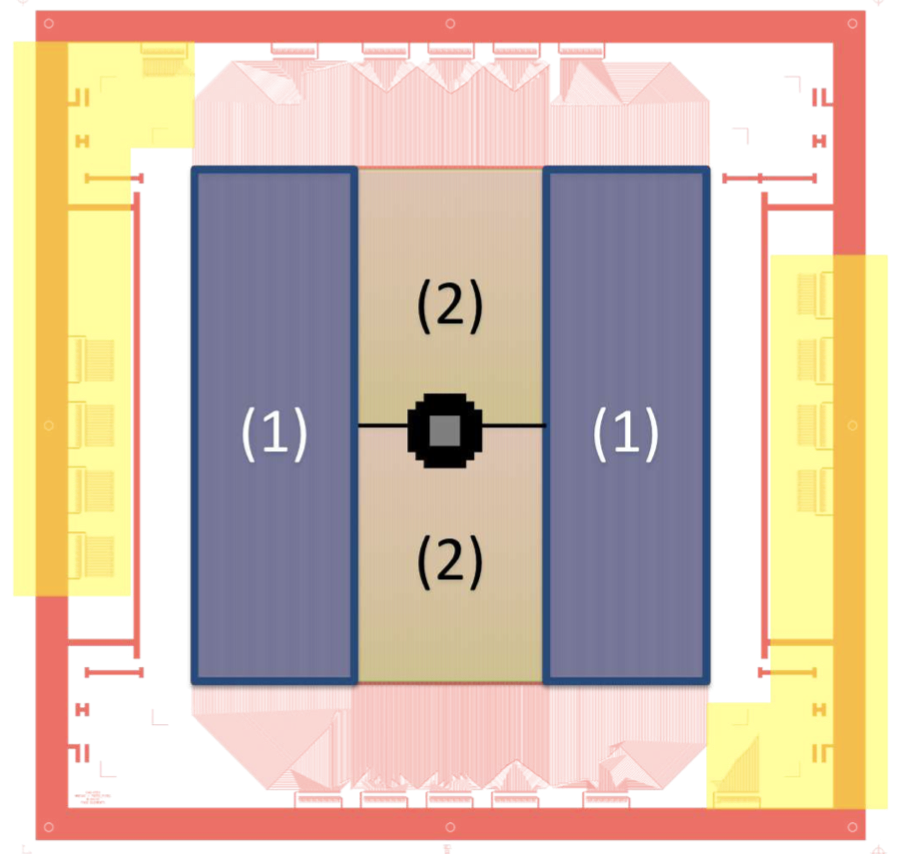
\includegraphics[scale=0.35]{./gfx/MM2.png}}
	\caption{(a) COMPASS MicroMegas detection principle. (b) MicroMegas detector. Taken from \cite{NIM}.}
	\label{pic:MM}
\end{figure}

A GEM is a $50$ $\mu$m thin polyimide foil with Cu cladding on both sides, into which numerous microholes ($\sim$ $10^4$/cm$^2$) with a diameter of $70$ $\mu$m have been chemically etched using lithographic techniques. This allows to limit gain per stage and still have high efficiencies. A high voltage (several $100$ V) is applied to each foil to generate the avalanche multiplication of the electron through the holes. The fast signal is induced by the electron cloud emerging from the last GEM foil on an anode segmented into two sets of $768$ orthogonal strips (pitch of $400$ $\mu$m). The COMPASS GEM detection principle is shown in Fig.~\ref{pic:GEM} : it consists of three GEM amplification stages separated by thin grids of $2$ mm height. A GEM station is composed by $2$ detectors oriented by $45$° relatively to each other. All in all there are $11$ stations, all located at SAS. The active area for the GEM is $31 \times 31$ cm$^2$ and the central area of $5$ cm diameter can be activated to align the detector with low intensity beams. The detectors efficiency is $\sim$ $97$\% with a spatial and time resolution of about $\sim$ $70$ $\mu$m and $12$ ns, respectively.

\begin{figure}[!h]
  \centering
	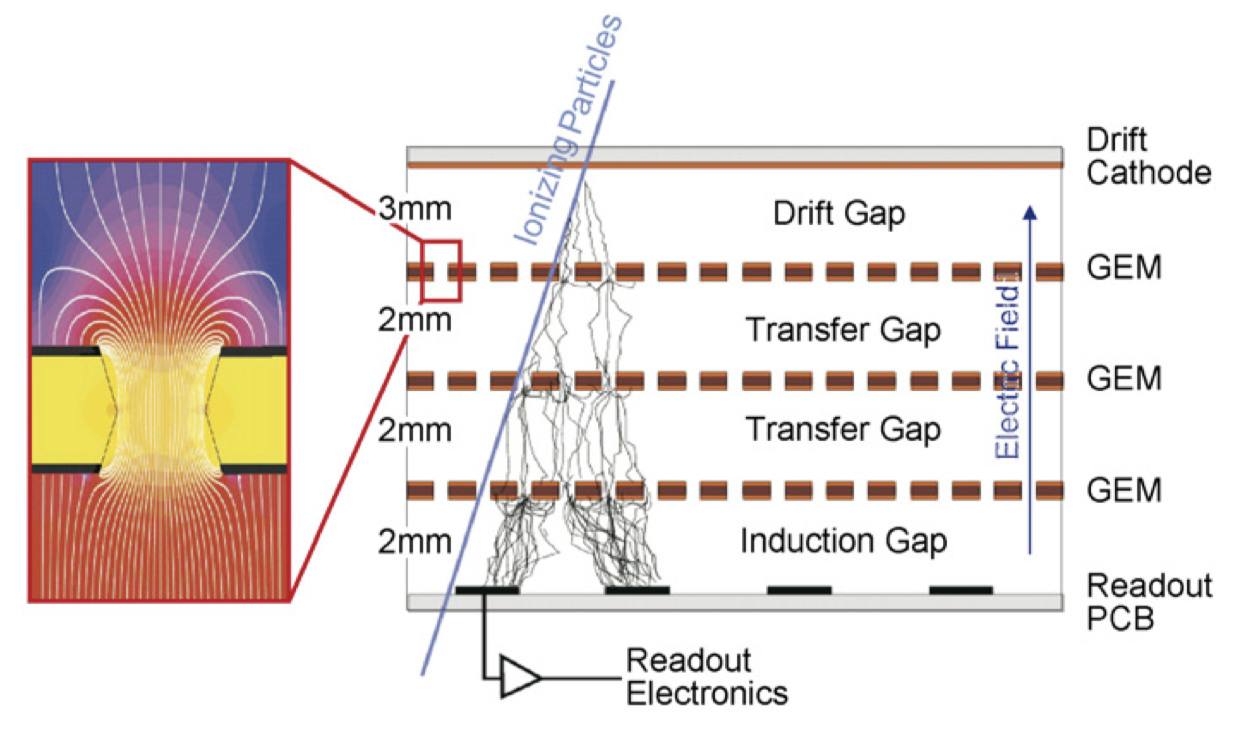
\includegraphics[scale=0.5]{./gfx/GEM.png}
	\caption{COMPASS GEM detection principle. Taken from \cite{NIM}.}
	\label{pic:GEM}
\end{figure}

\subsection{Large area trackers}

The large area trackers cover all the spectrometer acceptance with a good spatial resolution. As the particle rate in the region covered by the large area trackers is small in comparison to the central region ($10^2$/s/mm$^2$), the use of detectors such as drift chambers (DCs and W$4/5$) \cite{DaCosta}, straw drift tubes \cite{Zvyagin} and multiwire proportional chambers (MWPCs) is possible. These detectors have large active size area ($\sim$ m$^2$) with a central dead zone of few cm$^2$.

Each DC consists of eight layers of wires with four different inclinations : horizontal, vertical and rotated $\pm$ $20$° with respect to the vertical direction (X, Y, U and V). Two consecutive planes with the same inclination are staggered by $3.5$ mm to disimbiguate left-right and the ordering of the planes with different orientations is such to minimize the fake track combinations. The detectors are filled with a gas mixture of Ar, C$_2$H$_6$ and CF$_4$ at a volume ratio $9:9:2$. Two of the DC are located before SM$1$ and have an active area of $180 \times 127$ cm$^2$~; the last two are located downstream SM$1$ and have a larger active area of $204 \times 204$ cm $^2$. All these DCs have a central dead zone of $30$ cm. The central dead zone can be activated for alignment needs with a low intensity beam. The average resolution of a DC is $270$ $\mu$m and the efficiency above $95$\%.

The W$4/5$ detectors have an active area of $5$ x $2.5$ m$^2$, and consist of $4$ anode wire layers with a wire pitch of $4$ cm. The anode wires are separated by layers of cathode wires with a pitch of $2$ mm. The diameter of the anode wire is $20$ $\mu$m and of the potential wires, $200$ $\mu$m. A CF$_4$-based gas mixture, Ar/CF$_4$/CO$_2$ ($85/10/5$), is used.

A straw detector station consists in $3$ straw detectors with different orientations : horizontal, vertical and rotation by $10$° with respect to the vertical. The only station used is located between SM$1$ and SM$2$. Each detector is composed by two layers of straw tubes with the same orientation. The straw tubes consist in two layers of thin plastic film, one coated with carbon loaded Kapton, the other one with aluminised Kapton foil. The active area for the straw detector is $320 \times 280$ cm$^2$ and have a central dead zone of $20 \times 20$ cm. The average resolution is of $190$ $\mu$m.

There are three types of MWPCs in COMPASS, which differ by the number of layers, the size of the dead zone for the beam and the combination of the measured projections (X, Y, U and V). The active area is of $178 \times (90-180)$ cm$^2$. All layers have a wire length of about $1$ m, a wire diameter of $20$ $\mu$m and a pitch of $2$ mm and are enclosed on both sides by graphite-coated Mylar foils. The central deadzone of each detector increases with respect to the detector position, from $16$ to $22$ cm. The average spatial resolution of the MWPC is of $1.6$ mm.

\begin{table}[!h]
  \caption{Table with the characteristics of a selection of tracking detectors.}
  \label{tab:kinvar}
  \centering
  \begin{tabular}{c|c|c|c}
    \hline
    \hline
    Detector type & Active area & Spacial resolution & Time resolution \\
    \hline
    \hline
    Scintillating Fibre & $(3.9)^2$ - $(12.3)^2$ cm$^2$ & $130$ - $210$ $\mu$m & $400$ ps \\
    Silicon Micro-strip & $5$ x $7$ cm$^2$ & $8$ - $11$ $\mu$m & $2.5$ ns \\
    GEM & $31$ x $31$ cm$^2$ & $70$ $\mu$m & $12$ ns \\
    Micromega & $40$ x $40$ cm$^2$ & $90$ $\mu$m & $9$ ns \\
    MWPC & $178$ - $(90-120)$ cm$^2$ & $1.6$ $\mu$m & N/A \\
    DC & $180$ - $127$ cm$^2$ & $190$ - $500$ $\mu$m & N/A \\
    Straws & $280$ - $323$ cm$^2$ & $190$ $\mu$m & N/A \\
    \hline
    \hline
  \end{tabular}
\end{table}

%----------------------------------------------------------------------------------------

\section{Particle Identification}

Particle identification is performed by all the tracking detectors. A RICH detector allows to separate between pions, kaons and protons at high intensity environment. Two types of calorimeters are used to measure the energy of the hadrons, photons and electrons : hadrons calorimeters (HCAL1 and HCAL2) and electromagnetic calorimeters (ECAL1 and ECAL2). Two muon wall detectors (MW1 and MW2) are performing muon identifications and consist of tracking detectors combined with a hadron absorber. While the RICH will be further described in a dedicated chapter (Chapter~\ref{ch:PID}), the other identification detectors will be briefly described in the following subsections.

\subsection{Hadron Calorimeters}

A hadron calorimeter allows to separate hadron and muon tracks on the energy deposit. Contrary to a hadron, which deposits almost all its energy via a hadron shower, the muon suffers on energy loss by only deposit a small energy fraction. HCAL$1$ and HCAL$2$ are sampling calorimeters with a modular structure with iron and scintillator plates and are located before the muon filters. Their efficiency depends on the energy : for HCAL$1$ for hadrons with momenta above $5$ GeV/$c$ it is almost constant and close to $100$\% when for HCAL$2$ the same efficiency is reached for hadrons with momenta above $10$ GeV/$c$.

\subsection{Electromagnetic Calorimeters}

The electromagnetic calorimeters are used to measure the energy of electrons and photons. ECAL$1$ and ECAL$2$ are formed by blocks of lead glass connected to photomultipliers with light guides. An electromagnetic shower is initiated when the incoming electrons of photon reach the calorimeter. This electromagnetic shower produces Cherenkov radiation inside the lead glass and this light intensity is proportional to the energy deposited. The inner-most part of ECAL$2$ has radiation-hard Shashlyk-type lead/scintillator modules.

\subsection{Muon Identification with Muon Walls and Muon Filters}

An efficient way to identify muons is to use an absorber surrounded by two tracking detec- tors. With a radiation length large enough to absorb all hadrons, particles detected behind the absorber are considered muons. At COMPASS, this is done in the LAS with the Muon Wall $1$ (MW$1$) and the Muon Filter $1$ (MF$1$). In the SAS, the Muon Wall $2$ (MW$2$) in combination with the Muon Filter $2$ (MF$2$) identify the muons. At the very end of the spectrometer, the Muon Filter $3$ (MF$3$) is the last muon filter detector. The three muon filters are made of steel or concrete. The MW$1$ system consists of Mini Drift Tubes. The tubes are made of $0.6$ mm thick aluminum tubes surrounding a $50$ $\mu$m thick tungsten wire. The muon filter surrounded by the MW$1$ system is made of $60$ cm of steel. The active areas are $4845$ x $4050$ mm$^2$ (hole: $1445$ x $880$ mm$^2$) and $4730$ x $4165$ mm$^2$ (hole: $1475$ x $765$ mm$^2$) for the X and Y planes. The gas mixture of MW$1$ is Ar/CO$_2$ ($70/30$). The MW$2$ system in the SAS has two identical stations of layers of drift tubes. Each of the two stations consists of $6$ layers with an active area of $4470$ x $2020$ mm$^2$. A gas mixture of Ar/CH$_4$ ($75/25$) is used. The stainless steel drift tubes have an inner diameter of $29$ mm and a wall thickness of $0.5$ mm and the wires are $50$ $\mu$m thick.

%----------------------------------------------------------------------------------------

\section{The Trigger System}\label{sec:trigger}

The trigger system \cite{TriggerSys} has the task to select physic event candidates in a high rate environment. It is composed by scintillator hodoscope, complemented by scintillator veto detectors to suppress halo muons and by calorimeters to select events with hadron production. In the central region MWPCs complements the coverage of the muon acceptance.

\begin{table}[!h]
  \caption{COMPASS triggers with the muon beam in 2016.}
  \label{tab:kinvar}
  \centering
  \begin{tabularx}{7.5cm}{cc}
    \hline
    \hline
    Trigger name & Components \\
    \hline
    \hline
    Middle Trigger (MT) & HM$04$, HM$05$ \\
    Ladder Trigger (LT) & HL$04$, HL$05$ \\
    Outer Trigger (OT) & HO$03$, HO$04$ \\
    LAS Trigger (LAST) & H$1$, H$2$ \\
    \hline
    \hline
  \end{tabularx}
\end{table}

Depending on the event kinematics two different algorithms are used to determine the scattered muon kinematics. When the angle of the scattering muon is large enough ($Q^2 > 1$ (GeV/$c$)$^2$) to be measured by using only the hodoscope stations, the trigger signals are built using the vertical pointing algorithm (Fig.~\ref{pic:triglogic}).

\begin{figure}[!h]
  \centering
	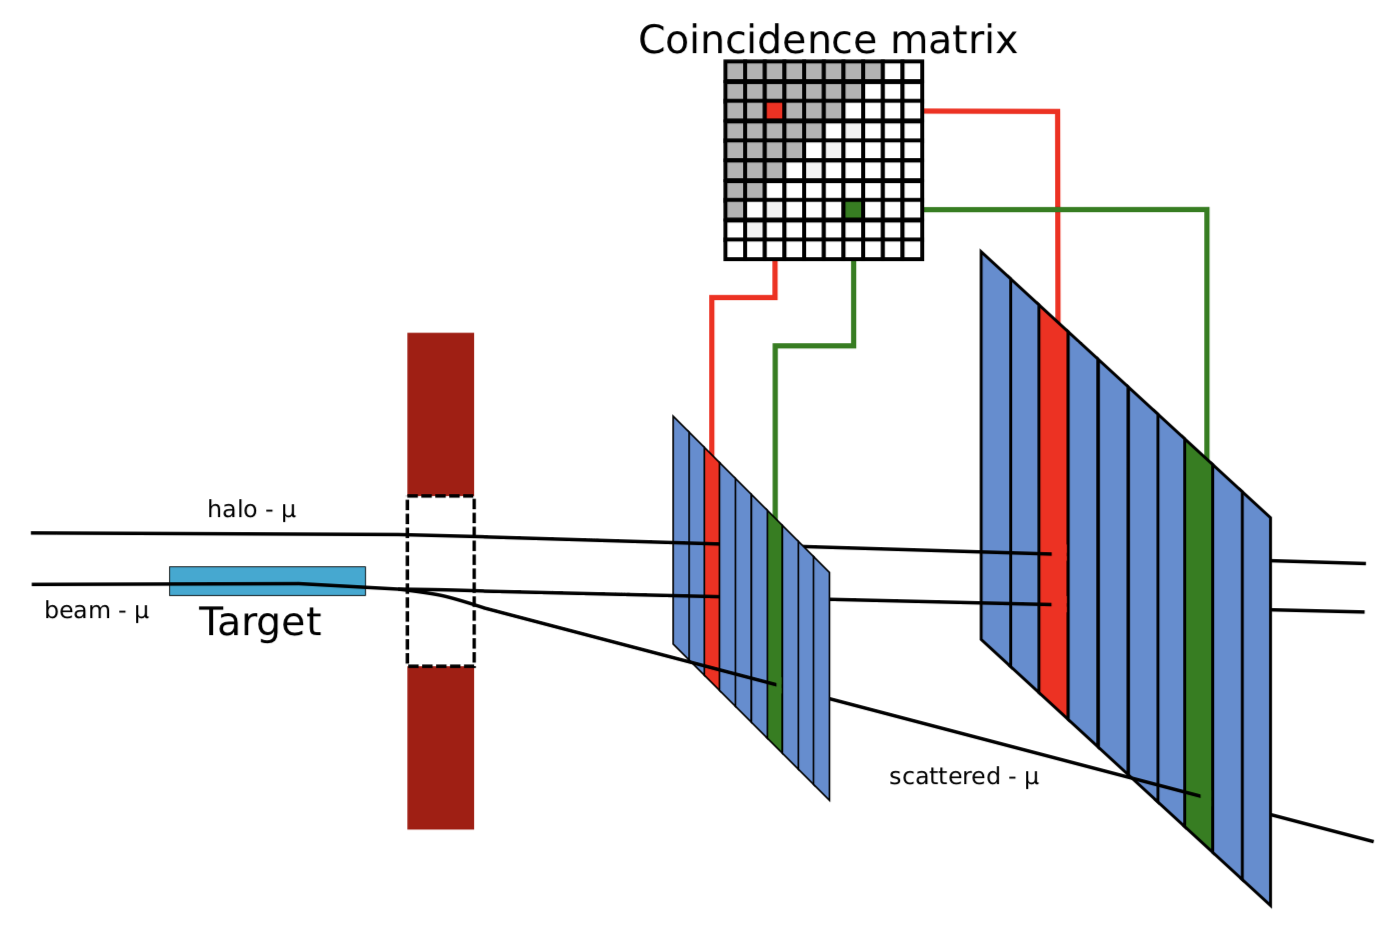
\includegraphics[scale=0.5]{./gfx/TriggerLogic.png}
	\caption{Concept of the trigger. The scattered muon leads to a coincidence in the activated area of the coincidence matrix while the halo muon fails to do so.}
	\label{pic:triglogic}
\end{figure}

The angle ($\theta_x,\theta_y$) of the scattered muon is determined by using two hodoscopes with horizontal strips located at different positions along the beam direction and the vertical component $\theta_y$ is determined. If $\theta_y$ is compatible with the target position the trigger system validates the event. The $y$-$z$ plane is selected since the particle track is not deflected by the dipole magnet in y-direction. In cases where the scattering angle of the muon is too low to be measured ($Q^2 < 1$ (GeV/$c$)$^2$), the bending angle of the magnet is used to determine $\theta_x$ and to perform an energy loss measurement to fire the trigger. This is possible since the muon energy loss $\nu$ is translated into a deflection by the magnetic dipole field.

The kinematic range covered by the trigger system is shown in Fig.~\ref{pic:trigger}. The trigger system is optimized to select DIS events. The lowest $Q^2$ events are covered by the \textit{ladder} trigger (LT) followed by \textit{middle} trigger (MT), \textit{outer} trigger (OT) and \textit{LAS} trigger (LAST) with increasing $Q^2$.

\begin{figure}[!h]
  \centering
	\subfloat[]{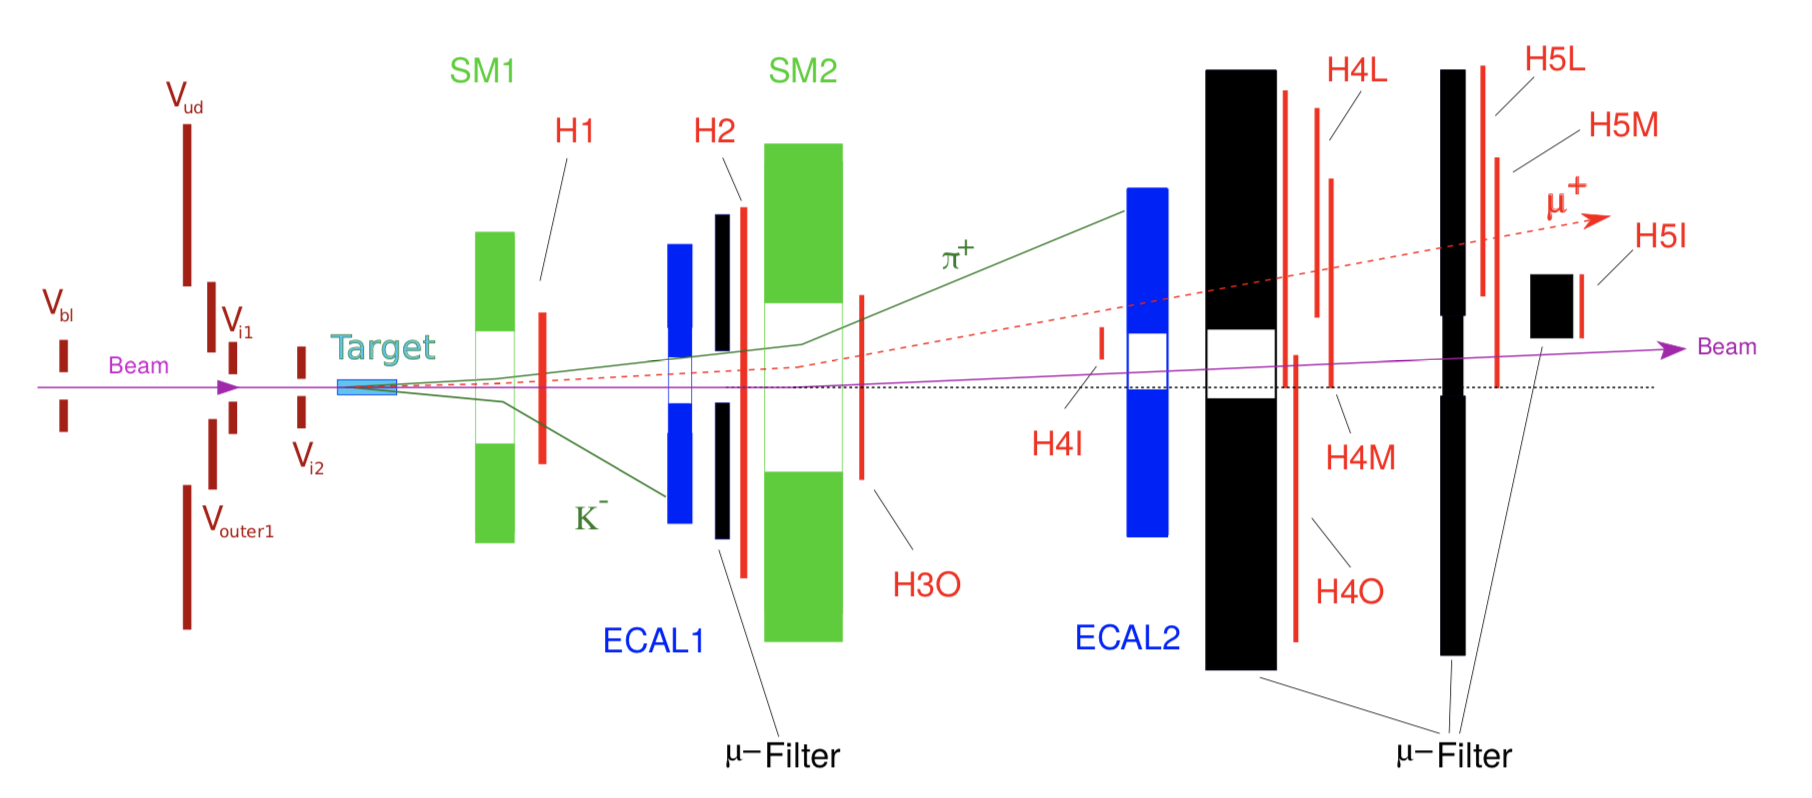
\includegraphics[scale=0.3]{./gfx/TriggerSys.png}}
  \subfloat[]{\includegraphics[scale=0.26]{./gfx/TriggerCov.png}}
	\caption{(a) Main elements of the trigger system. (b) Trigger system kinematic coverage.}
	\label{pic:trigger}
\end{figure}

%----------------------------------------------------------------------------------------

\section{Data Acquisition}

The data acquisition system (DAQ) \cite{NIM} is in charge of managing the information coming from more than $250000$ spectrometer electronic channels and building events. At COMPASS the typical event size is $45$ kB at a trigger rate of about $10$ kHz. The pipeline used in the DAQ is illustred in Fig.~\ref{pic:DAQ}. First the analog signals are coming from the detectors are preamplified, then they are digitized directly at the front-end by Analog to Digital Converters (ADCs) or Time to Digital Converters (TDCs) according to the type of detectors the front-ends are coupled to. The data are then transferred to the readout driver modules CATCH (COMPASS Accumulate, Transfer and Control Hardware) of GeSiCA (GEM and Silicon Control and Acquisition) upon the arrival of a trigger signal provided by the Trigger Control System (TCS). CATCH and GeSiCA combine the data from up to $16$ cards (ADC or TDC) and transmit them via an optical S-Link to the computers named \textit{Readout Buffer} (ROBs, maximum through output 160 MB/s) where they are stored in $512$ MB spill buffer cards. During the $4.8$ s of beam time the data are written to memory, during the rest of the full SPS cycle ($36$ s) they are read through a PCI interface. In this way the required bandwidth is reduce by a factor of three. The events are built by 12 event builders and are then written to multiple $1$ GB large files (chunks) labeled by the run number and their consecutive chunk number. Finally the data are transferred to the CERN central data recording facility (CASTOR).

\begin{figure}[!h]
  \centering
	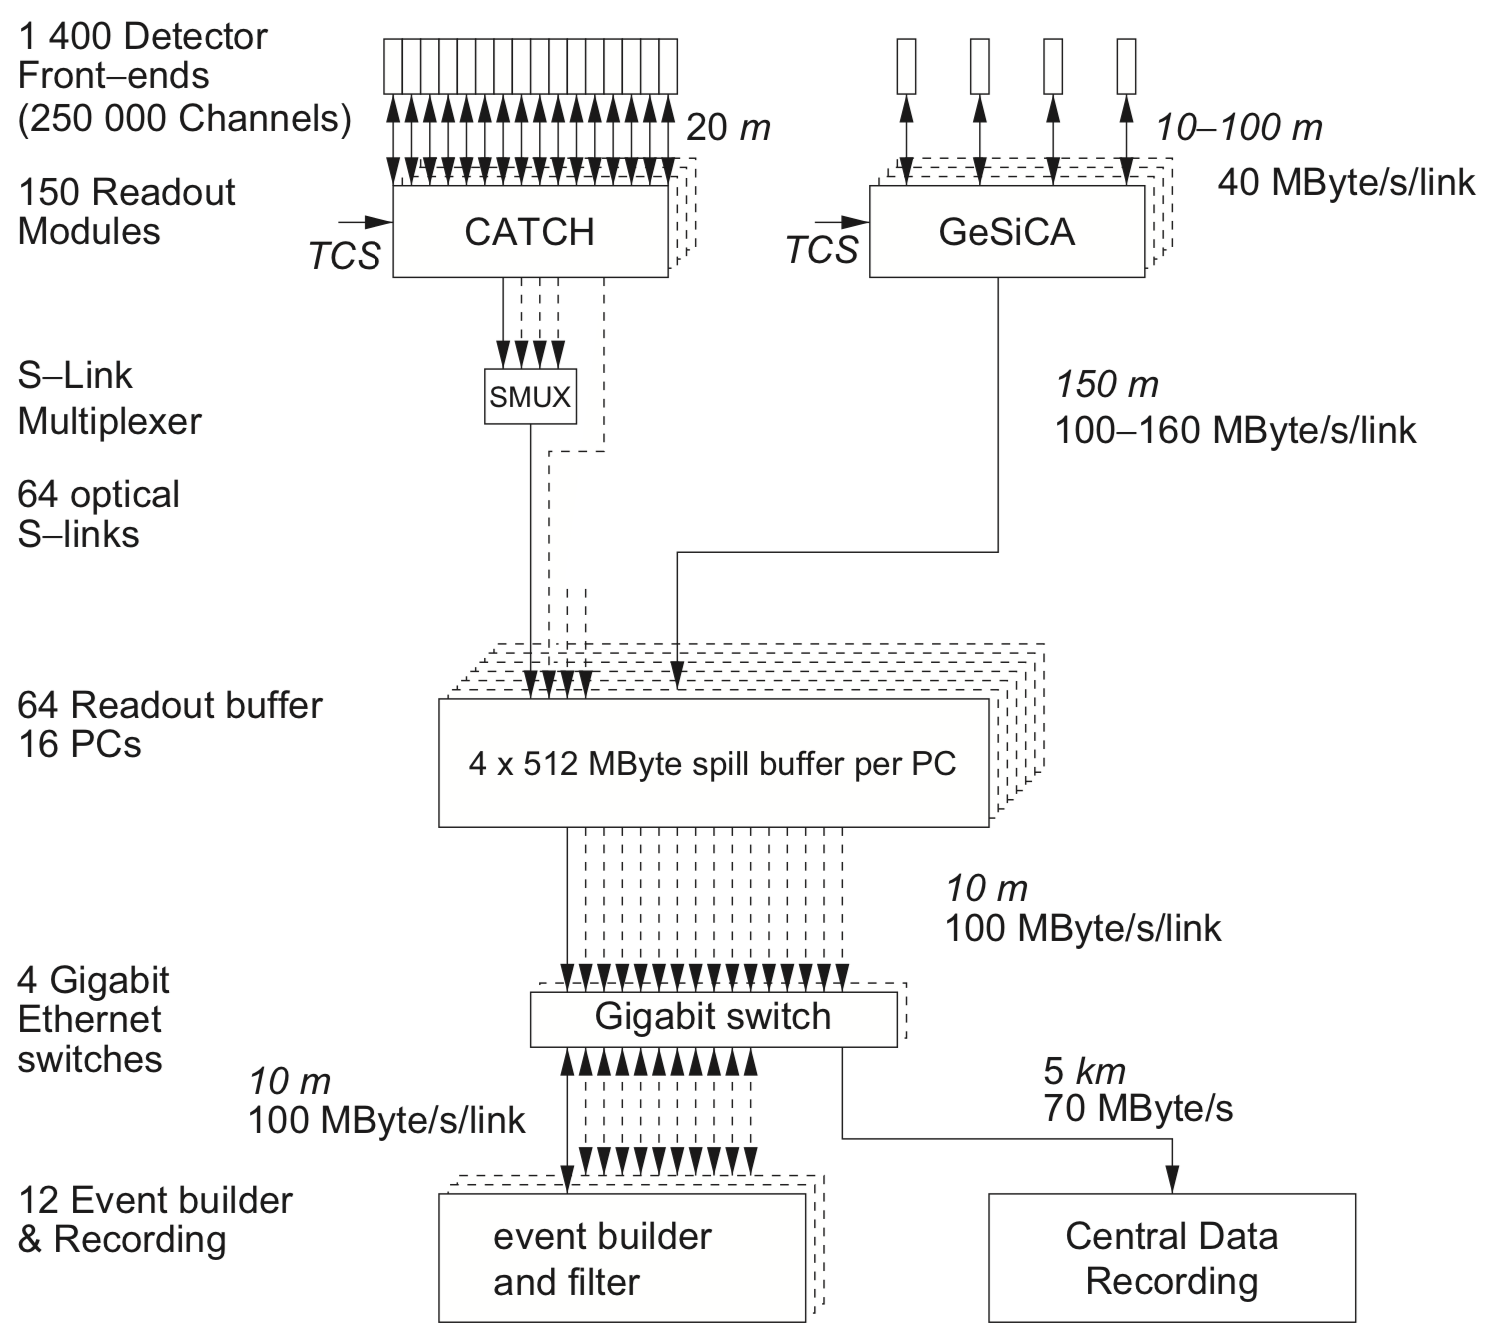
\includegraphics[scale=0.4]{./gfx/DAQ.png}
	\caption{General architecture of the DAQ system. Digitized data from the detector front-end are combined on the CATCH and GeSiCA modules. The storage of the data during the spill and the event building is performed locally. The data are recorded at the CERN computing center. Taken from \cite{NIM}.}
	\label{pic:DAQ}
\end{figure}

%----------------------------------------------------------------------------------------

\section{Event Reconstruction}

The offline reconstruction of the events stored in CASTOR is performed by the COMPASS software CORAL\footnote{COMPASS Reconstruction Algorithm Library} \cite{NIM}. CORAL is also used for the reconstruction of events generated by the Monte-Carlo simulation tool TGEANT (see Chapter~\ref{ch:MC}). CORAL is written in C++ and has a modular structure. The scheme of the steps followed by the reconstruction program is shown in Fig.~\ref{pic:CORAL}. First the information on the fired detectors channels is extracted. This is known as decoding and in the MC case digitization. In general there are more than one detector channels fired by the same particle. In that case a clustering algorithm is applied : the neighbouring detector channels that were fired are grouped together and the coordinate of the cluster in the apparatus reference system is computed. At this stage the detector calibration and position are used to extract the information. The CORAL output is stored in a ROOT Tree called mDST (mini Data Summary Tape).

The physics information is extracted from the mDST using the software package PHAST\footnote{PHysics Analysis Software Tools}. PHAST gives access to the reconstructed event information and it provides a set of algorithm to compute the relevant physics variables of each event. The PHAST outputs are stored again in a ROOT Tree. These files are significantly smaller than the mDSTs and are used for the final physics analysis.

In COMPASS, the experimental data are organized into several levels. The basic level are the events collected in one \textit{spill} provided by the SPS. A \textit{run} is the equivalent of $200$ spills. As there are machine development and/or realignment each week, the data are then structured in \textit{weeks} (also called \textit{period}) containing multiple runs.

\begin{figure}[!h]
  \centering
	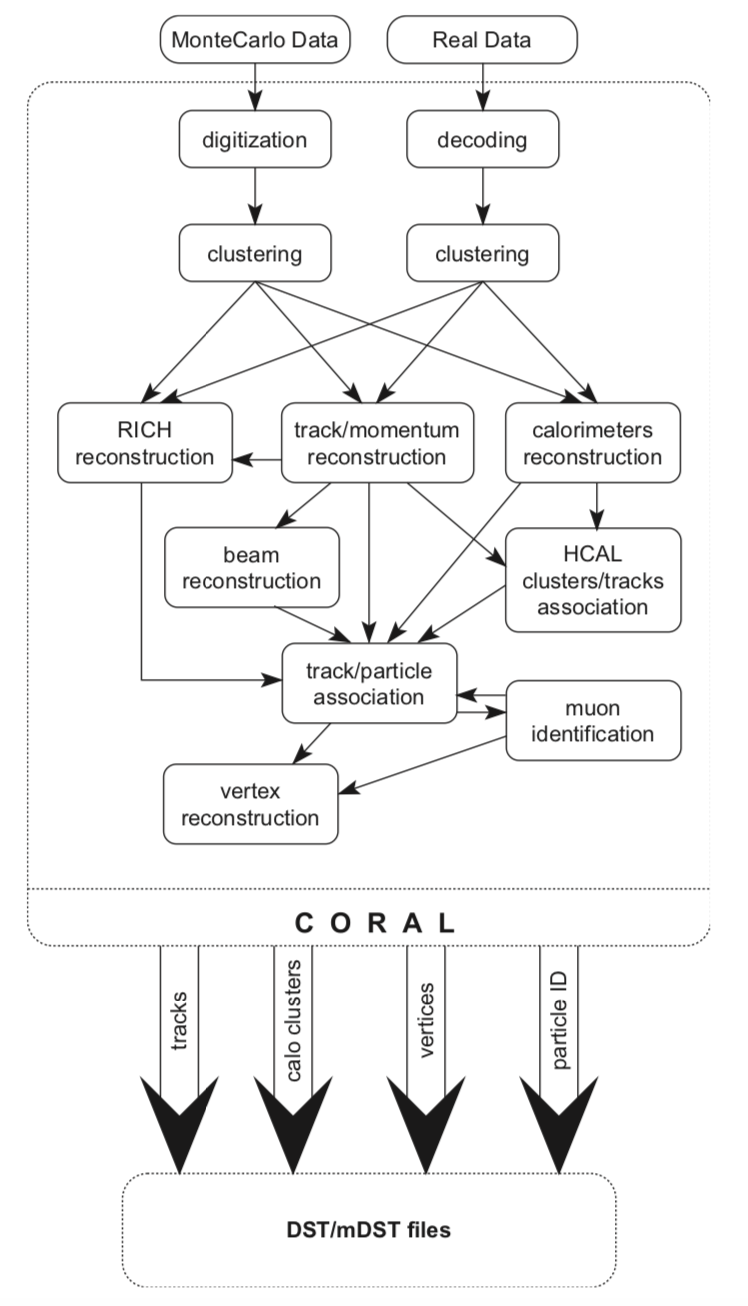
\includegraphics[scale=0.55]{./gfx/CORAL.png}
	\caption{Schematic representation of the COMPASS reconstruction software. Taken from \cite{NIM}.}
	\label{pic:CORAL}
\end{figure}
 % Chapter 3
%% Chapter 4

\chapter{RICH Detector}
\label{ch:RICH} % For referencing the chapter elsewhere, use \autoref{ch:name}

%----------------------------------------------------------------------------------------

The particle identification is an important step in the hadron multiplicity extraction. In the COMPASS spectrometer it is performed by a large Ring Imaging Cherenkov detector (RICH) capable of separating pions, kaons and protons in a wide momentum range ( $\sim$$2$ GeV/$c$ to $\sim$$55$ GeV/$c$) and an angular aperture of $0.01$-$0.4$ radians.

In this chapter the RICH detection principle is presented as well as the description of its main components: the gas and mirror system, the photon detectors, the readout electronics and the data reconstruction.

\section{Cherenkov effect}

When a charged particle is moving through a transparent medium with a speed v greater than the speed of light (v$_{light} = c/n$, $n$ being the medium refractive index), a radiation known as \textit{Cherenkov radiation} is produced by the medium.

\begin{figure}[!h]
  \centering
	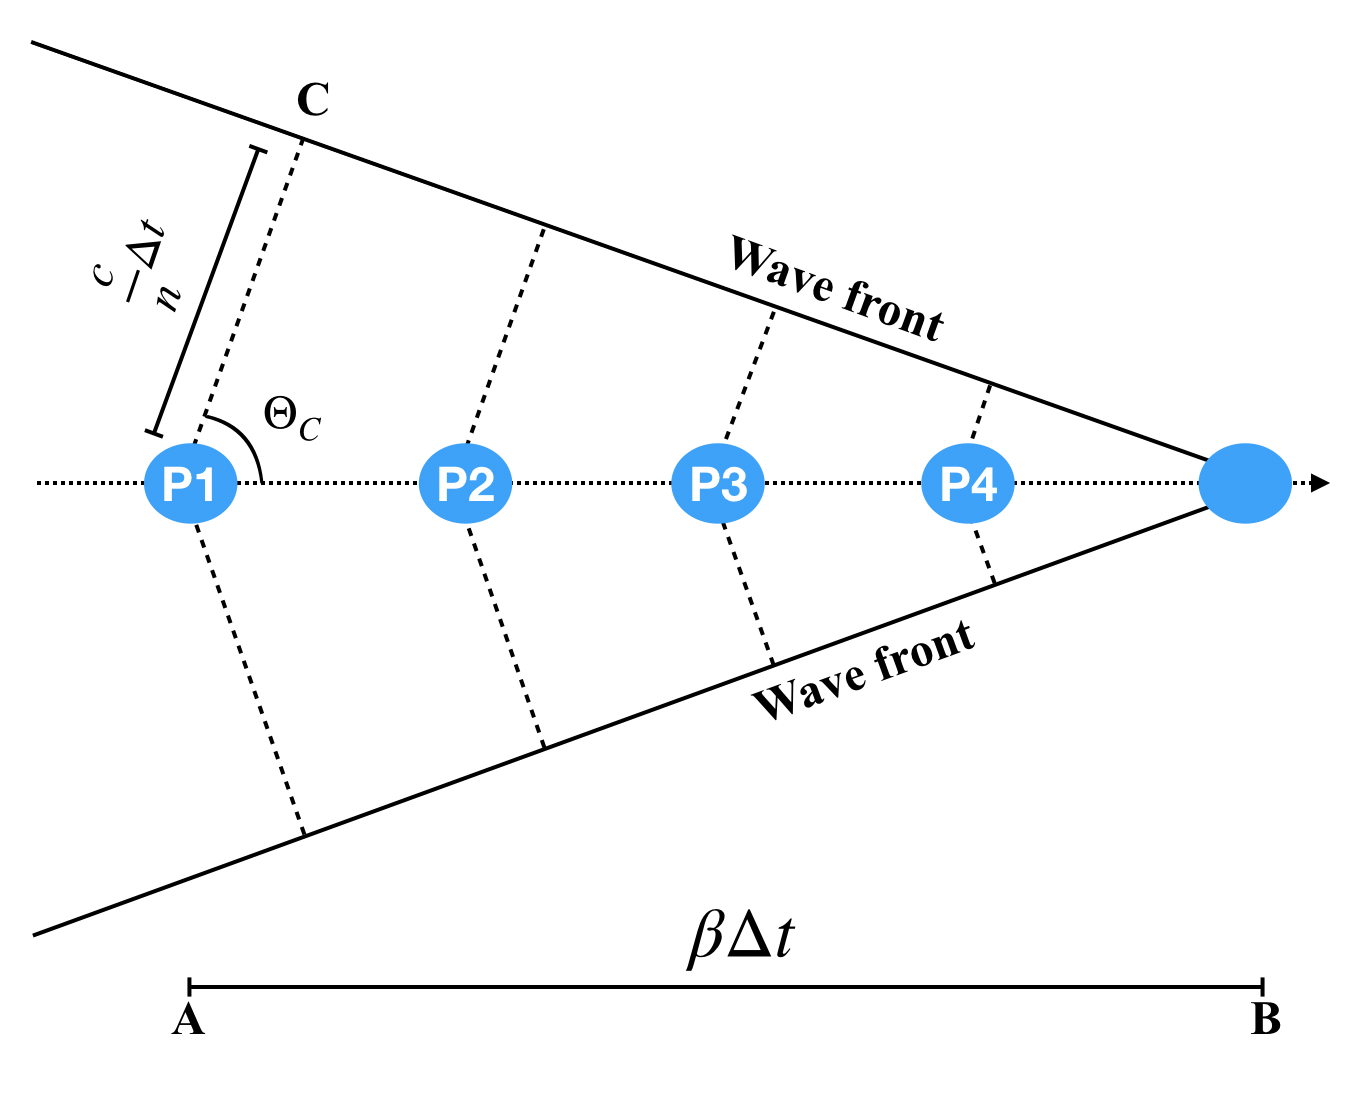
\includegraphics[scale=0.5]{./gfx/CherenkovGeom.png}
	\caption{Cherenkov radiation geometry.}
	\label{pic:CherenkovGeom}
\end{figure}

The Cherenkov radiation produced by a particle with a mass $M_h$ and momentum $p_h$ is emitted in a narrow cone around a particular angle $\Theta_C$ with respect to the particle track (Fig.~\ref{pic:CherenkovGeom}). The wavelength of these radiations goes from visible to UV.

The coherence between waves (emitted between A and B) is achieved, when the particle traverses $\overline{AB}$ at the same time as the radiation travels from A to C. The opening angle $\Theta_C$ is defined geometrically in Eq.~\ref{eq:thetaC} with $\beta$ being the particle velocity over the speed of light.
%
\begin{equation}
  cos\Theta_C = \frac{c/n \Delta t}{\beta c \Delta t} = \frac{1}{n\beta}
  \label{eq:thetaC}
\end{equation}
%
Some limit cases can be devised:
\begin{enumerate}
  \item Threshold limit: if $\beta \leq 1/n$ no Cherenkov radiation will be emitted.
  \item Maximum emission angle: $cos \Theta_C = \frac{1}{n}$ is reached for ultra-relativistic particles ($\beta = 1$).
\end{enumerate}

In order to perform particle identification with a RICH detector, two variables have to be measured: $\Theta_C$ and $p_h$. The angle can be measured detecting the emitted photons. Different techniques can be used to collect and transport the produced photons to the location of the light detectors. The resulting image in the detector plane is a ring, only for specific techniques, if one does a proper optical image. In such a case the ring has a radius proportional to $\Theta_C$. $p_h$ is measured independently by the spectrometer. The particle mass can thus be calculated by:
%
\begin{equation}
  M_h = p_h \sqrt{n^2 cos^2 \Theta_C -1}
\end{equation}

%------------------------------------------------

\section{The COMPASS RICH detector}

The COMPASS RICH detector is designed to distinguish between pions, kaons and protons at high intensities. The momentum range covers the pion Cherenkov threshold ($\sim$ $2.67$ GeV/c) to $\sim$ $55$ GeV/c.

The RICH is a large size detector ($\sim$ $3$ x $5$ x $6$ m$^3$, see Fig.~\ref{pic:RICHview}) filled with a gaseous radiator. Two spherical mirror systems reflect the photons into an array of photon detectors sensitive to a large wavelength range, from visible to far UV, placed outside the spectrometer acceptance, one above and one below the beam line. The goal is to count as many photons as possible with a good spacial resolution. The whole structure of the detector vessel is built mainly in thin aluminium in order to minimize the material budget.

Until $2004$, MultiWire Proportional Chambers (MWPC) equipped with solid-state CsI photo-cathodes were used to detect Cherenkov photons. The gains of the MWPC operation was limited. The first stage of the electronic readout was characterized by a long integration time, which was a limiting factor in the COMPASS environment as there is a high-rate uncorrelated background due to the large muon halo beam. Moreover, the long base-line restoration time generated a non-negligible dead time. To overcome these limitations, the central region that covers $25$\% of the photo-detection surface was replaced with MultiAnode PhotoMultiplier Tubes (MAPMT). They are intrisically fast and have better time resolutions.

\begin{figure}[!h]
  \centering
	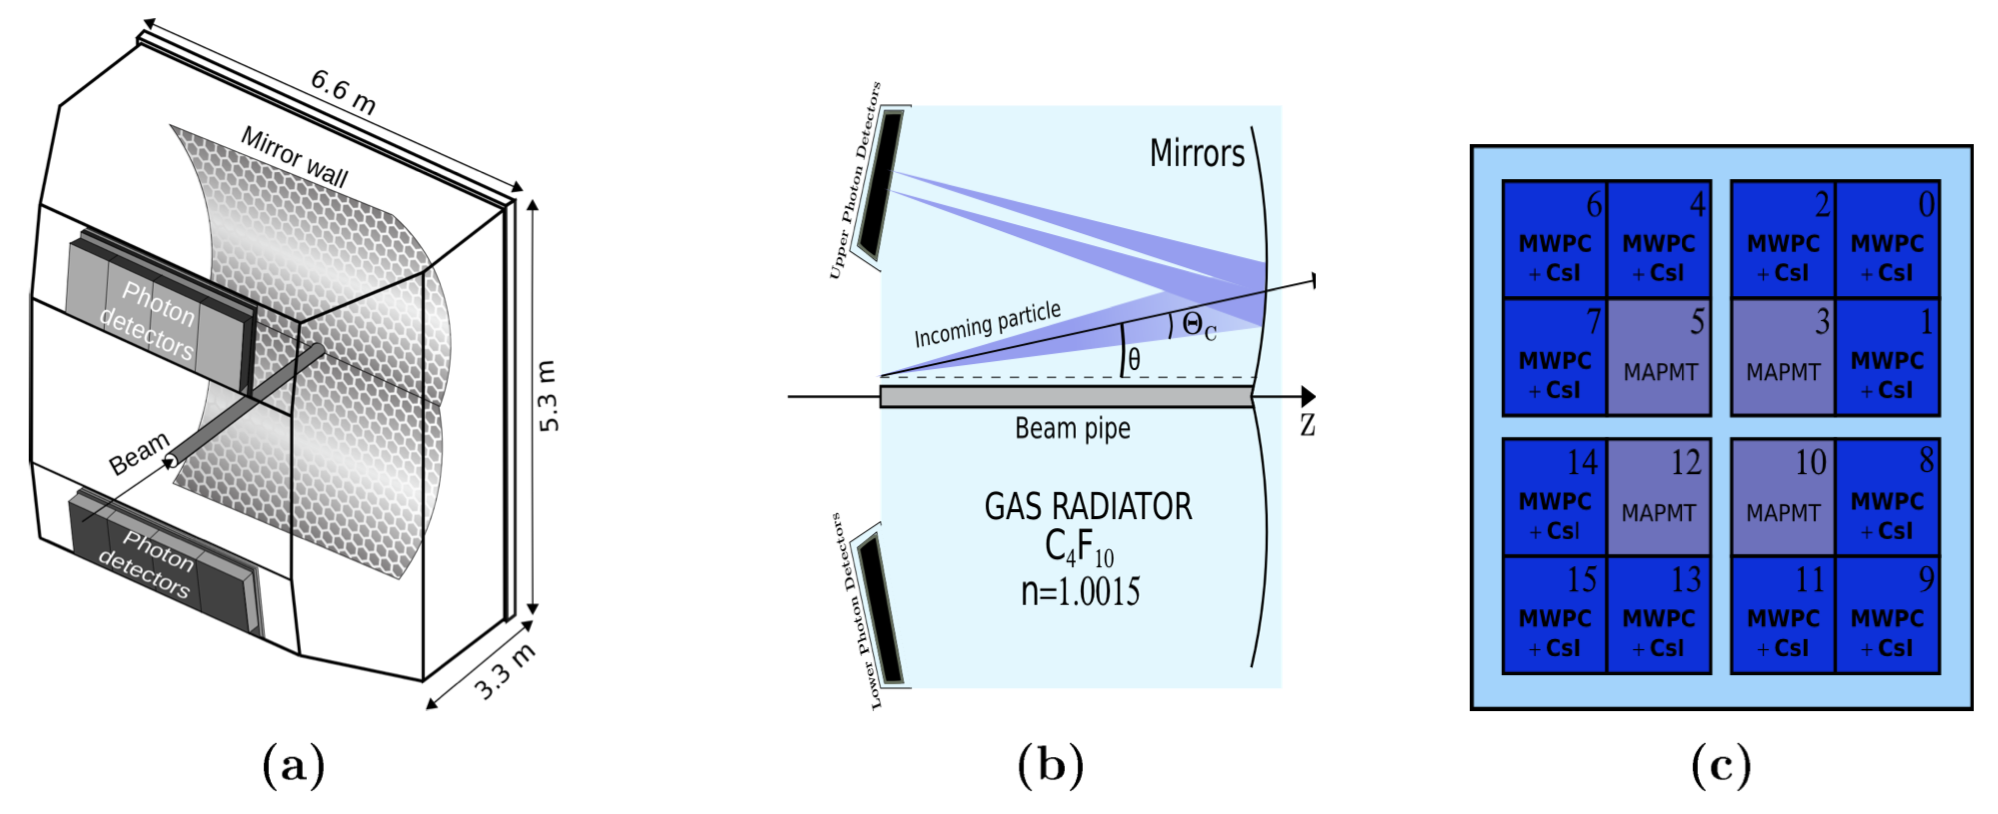
\includegraphics[scale=0.4]{./gfx/RICHview.png}
	\caption{(a) Artistic view of the COMPASS RICH detector. (b) Basic functioning of the RICH detector. (c) Photon detector disposition (not to scale).}
	\label{pic:RICHview}
\end{figure}

\subsection{Gas System}

One of the principal elements of a RICH detector is the radiator. At COMPASS it is perfluorobutane (C$_4$F$_{10}$). It has a refractive index of n $\approx$ $1.0015$ and a low chromaticity\footnote{Dependence of the refractive index of a dielectric medium on the photon wavelength \cite{Dispersion}} ($dn/dE_{\gamma}$ of about $5 \cdot 10^{-5}$~eV$^{-1}$). These characteristics allow the particle identification (PID) to be performed in the aforementioned wide momentum range.

The propagation of the Cherenkov photons in the vessel can be affected by the presence of water vapor and oxygen (high UV light absorption cross section). In order to remove these impurities, the gas is constantly circulating and filtered at a constant pressure (1 mbar higher than the atmospheric pressure) in a dedicated gas system \cite{RICHGas}. The overpressure of the vessel is needed to prevent air contamination and to avoid mechanical stress to the detector, given its large size. Other circulation system (known as \textit{fast circulation} system) allows a reshuffling of the gas inside the vessel: as perfluorobutane has a density of $11.21$ kg/m$^3$ it avoids stratification that may cause a gradient in the value of the refractive index from top to bottom.

In order to absorb the photon emitted by the muon beam, a $10$ cm diameter pipe filled with helium is positioned inside the vessel along the beam.

\subsection{Mirror System}

The RICH optical system covers an area of $\sim$ $21$ m$^2$ and consists of two spherical surfaces, each one containing $58$ spherical mirrors of different shapes ($34$ hexagons and $24$ pentagons). The mirror pattern is shown in Fig.~\ref{pic:RICHmirrors}. All the mirrors have a reflectance above $80$\% in the UV region.

The mirror system has a radius of curvature of $6.6$ m. The photon image is focused outside the spectrometer acceptance where the photon detectors are located. As the radii of the curvature have a scatter of $1$\% (R = $6600\pm66$ mm), the reflected image is slightly blurred. This effect is more pronounced for particles at large angles \cite{RICHMirror}: this aberration contributes to the dispersion of the photon angle with respect to the angle of emission, which affects the detection resolution \cite{RICHPID}.

\begin{figure}[!h]
  \centering
	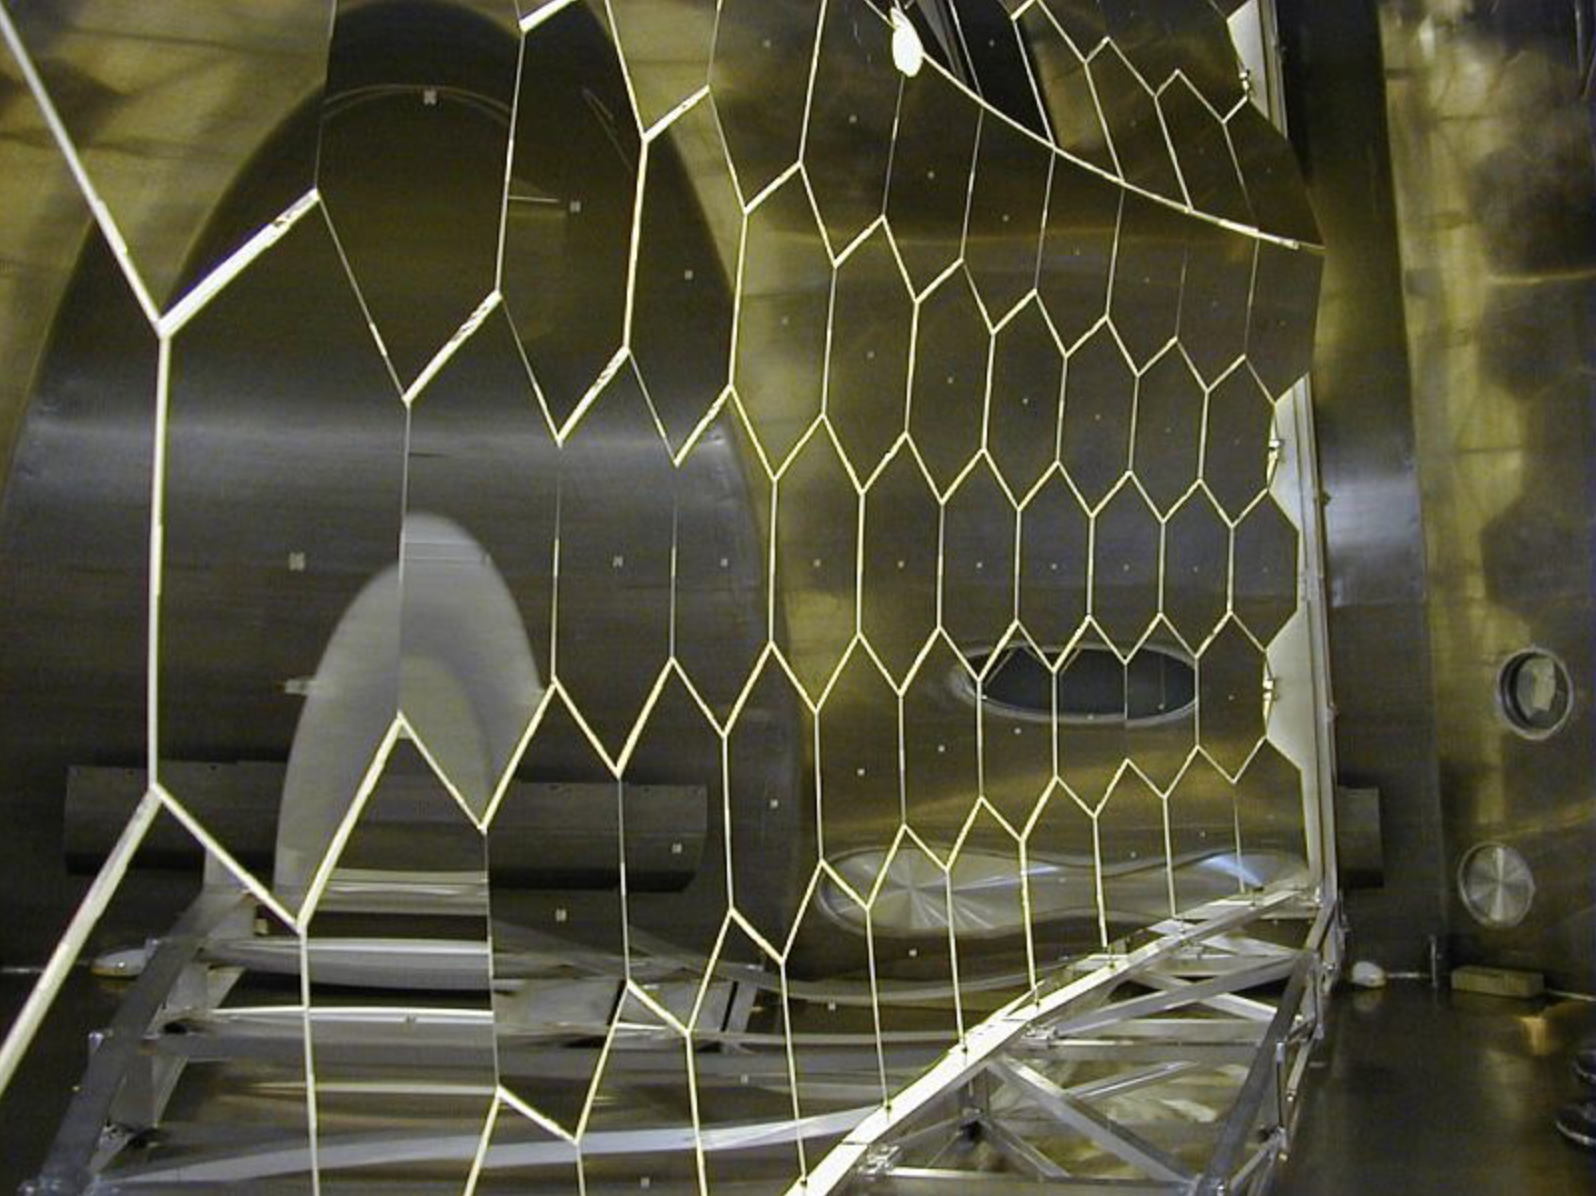
\includegraphics[scale=0.4]{./gfx/RICHmirrors.png}
	\caption{COMPASS RICH detector optical system.}
	\label{pic:RICHmirrors}
\end{figure}

\subsection{Photon Detectors}

The photon detector array consists of two symmetric parts with respect to the beam line, each one is composed of $8$ modules located at the mirror focal plane. The modules in the external regions are MultiWire Proportional Chambers (MWPC) equipped with solid state CsI photo-cathodes \cite{RICHLimits}. The central area is composed by MultiAnode Photomultiplier Tubes (MAPMT) \cite{RICHUpgrade} coupled to individual telescopes of fused silica lenses. The use of two different detector types employing different different photon converters results in the detection of photons in two wavelength regions: < $200$ nm for MWPCs and $\sim$ $200$ - $650$ nm for MAPMT. The low momentum particles are mainly detected by the outer part (MWPC), while the high momentum ones are detected by the central part (MAPMT). Only the central part is used in the following analysis.

The spherical mirrors will focus all the photons emitted parallel in the same point. Thus the Cherenkov light cone of our particle will result in a ring at the detector plane. The distribution of photons in the detectors for a physics event is shown in Fig.~\ref{pic:RICHEvent}.

\begin{figure}[!h]
  \centering
	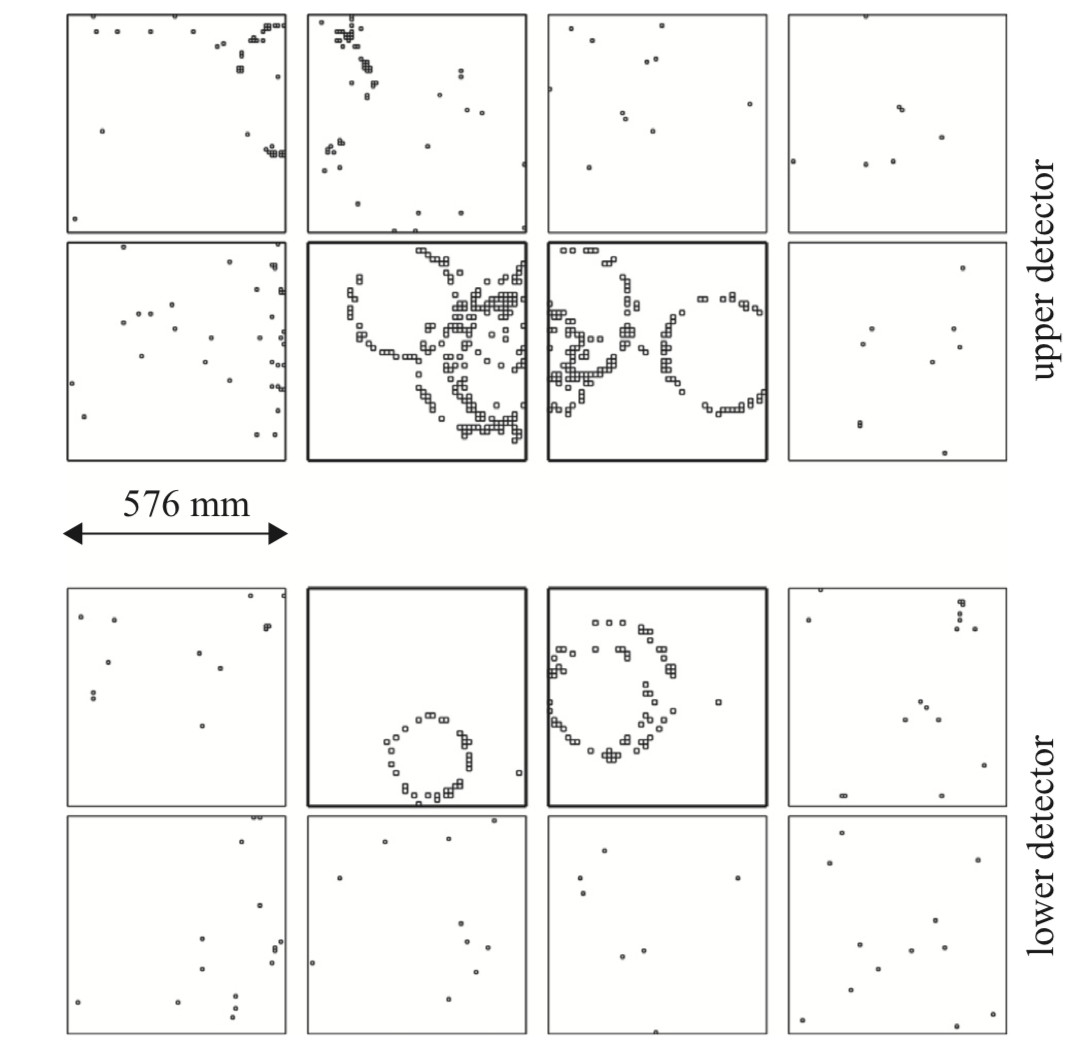
\includegraphics[scale=0.5]{./gfx/RICHEvent.png}
	\caption{An event from the online event display of COMPASS RICHONE. The $16$ squares represent the detectors areas ; the four central ones are equipped with MAPMTs. the small squares represent the hits with signal amplitudes larger than a threshold, individually set for each channel. Figure taken from \cite{NIM2015}}
	\label{pic:RICHEvent}
\end{figure}

\subsection{RICH Infos Reconstruction}

RICHONE is a package contained in the CORAL software, which is in charge of RICH information reconstruction. The reconstruction is divided in several parts, the first being decoding the data and clustering. Then the reconstruction of the Cherenkov angle for each individual photon is done. It is possible to perform a ring reconstruction which is used for studies on the apparatus. The particle identification (PID) is based on a maximum likelihood calculation. The PID will be explained more thouroughly afterwards.

\subsubsection*{Decoding and clustering}

There are two different types of photon detectors and they have different decoding systems and clustering algorithms. For the MWPCs, if more than one channel fires, a clustering is done. When the pad with the highest pulse height is found, all the adjacent pads with a smaller signal are included in the cluster \cite{RICHPID}. The mean position of each active pad is evaluated in the cluster, weighting the signal with their maximum pulse height, to determine the center of gravity of the cluster. For the MAPMT, decoding the signal is enough to read the time information coming from the PMT that was hit. As the probability of having correlated hits in adjacent area is negligible, the MAPMT data does not need clustering \cite{RICHElec}.

The cluster or hit position is used to determine the trajectory of the photon. In addition, the time information coming from the MAPMT is used to reject out-of-time photons while the amplitude information from the MWPC serves to reduce the background both from out-of-time photons and from electronic noise \cite{RICHPID}.

\subsubsection*{Cherenkov angle and ring reconstruction}

The ring reconstruction begins with the selection of a particle tracks. Then one looks for the photons around this track. The trajectory of each Cherenkov photon is calculated with respect to the plane containing the particle track and its virtual reflection in the mirror in order to reconstruct $\Theta_C$ \cite{RICHTheory}. All the photons emitted by one particle are expected to have the same angle $\Theta_C$ and to be uniformly distributed in $\phi$. The photons emitted by other particles or from background have on the contrary a flat $\Theta_C$ distribution. The emitted photon with the same ($\Theta_C$,$\phi$) pair are reflected on the same location at the focal surface (neglecting any spherical aberration), resulting in a ring image of the photon detector. Since the emission point of the photon along the particle trajectory is not known, the middle point between the detector and the mirror is taken. A good determination of the track trajectory parameters and the momentum of the particle are mandatory in order to extract $\Theta_C$ with good precision.

To characterize the RICH, determining its angular resolution for instance, the ring reconstruction of the emitted photons is needed. The ring reconstruction is based on the search of a peak in the $\Theta_C$ distribution. Small intervals of $\pm$3$\sigma$ ($\sigma$ being the single photon resolution, $\sigma_{MAPMT}$ = $2.0$ mrad and $\sigma_{MWPC}$ = $2.5$ mrad) on an overall range of $0$ to $70$ mrad are considered. The interval with the maximum number of entries is used to define the ring. This procedure associates a ring to each track and in order to reject tracks with only background photons a minimal amount of photons per ring is required (four photons for the MAPMT part) \cite{RICHPID}. The resolution of the Cherenkov angle measurement provided by each single photon as a function of the particle momentum is illustrated in Fig.~\ref{pic:RICHRez}.

\begin{figure}[!h]
  \centering
	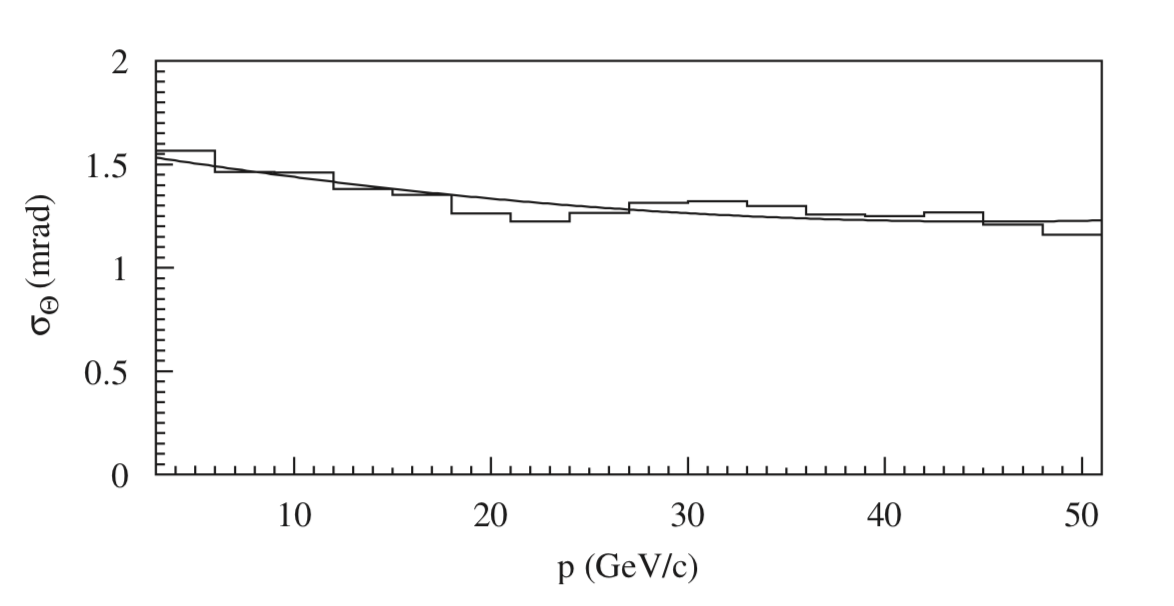
\includegraphics[scale=0.5]{./gfx/RICHRez.png}
	\caption{Resolution of the Cherenkov angle for the reconstructed ring images, provided by each single photon, versus the particle momentum for a sample of identified pions. Figure taken from \cite{NIM}.}
	\label{pic:RICHRez}
\end{figure}

The measured values of $\theta_C$ as a function of $p_h$ for the RICH detector are shown in Fig.~\ref{pic:RICH}. In the low momentum region, the RICH detector is only sensitive to electrons, muons and pions. The bands corresponding to kaons and protons start to be visible respectively at $p_h \approx$ $9.45$ GeV/c and $p_h \approx$ $17.95$ GeV/c. For high momentum values above $40$ GeV/c, saturation of the Cherenkov angle is observed or pions and kaons. The final particle identification is performed using likelihood methods and is described in the following chapter.

\begin{figure}[!h]
  \centering
	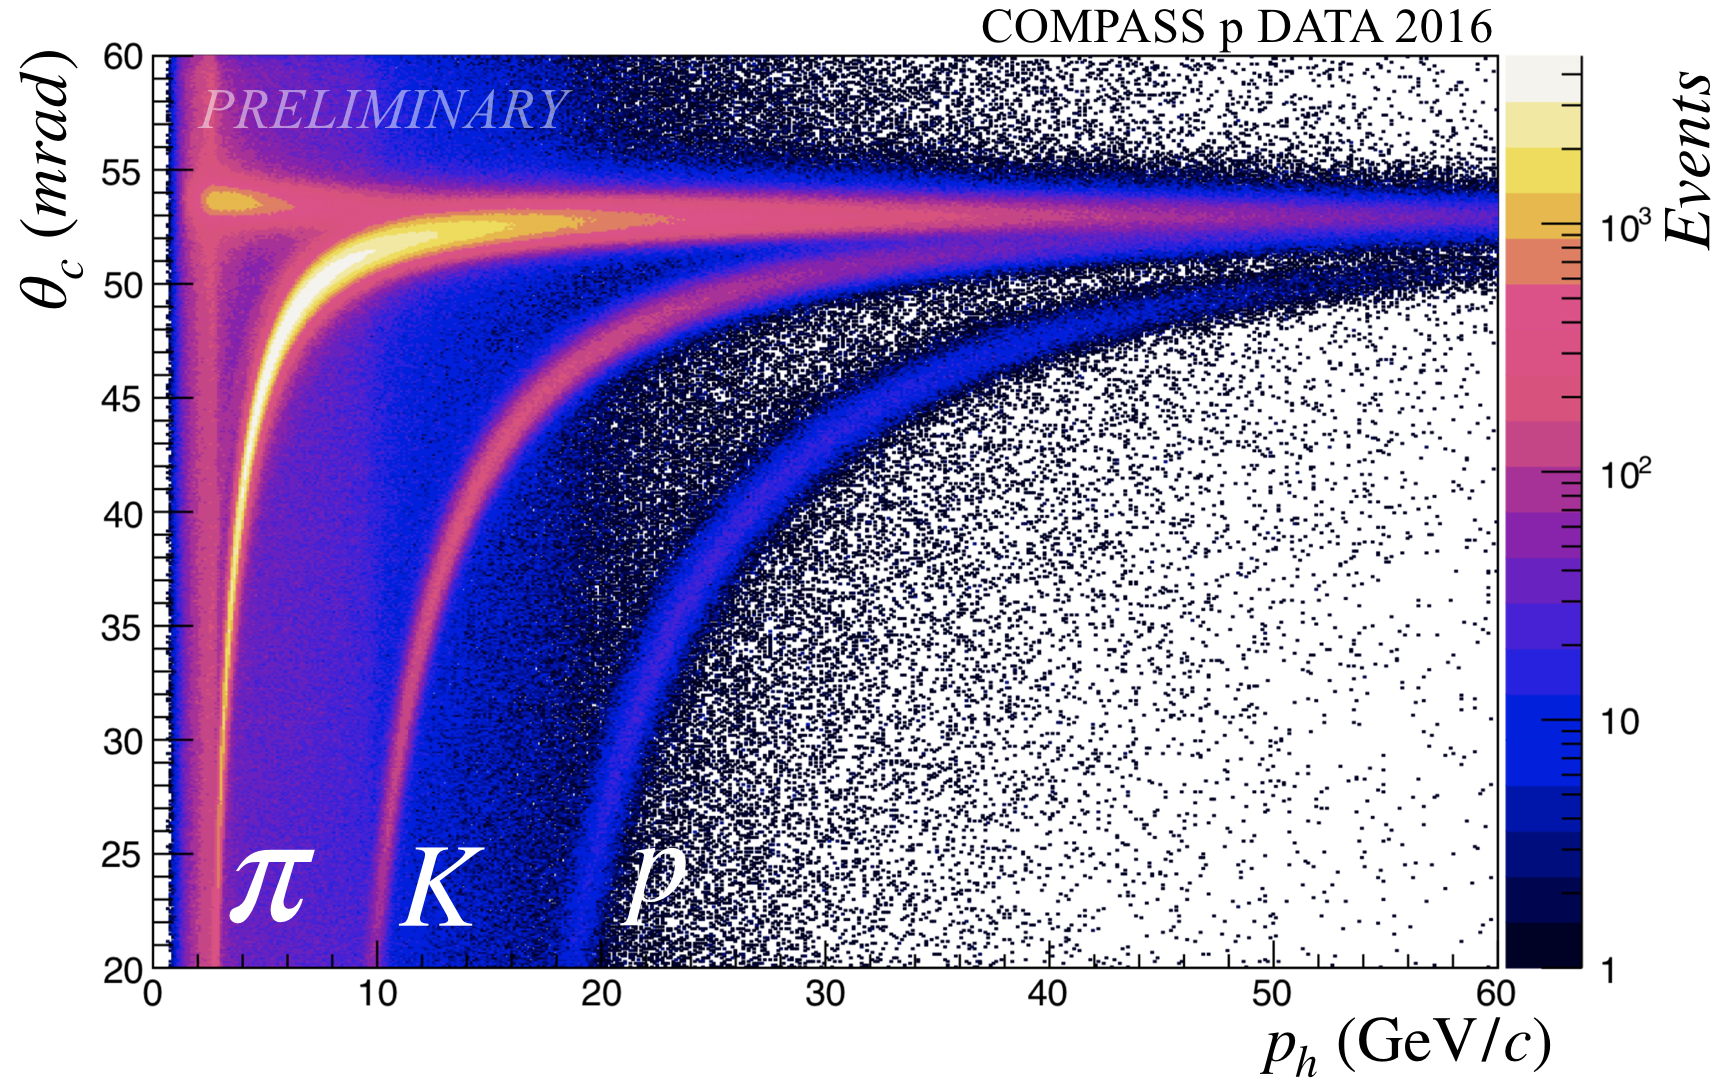
\includegraphics[scale=0.45]{./gfx/RICH.png}
	\caption{Measured Cherenkov angle $\Theta_C$ as a function of $p_h$. $\pi$ threshold is about $2.67$ GeV/$c$, $K$ threshold about $9.45$ GeV/$c$ and $p$ threshold about $17.95$ GeV/$c$, respectively.}
	\label{pic:RICH}
\end{figure}
 % Chapter 4 - empty template

\cleardoublepage % Empty page before the start of the next part

%----------------------------------------------------------------------------------------
%	THESIS CONTENT - APPENDICES
%----------------------------------------------------------------------------------------

\appendix

\part{Appendix} % New part of the thesis for the appendix

% Appendix A

\chapter{Systematic studies follow-up}

%----------------------------------------------------------------------------------------

\section{Systematic uncertainty associated with the RICH}

\begin{figure}[!p]
  \centering
	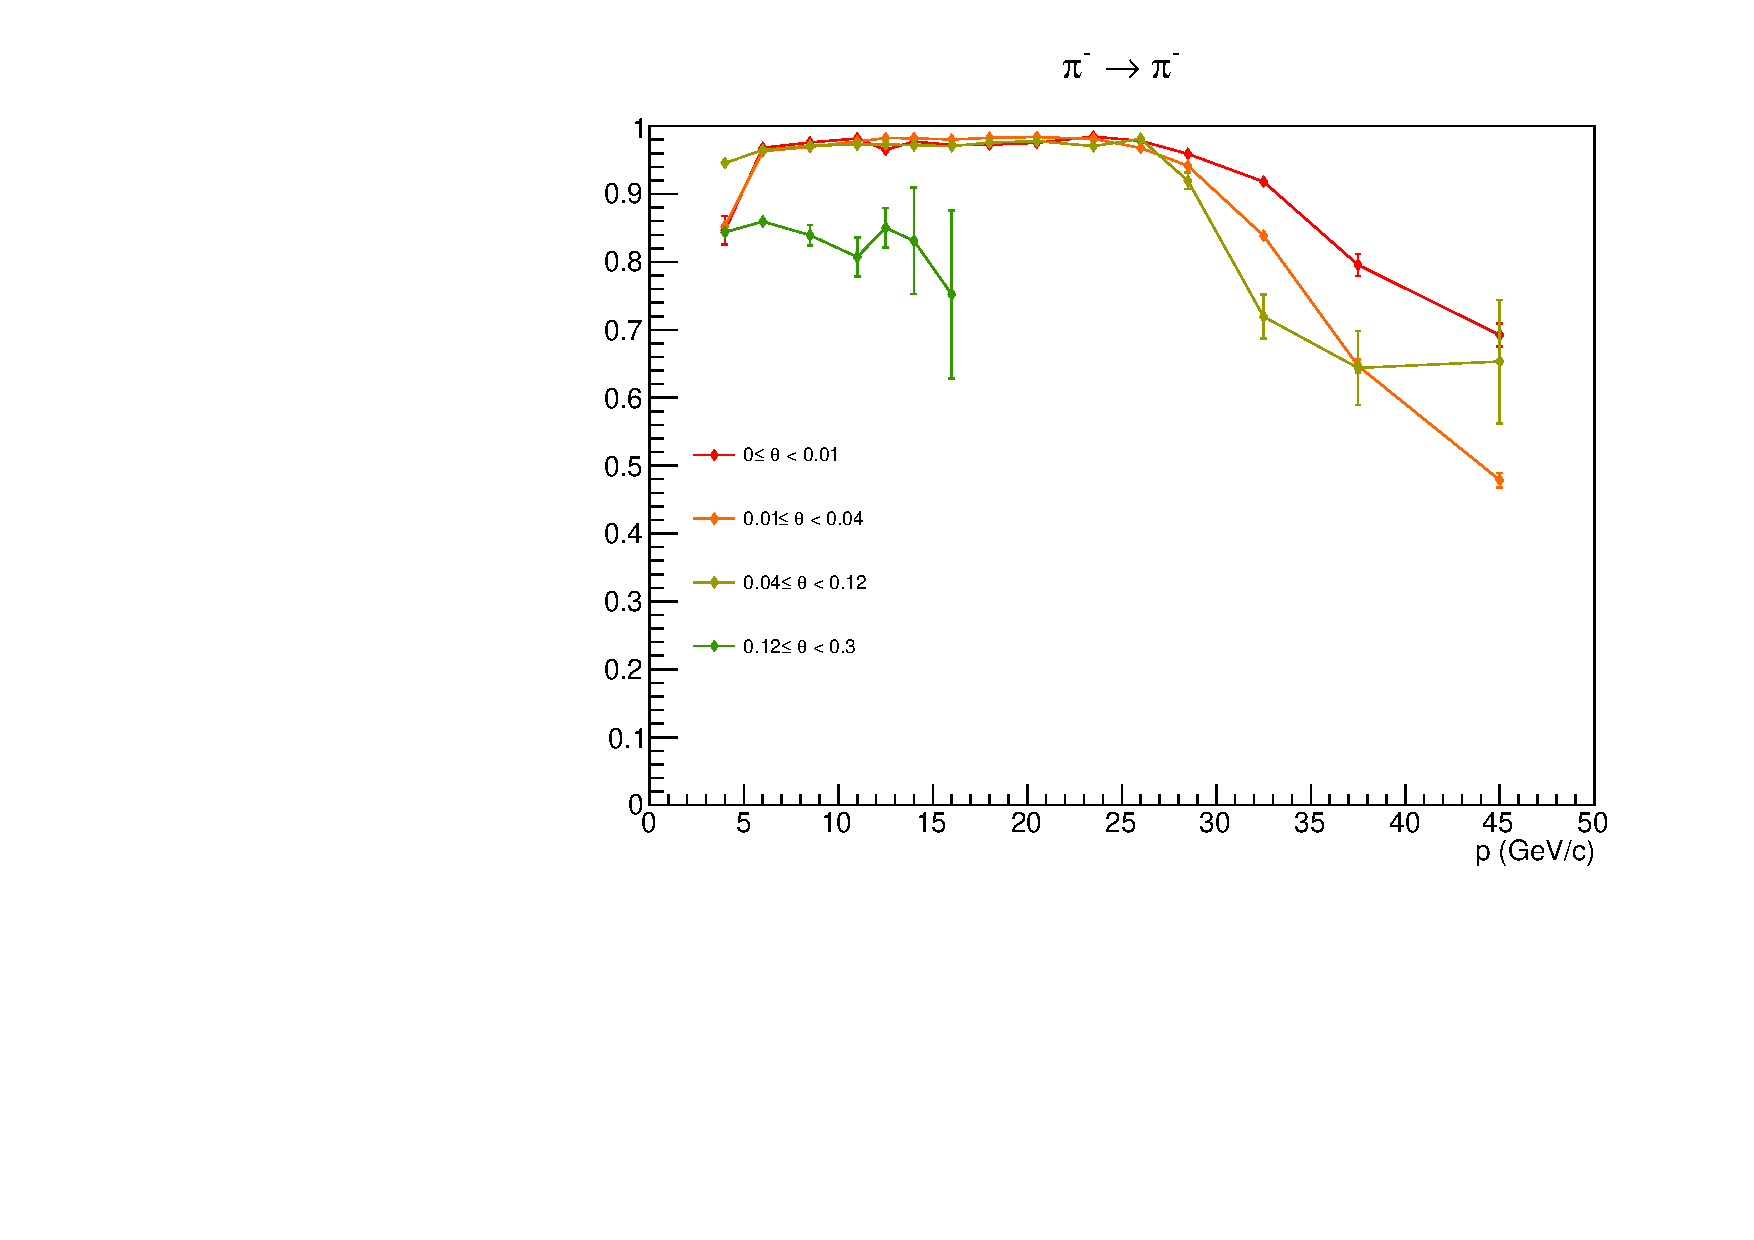
\includegraphics[scale=0.38]{./gfx/pim_pi.pdf}
  \includegraphics[scale=0.38]{./gfx/pim_K.pdf}
  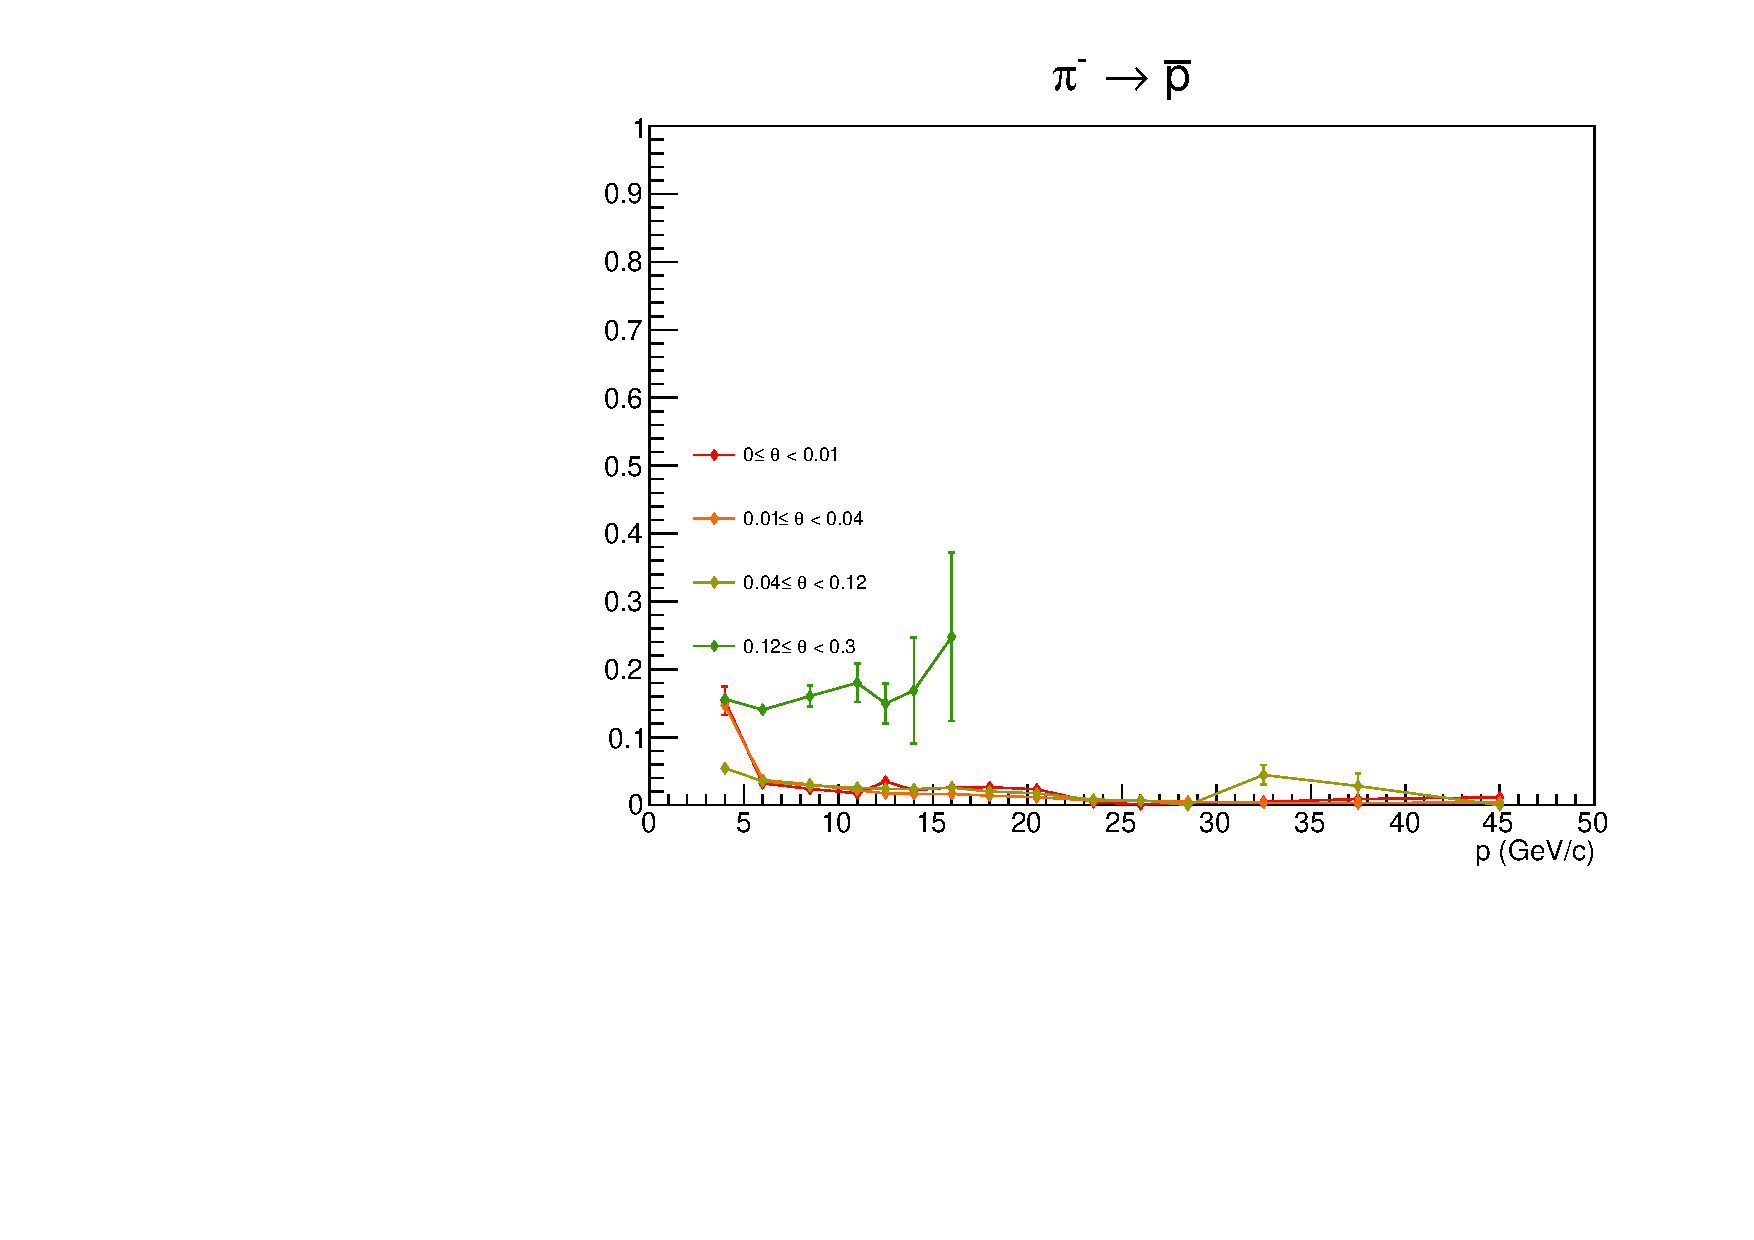
\includegraphics[scale=0.38]{./gfx/pim_p.pdf}
  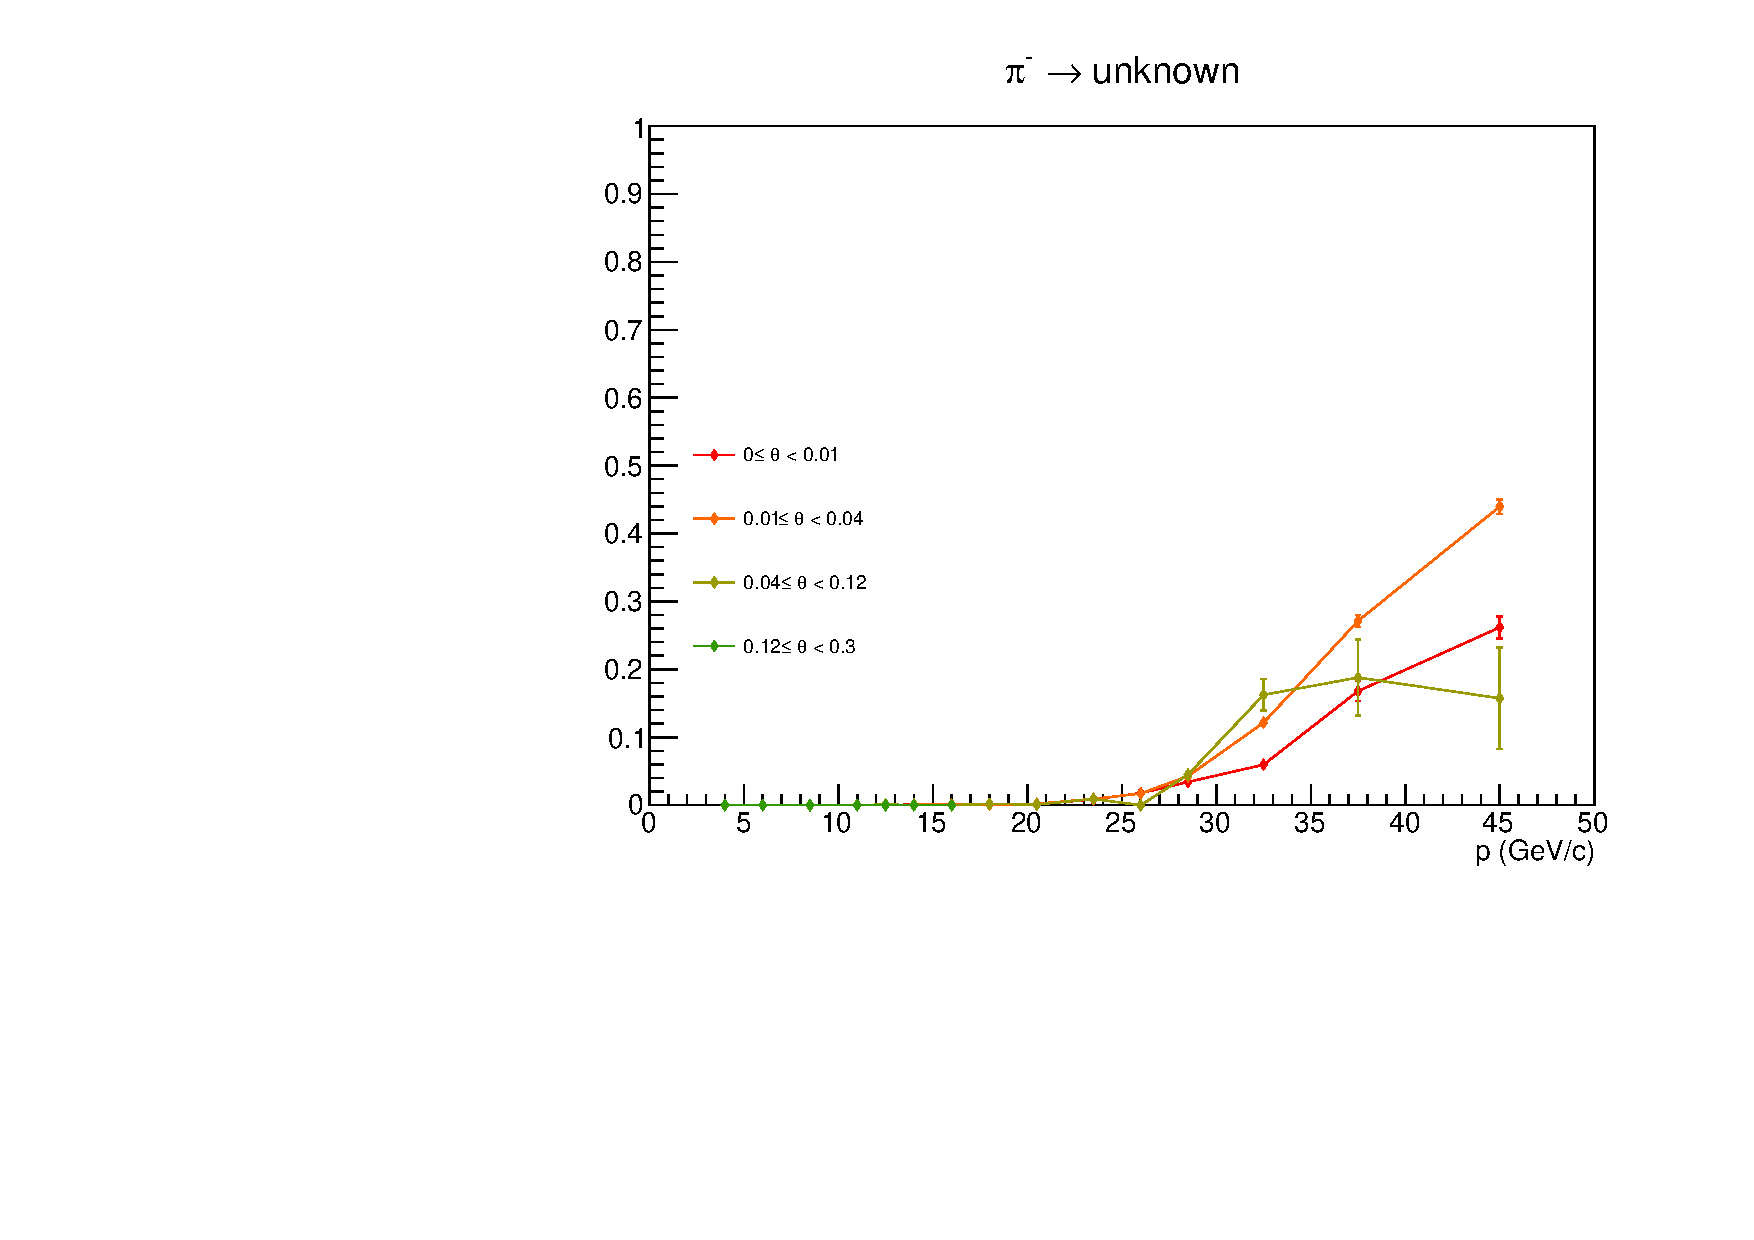
\includegraphics[scale=0.38]{./gfx/pim_u.pdf}
	\caption{Identification probabilities $\epsilon(p \rightarrow j)$ for $\pi^-$.}
	\label{pic:Effpim}
\end{figure}


\begin{figure}[!p]
  \centering
	\includegraphics[scale=0.38]{./gfx/Km_pi.pdf}
  \includegraphics[scale=0.38]{./gfx/Km_K.pdf}
  \includegraphics[scale=0.38]{./gfx/Km_p.pdf}
  \includegraphics[scale=0.38]{./gfx/Km_u.pdf}
	\caption{Identification probabilities $\epsilon(p \rightarrow j)$ for $K^-$.}
	\label{pic:Effkm}
\end{figure}

\begin{figure}[!p]
  \centering
	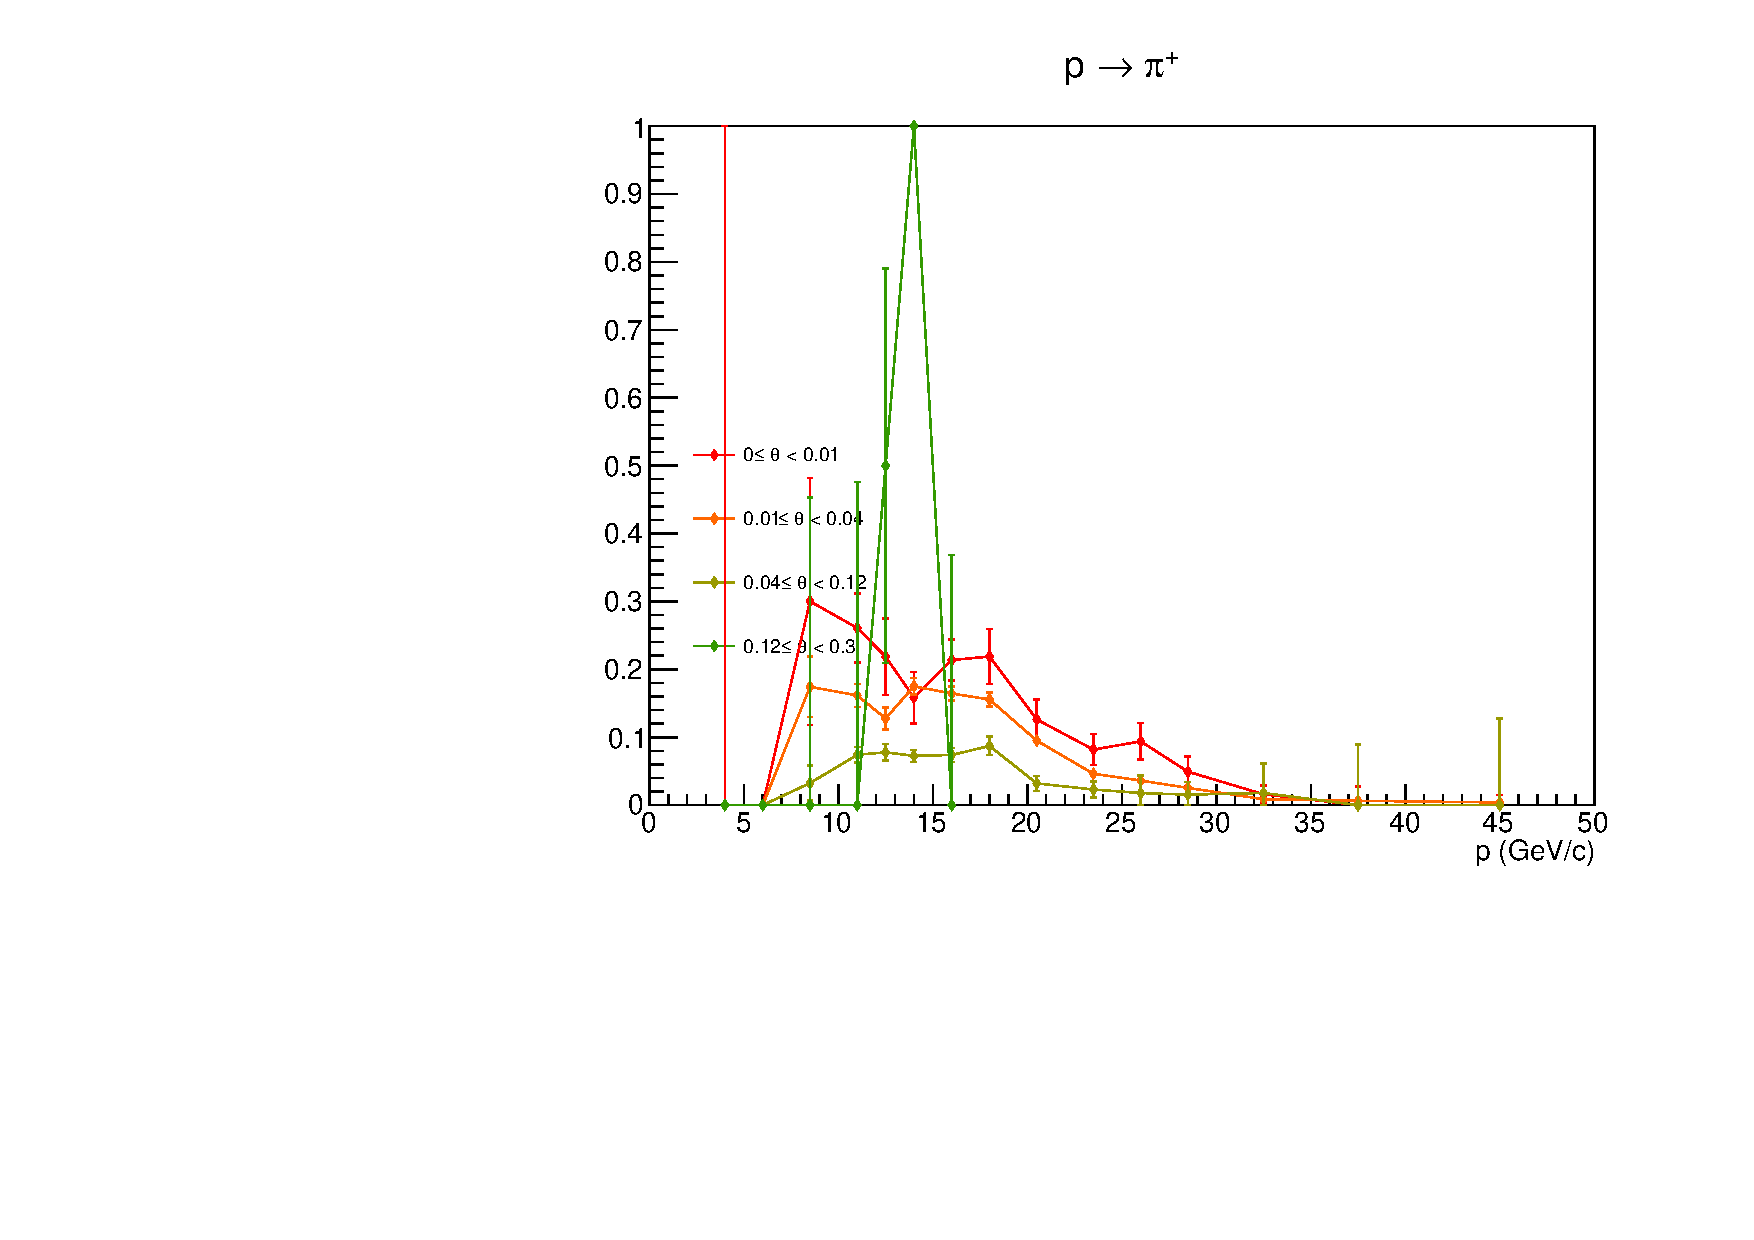
\includegraphics[scale=0.38]{./gfx/pp_pi.pdf}
  \includegraphics[scale=0.38]{./gfx/pp_K.pdf}
  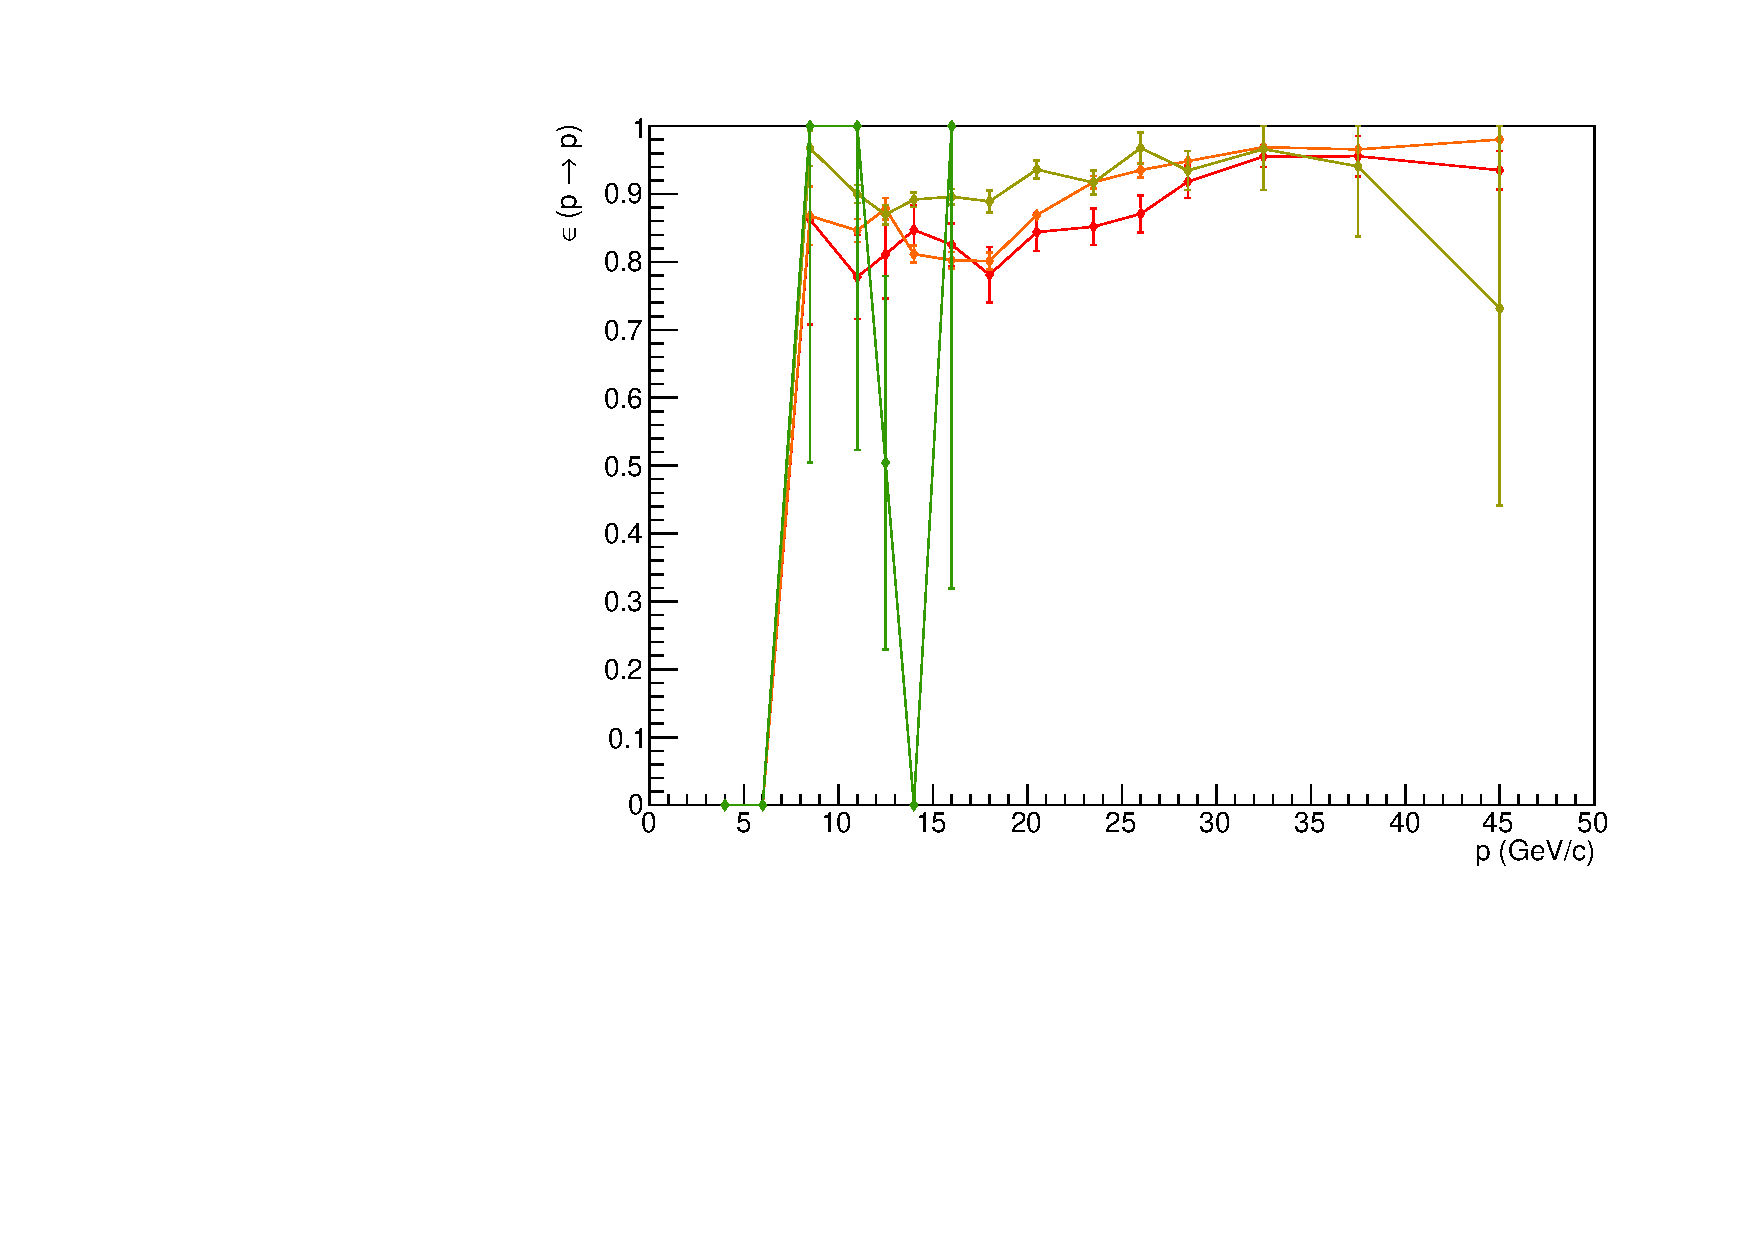
\includegraphics[scale=0.38]{./gfx/pp_p.pdf}
  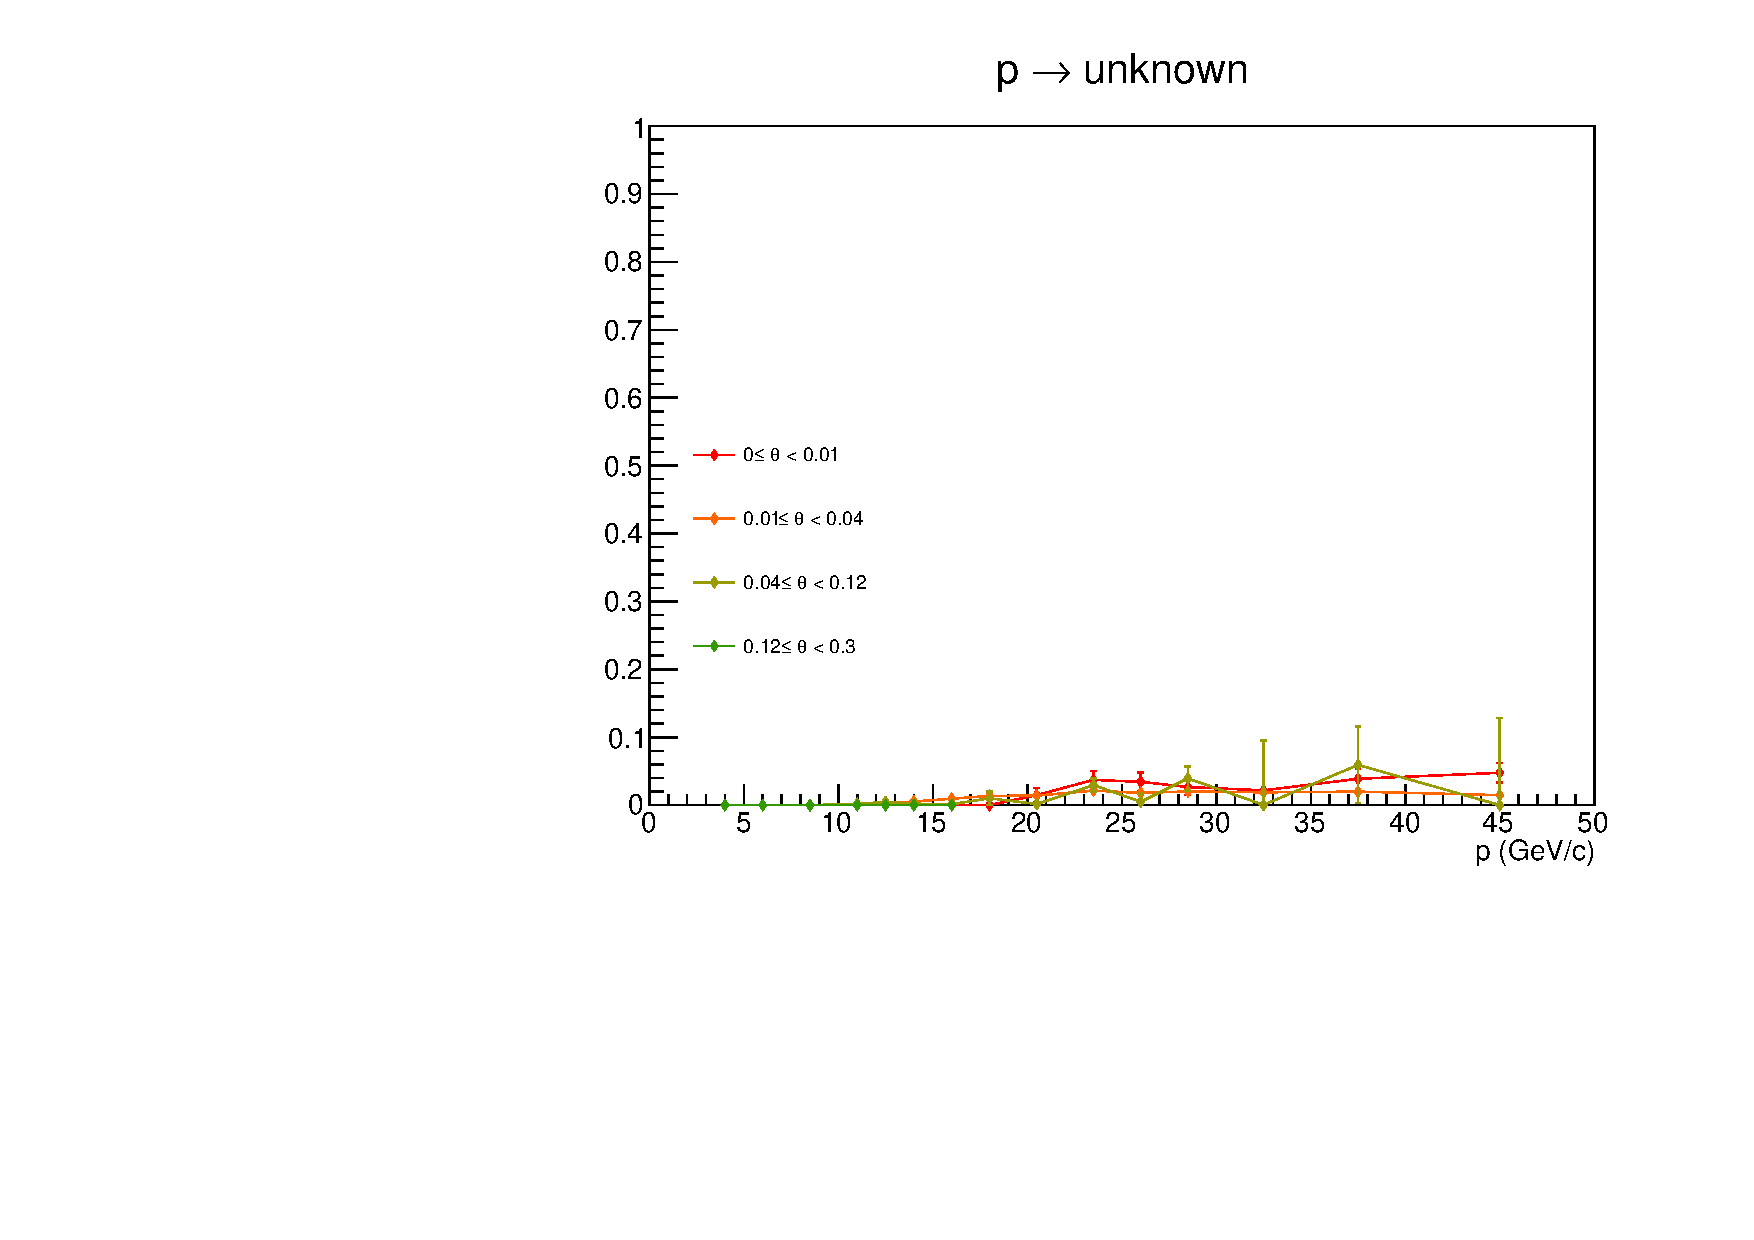
\includegraphics[scale=0.38]{./gfx/pp_u.pdf}
	\caption{Identification probabilities $\epsilon(p \rightarrow j)$ for $p$.}
	\label{pic:Effpp}
\end{figure}

\begin{figure}[!p]
  \centering
	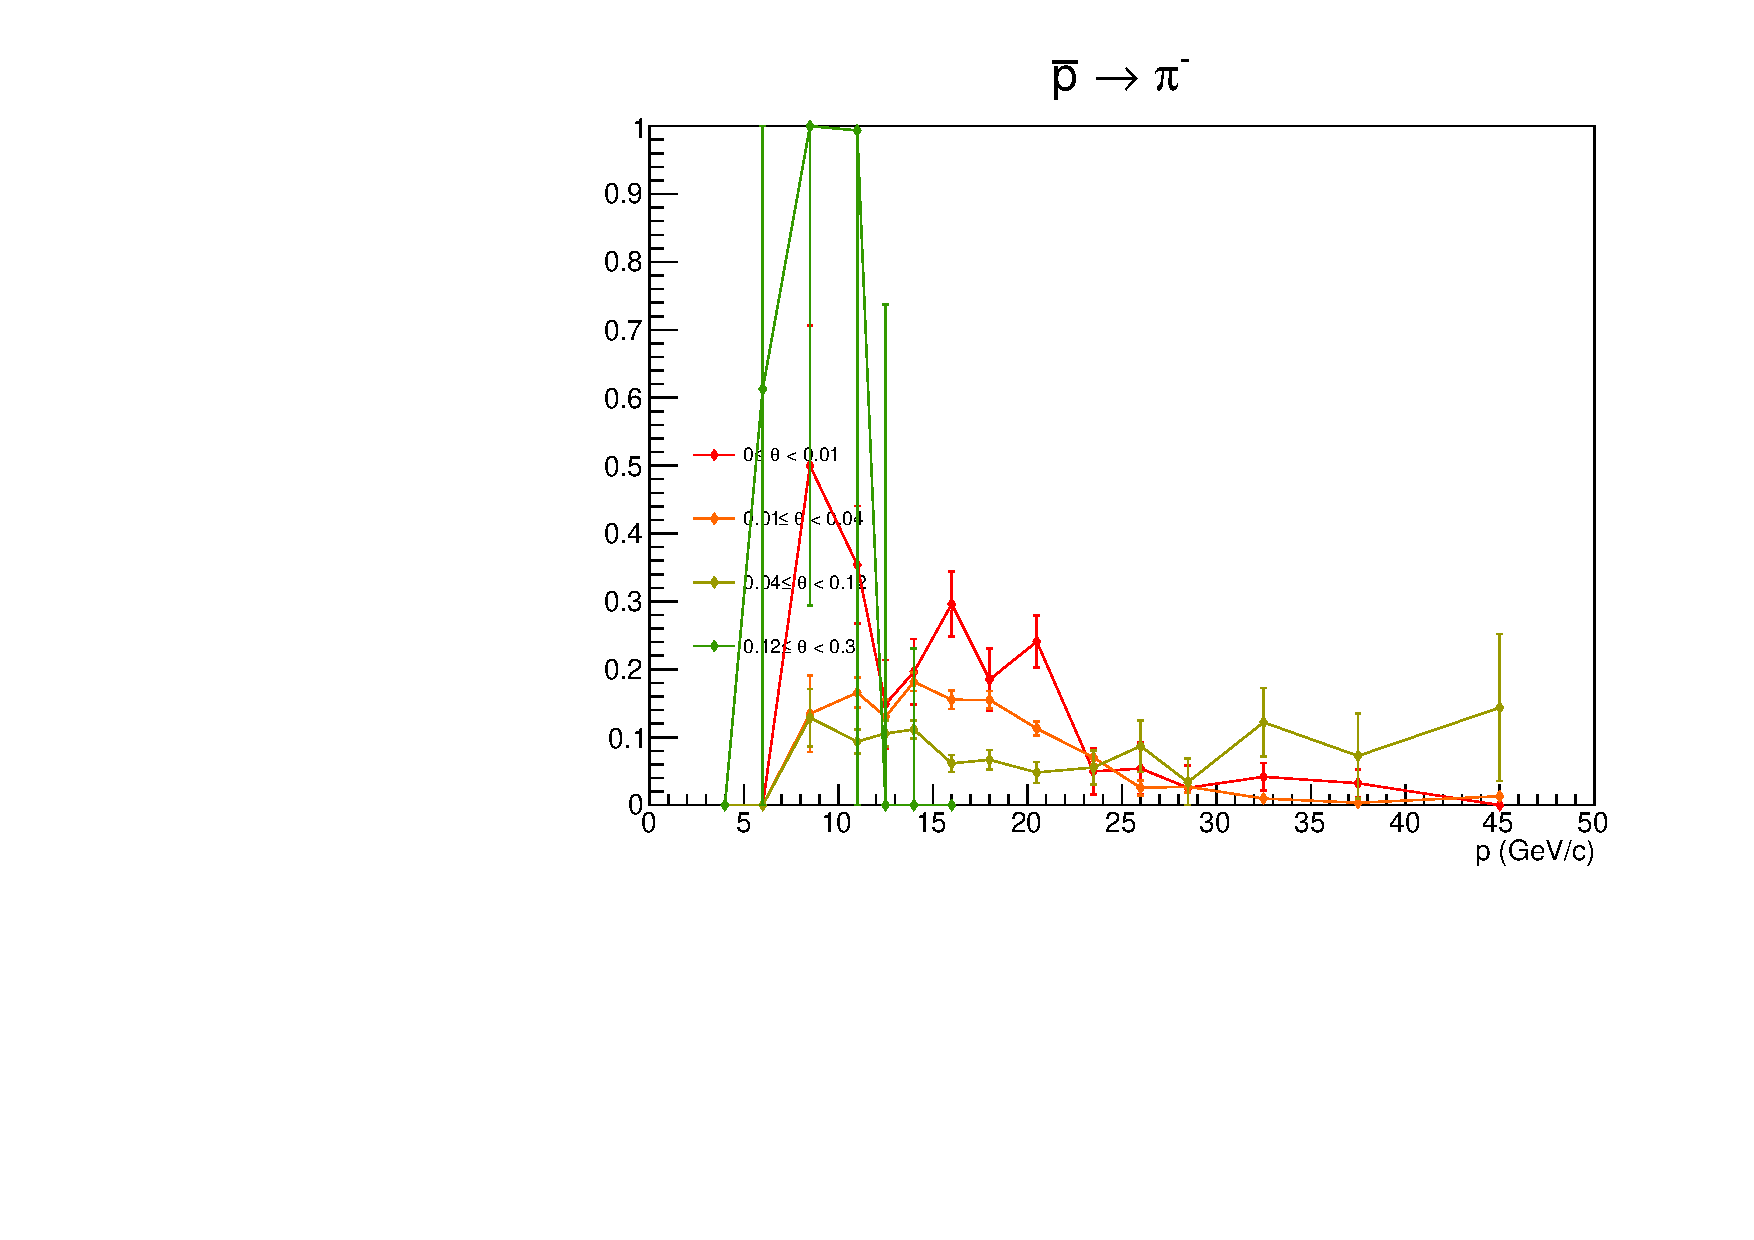
\includegraphics[scale=0.38]{./gfx/pm_pi.pdf}
  \includegraphics[scale=0.38]{./gfx/pm_K.pdf}
  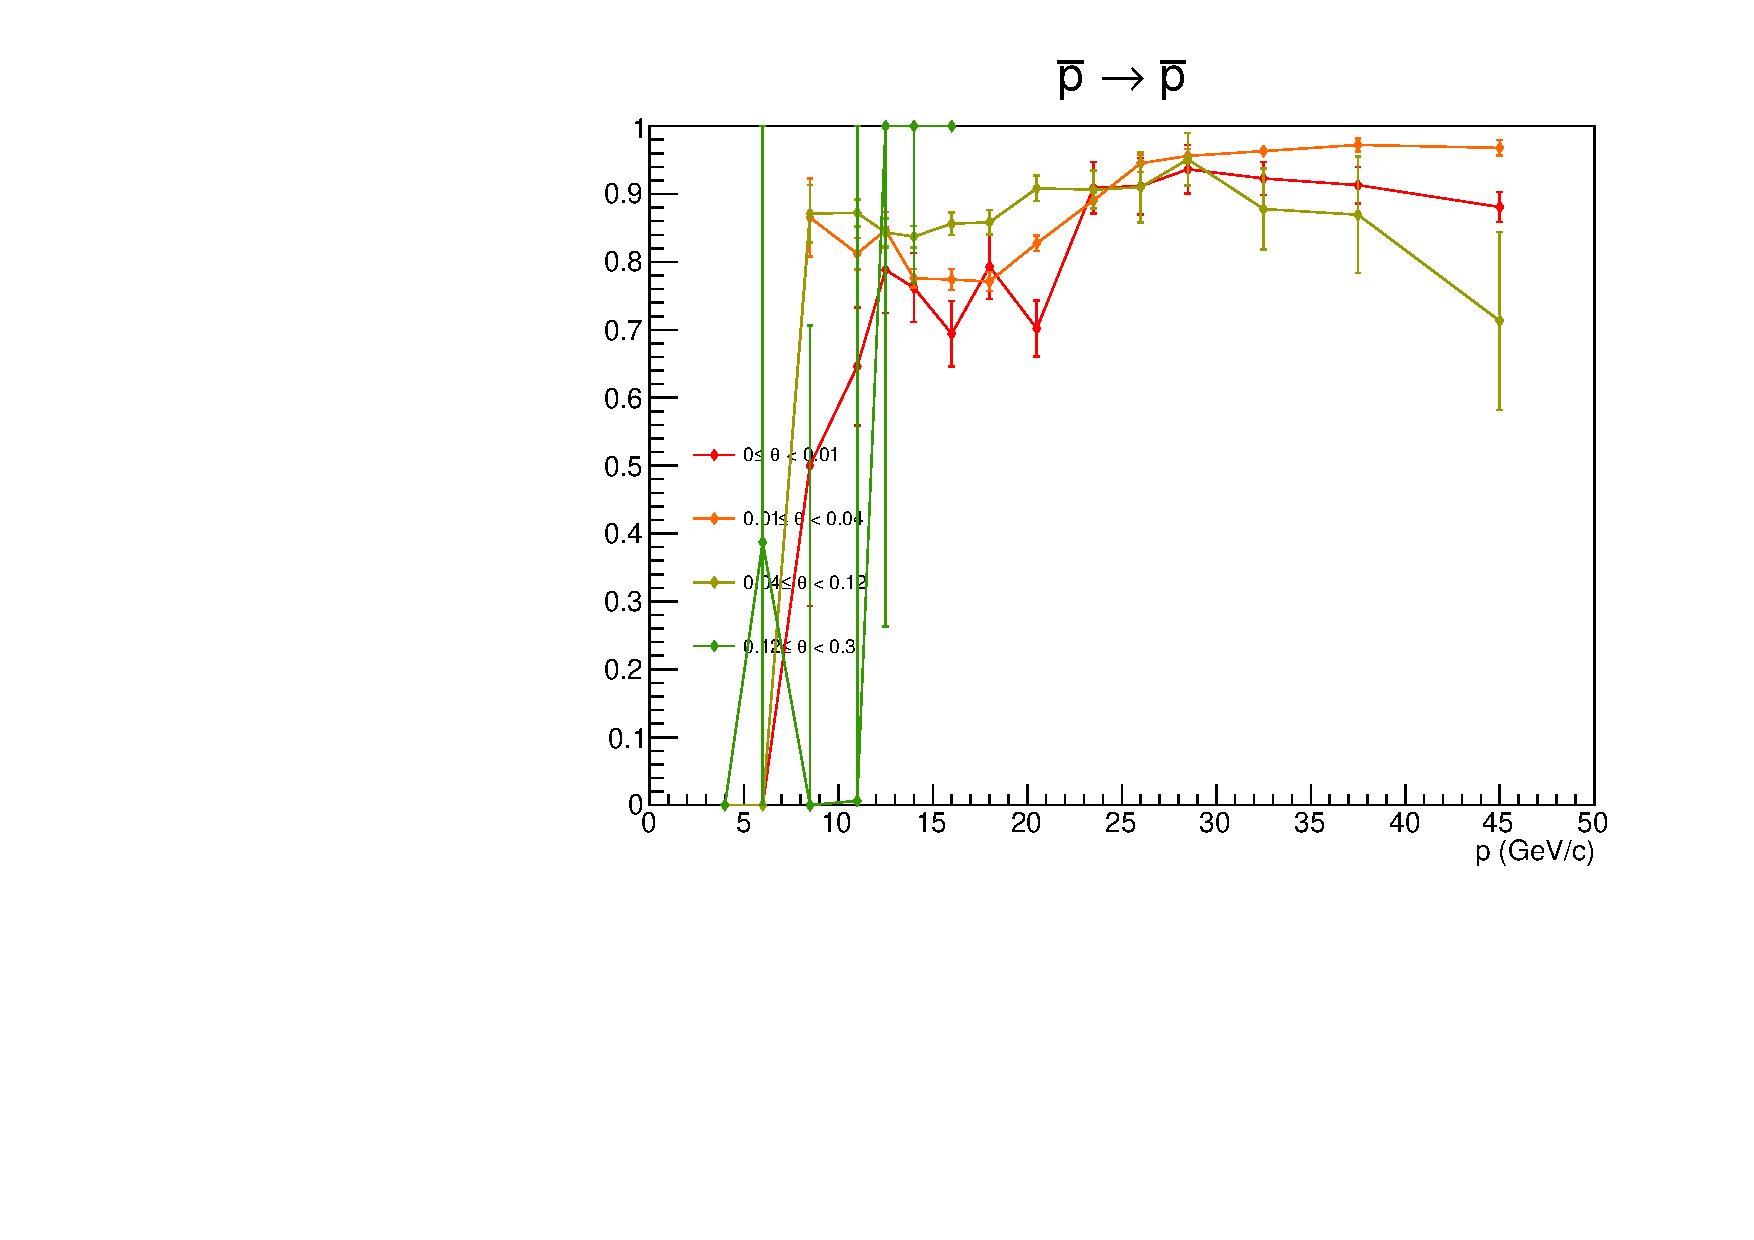
\includegraphics[scale=0.38]{./gfx/pm_p.pdf}
  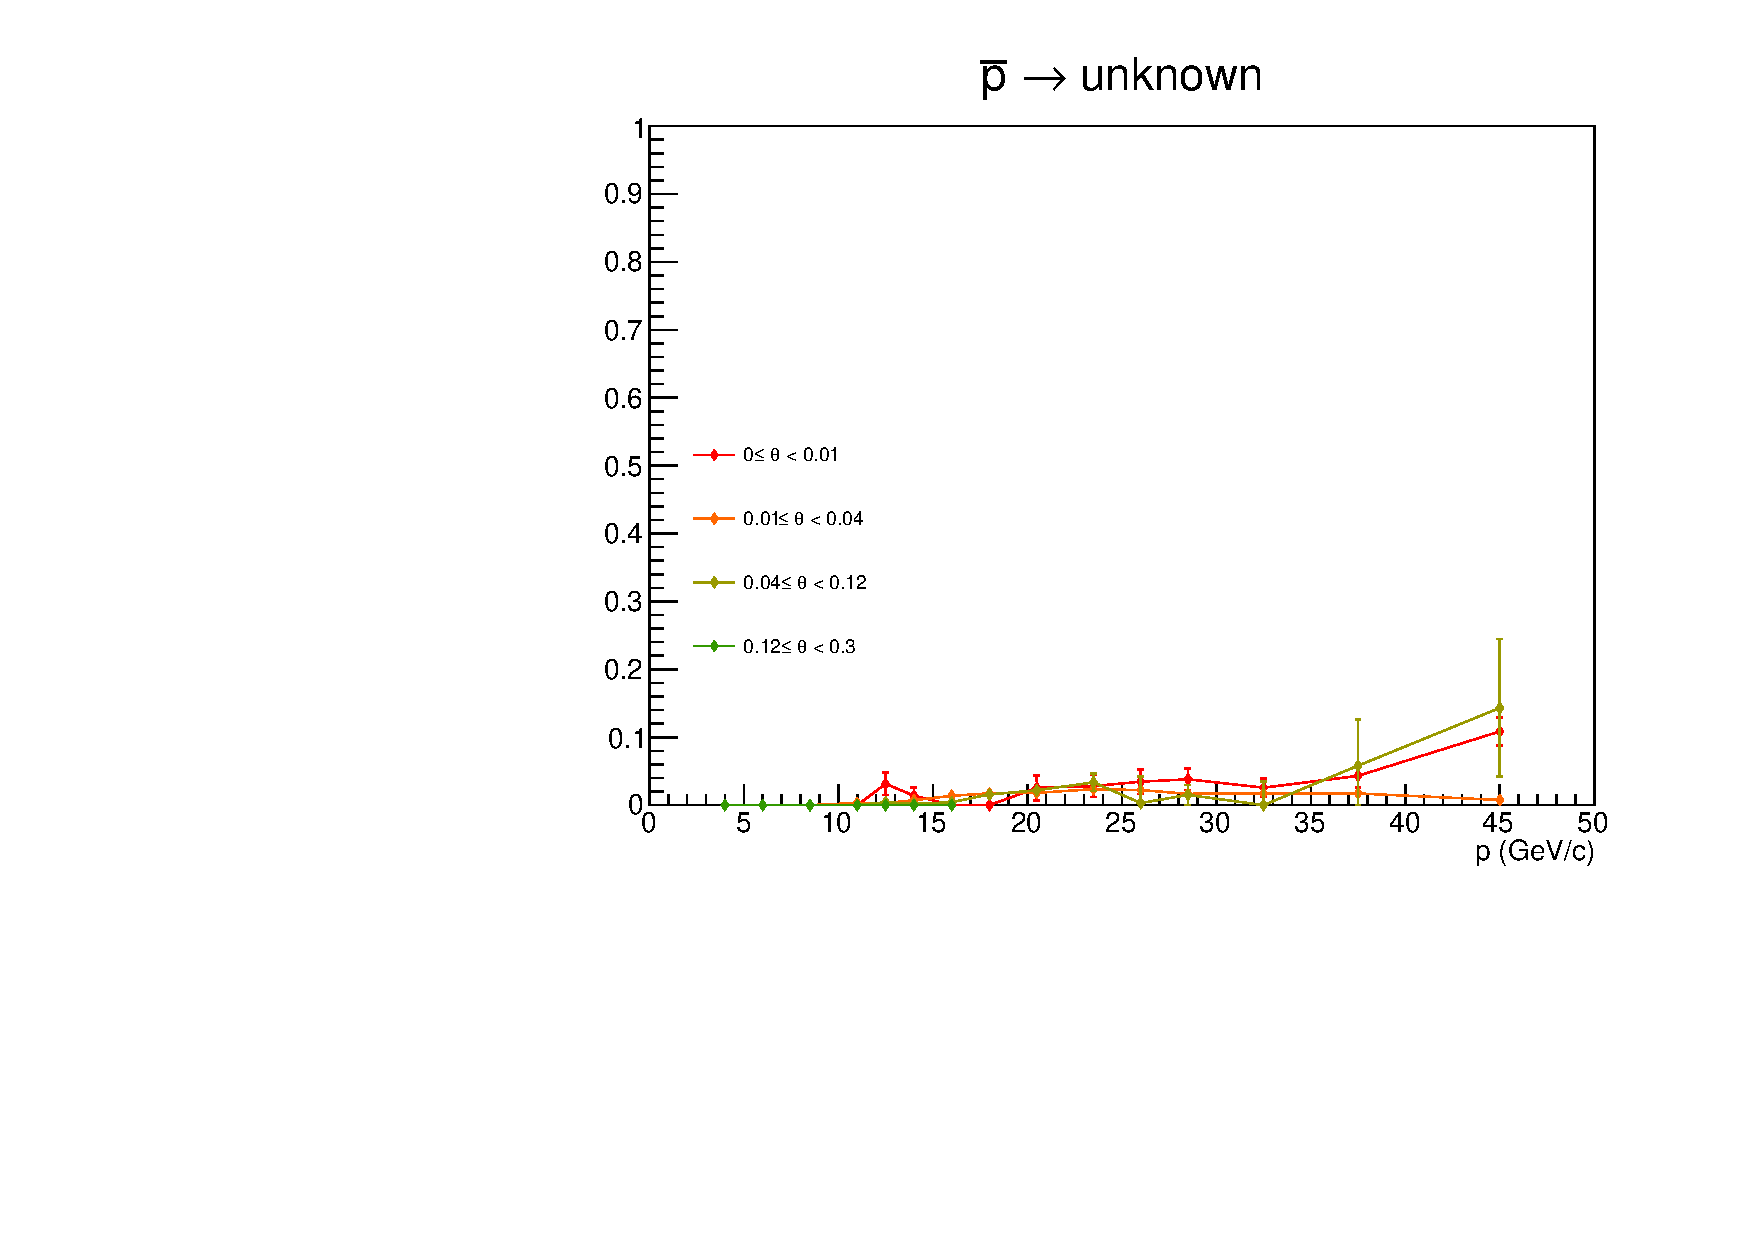
\includegraphics[scale=0.38]{./gfx/pm_u.pdf}
	\caption{Identification probabilities $\epsilon(p \rightarrow j)$ for $\bar{p}$.}
	\label{pic:Effpm}
\end{figure}


%----------------------------------------------------------------------------------------

\section{Systematic uncertainty associated to the stability of data over time}

\begin{sidewaysfigure}[p]
  \centering
	\includegraphics[scale=0.7]{./gfx/SysTimeMultpi.png}
	\caption{Same as Fig. \ref{pic:hMultTime} but for pion multiplicities.}
	\label{pic:piMultTime}
\end{sidewaysfigure}

\begin{sidewaysfigure}[p]
  \centering
	\includegraphics[scale=0.7]{./gfx/SysTimeMultk.png}
	\caption{Same as Fig. \ref{pic:hMultTime} but for kaon multiplicities.}
	\label{pic:kMultTime}
\end{sidewaysfigure}

\begin{sidewaysfigure}[p]
  \centering
	\includegraphics[scale=0.7]{./gfx/SysTimeMultp.png}
	\caption{Same as Fig. \ref{pic:hMultTime} but for proton multiplicities.}
	\label{pic:pMultTime}
\end{sidewaysfigure}

\newpage

%----------------------------------------------------------------------------------------

\section{Effect of the rescue procedure on the multiplcity sum}

\begin{figure}[!h]
  \centering
	\subfloat[]{\includegraphics[scale=0.5]{./gfx/SumVertexB4RP.png}} \\
  \subfloat[]{\includegraphics[scale=0.5]{./gfx/SumVertexBis.png}}
	\caption{Comparison of the multiplicity sum before the application  of the rescue procedure (a) and after (b) for different target slices.}
	\label{pic:Zvertexsum}
\end{figure}
 % Appendix A
%% Appendix X

\chapter{Raw multiplicity analysis}\label{app:mult}

%----------------------------------------------------------------------------------------

\section{Effect of the rescue procedure on the multiplicity sum}

An other way to look at the effect of the rescue procedure is through the multiplicity sum. Dividing the multiplicities in four bins of target, the multiplicity sum should be the same in all bins of target. Before the rescue procedure one can see that this is not the case as the multiplicity sum for the last part of the target is consistently smaller as seen in Fig.~\ref{pic:ZApp}. After the rescue procedure however, the result is as expected.

\begin{figure}[!h]
  \centering
	\subfloat[]{\includegraphics[scale=0.5]{./gfx/SumVertexB4RP.png}} \\
  \subfloat[]{\includegraphics[scale=0.5]{./gfx/SumVertexBis.png}}
	\caption{Comparison of the multiplicity sum before the application of the rescue procedure (a) and after (b) for different target slices.}
	\label{pic:ZApp}
\end{figure}

%----------------------------------------------------------------------------------------

\section{Results for raw multiplicities of identified hadrons}

The raw multiplicity results shown in this section are without any correction except the RICH unfolding correction for identified hadrons. The unidentified hadron multiplicities are displayed as a function of $z$ in bins of $x$ and staggered vertically with $y$ in Figs.~\ref{pic:rawpip} to \ref{pic:rawpm}. The charged hadron multiplicities strongly depends on $z$ as expected with a small dependence with $x$ also.

\newpage

\begin{figure}[!h]
  \includegraphics[scale=0.85]{./gfx/rawpip.pdf}
  \caption{Same as Fig.~\ref{pic:rawhp} but for positive pions.}
  \label{pic:rawpip}
\end{figure}

\begin{figure}[!h]
  \includegraphics[scale=0.85]{./gfx/rawpim.pdf}
  \caption{Same as Fig.~\ref{pic:rawhp} but for negative pions.}
  \label{pic:rawpim}
\end{figure}

\newpage

\begin{figure}[!h]
  \includegraphics[scale=0.85]{./gfx/rawkp.pdf}
  \caption{Same as Fig.~\ref{pic:rawhp} but for positive kaons.}
  \label{pic:rawkp}
\end{figure}

\begin{figure}[!h]
  \includegraphics[scale=0.85]{./gfx/rawkm.pdf}
  \caption{Same as Fig.~\ref{pic:rawhp} but for negative pions.}
  \label{pic:rawkm}
\end{figure}

\newpage

\begin{figure}[!h]
  \includegraphics[scale=0.85]{./gfx/rawpp.pdf}
  \caption{Same as Fig.~\ref{pic:rawhp} but for protons.}
  \label{pic:rawpp}
\end{figure}

\begin{figure}[!h]
  \includegraphics[scale=0.85]{./gfx/rawpm.pdf}
  \caption{Same as Fig.~\ref{pic:rawhp} but for antiprotons.}
  \label{pic:rawpm}
\end{figure}
 % Appendix B - empty template

%----------------------------------------------------------------------------------------
%	POST-CONTENT THESIS PAGES
%----------------------------------------------------------------------------------------

\cleardoublepage% Bibliography

\label{app:bibliography} % Reference the bibliography elsewhere with \autoref{app:bibliography}

\manualmark % Work-around to have small caps also here in the headline
\markboth{\spacedlowsmallcaps{\bibname}}{\spacedlowsmallcaps{\bibname}} % Work-around to have small caps also
%\phantomsection
\refstepcounter{dummy}

\addtocontents{toc}{\protect\vspace{\beforebibskip}} % Place the bibliography slightly below the rest of the document content in the table of contents
\addcontentsline{toc}{chapter}{\tocEntry{\bibname}}

\printbibliography % Bibliography

\cleardoublepage% Declaration

\refstepcounter{dummy}
\pdfbookmark[0]{Declaration}{declaration} % Bookmark name visible in a PDF viewer

\chapter*{Declaration} % Declaration section text

\thispagestyle{empty}

Put your declaration here.
\bigskip
 
\noindent\textit{\myLocation, \myTime}

\smallskip

\begin{flushright}
\begin{tabular}{m{5cm}}
\\ \hline
\centering\myName \\
\end{tabular}
\end{flushright}
 % Declaration

\cleardoublepage% Colophon (a brief description of publication or production notes relevant to the edition)

\pagestyle{empty}

\hfill

\vfill

\pdfbookmark[0]{Colophon}{colophon}

\section*{Colophon}

This document was typeset using the typographical look-and-feel \texttt{classicthesis} developed by Andr\'e Miede. The style was inspired by Robert Bringhurst's seminal book on typography ``\emph{The Elements of Typographic Style}''. \texttt{classicthesis} is available for both \LaTeX\ and \mLyX: 

\begin{center}
\url{https://bitbucket.org/amiede/classicthesis/}
\end{center}

\noindent Happy users of \texttt{classicthesis} usually send a real postcard to the author, a collection of postcards received so far is featured here: 

\begin{center}
\url{http://postcards.miede.de/}
\end{center}
 
\bigskip

\noindent\finalVersionString % Colophon

%----------------------------------------------------------------------------------------

\end{document}
